% Options for packages loaded elsewhere
\PassOptionsToPackage{unicode}{hyperref}
\PassOptionsToPackage{hyphens}{url}
%
\documentclass[
]{article}
\usepackage{lmodern}
\usepackage{amssymb,amsmath}
\usepackage{ifxetex,ifluatex}
\ifnum 0\ifxetex 1\fi\ifluatex 1\fi=0 % if pdftex
  \usepackage[T1]{fontenc}
  \usepackage[utf8]{inputenc}
  \usepackage{textcomp} % provide euro and other symbols
\else % if luatex or xetex
  \usepackage{unicode-math}
  \defaultfontfeatures{Scale=MatchLowercase}
  \defaultfontfeatures[\rmfamily]{Ligatures=TeX,Scale=1}
\fi
% Use upquote if available, for straight quotes in verbatim environments
\IfFileExists{upquote.sty}{\usepackage{upquote}}{}
\IfFileExists{microtype.sty}{% use microtype if available
  \usepackage[]{microtype}
  \UseMicrotypeSet[protrusion]{basicmath} % disable protrusion for tt fonts
}{}
\makeatletter
\@ifundefined{KOMAClassName}{% if non-KOMA class
  \IfFileExists{parskip.sty}{%
    \usepackage{parskip}
  }{% else
    \setlength{\parindent}{0pt}
    \setlength{\parskip}{6pt plus 2pt minus 1pt}}
}{% if KOMA class
  \KOMAoptions{parskip=half}}
\makeatother
\usepackage{xcolor}
\IfFileExists{xurl.sty}{\usepackage{xurl}}{} % add URL line breaks if available
\IfFileExists{bookmark.sty}{\usepackage{bookmark}}{\usepackage{hyperref}}
\hypersetup{
  pdftitle={Analysis 1: Main Analysis with Original and Mail-In Data},
  pdfauthor={Fan Lu \& Gento Kato},
  hidelinks,
  pdfcreator={LaTeX via pandoc}}
\urlstyle{same} % disable monospaced font for URLs
\usepackage[margin=1in]{geometry}
\usepackage{color}
\usepackage{fancyvrb}
\newcommand{\VerbBar}{|}
\newcommand{\VERB}{\Verb[commandchars=\\\{\}]}
\DefineVerbatimEnvironment{Highlighting}{Verbatim}{commandchars=\\\{\}}
% Add ',fontsize=\small' for more characters per line
\usepackage{framed}
\definecolor{shadecolor}{RGB}{248,248,248}
\newenvironment{Shaded}{\begin{snugshade}}{\end{snugshade}}
\newcommand{\AlertTok}[1]{\textcolor[rgb]{0.94,0.16,0.16}{#1}}
\newcommand{\AnnotationTok}[1]{\textcolor[rgb]{0.56,0.35,0.01}{\textbf{\textit{#1}}}}
\newcommand{\AttributeTok}[1]{\textcolor[rgb]{0.77,0.63,0.00}{#1}}
\newcommand{\BaseNTok}[1]{\textcolor[rgb]{0.00,0.00,0.81}{#1}}
\newcommand{\BuiltInTok}[1]{#1}
\newcommand{\CharTok}[1]{\textcolor[rgb]{0.31,0.60,0.02}{#1}}
\newcommand{\CommentTok}[1]{\textcolor[rgb]{0.56,0.35,0.01}{\textit{#1}}}
\newcommand{\CommentVarTok}[1]{\textcolor[rgb]{0.56,0.35,0.01}{\textbf{\textit{#1}}}}
\newcommand{\ConstantTok}[1]{\textcolor[rgb]{0.00,0.00,0.00}{#1}}
\newcommand{\ControlFlowTok}[1]{\textcolor[rgb]{0.13,0.29,0.53}{\textbf{#1}}}
\newcommand{\DataTypeTok}[1]{\textcolor[rgb]{0.13,0.29,0.53}{#1}}
\newcommand{\DecValTok}[1]{\textcolor[rgb]{0.00,0.00,0.81}{#1}}
\newcommand{\DocumentationTok}[1]{\textcolor[rgb]{0.56,0.35,0.01}{\textbf{\textit{#1}}}}
\newcommand{\ErrorTok}[1]{\textcolor[rgb]{0.64,0.00,0.00}{\textbf{#1}}}
\newcommand{\ExtensionTok}[1]{#1}
\newcommand{\FloatTok}[1]{\textcolor[rgb]{0.00,0.00,0.81}{#1}}
\newcommand{\FunctionTok}[1]{\textcolor[rgb]{0.00,0.00,0.00}{#1}}
\newcommand{\ImportTok}[1]{#1}
\newcommand{\InformationTok}[1]{\textcolor[rgb]{0.56,0.35,0.01}{\textbf{\textit{#1}}}}
\newcommand{\KeywordTok}[1]{\textcolor[rgb]{0.13,0.29,0.53}{\textbf{#1}}}
\newcommand{\NormalTok}[1]{#1}
\newcommand{\OperatorTok}[1]{\textcolor[rgb]{0.81,0.36,0.00}{\textbf{#1}}}
\newcommand{\OtherTok}[1]{\textcolor[rgb]{0.56,0.35,0.01}{#1}}
\newcommand{\PreprocessorTok}[1]{\textcolor[rgb]{0.56,0.35,0.01}{\textit{#1}}}
\newcommand{\RegionMarkerTok}[1]{#1}
\newcommand{\SpecialCharTok}[1]{\textcolor[rgb]{0.00,0.00,0.00}{#1}}
\newcommand{\SpecialStringTok}[1]{\textcolor[rgb]{0.31,0.60,0.02}{#1}}
\newcommand{\StringTok}[1]{\textcolor[rgb]{0.31,0.60,0.02}{#1}}
\newcommand{\VariableTok}[1]{\textcolor[rgb]{0.00,0.00,0.00}{#1}}
\newcommand{\VerbatimStringTok}[1]{\textcolor[rgb]{0.31,0.60,0.02}{#1}}
\newcommand{\WarningTok}[1]{\textcolor[rgb]{0.56,0.35,0.01}{\textbf{\textit{#1}}}}
\usepackage{graphicx,grffile}
\makeatletter
\def\maxwidth{\ifdim\Gin@nat@width>\linewidth\linewidth\else\Gin@nat@width\fi}
\def\maxheight{\ifdim\Gin@nat@height>\textheight\textheight\else\Gin@nat@height\fi}
\makeatother
% Scale images if necessary, so that they will not overflow the page
% margins by default, and it is still possible to overwrite the defaults
% using explicit options in \includegraphics[width, height, ...]{}
\setkeys{Gin}{width=\maxwidth,height=\maxheight,keepaspectratio}
% Set default figure placement to htbp
\makeatletter
\def\fps@figure{htbp}
\makeatother
\setlength{\emergencystretch}{3em} % prevent overfull lines
\providecommand{\tightlist}{%
  \setlength{\itemsep}{0pt}\setlength{\parskip}{0pt}}
\setcounter{secnumdepth}{-\maxdimen} % remove section numbering
\usepackage{bookmark}
\usepackage{xltxtra}
\usepackage{zxjatype}
\usepackage[ipa]{zxjafont}

\title{Analysis 1: Main Analysis with Original and Mail-In Data}
\author{Fan Lu \& Gento Kato}
\date{January 26, 2021}

\begin{document}
\maketitle

\hypertarget{analytical-strategy}{%
\section{Analytical Strategy}\label{analytical-strategy}}

\hypertarget{variables}{%
\subsection{Variables}\label{variables}}

\begin{itemize}
\item
  Outcome: Foreigner Suffrage (min 0, max 1)
\item
  Mediator 1: (Objective) Political Knowledge (min = 0, max = 1)
\item
  Mediator 2: Ideology (min 0 = left/liberal, max 1 =
  right/conservative)
\item
  Mediator 3: LDP - DPJ FT (min 0 = favor DPJ, max 1 = favor LDP)
\item
  Mediator 4: Favorability of South Korea (min = 0, max = 1)\\
\item
  Mediator 5: Favorability of China (min = 0, max = 1)\\
\item
  Mediator 6: Favorability of USA (min = 0, max = 1)\\
\item
  Mediator 7: Income (percentile, min = 0, max = 1)
\item
  Independent Variable: University Education (0 = Junior College or
  Less, 1 = University or More)
\item
  Moderator 1: Gender (0 = Female, 1 = Male), This means that all
  ``base'' coefficients are for female.
\item
  Moderator 2: Age (by 10 years, centered at 20). Reasoning: Two trends
  may influence the role of university education. (1) There is an
  evident increase in number of university graduates over the years,
  especially among women. This trend may impies that university
  experience may be more gendered in the past than today. (2) There is a
  trend of ``internationalization'' in university education in recent
  days. Therefore, the diversifying and liberalizing effect of education
  may be stronger for younger generation.
\item
  Control 1: Percent in life residing locally. More locally-identified
  individuals may dislike outsiders more.
\item
  Control 2: (ZIP level) Residing in densely inhabited district (DID)
\item
  Control 3: (ZIP level) Percent of foreigners in neighborhood
  (transformed by square root)\\
\item
  Control 4: (ZIP level) Percent of university graduates in neighborhood
  (by 10 percent)
\item
  Control 5: (Municipality level) Percent of residents residing in DID
\item
  Control 6: (Municipality level) Percent of foreigners (transformed by
  square root)
\item
  Control 7: (Municipality level) Percent of university graduates (by 10
  percent)
\end{itemize}

\hypertarget{subset-data}{%
\subsection{Subset Data}\label{subset-data}}

Analysis is conducted on the following subset.

If age - years of local ZIP residence is 15 or smaller. 15 is the age of
entering high school in Japan. Assuming that an individual is living in
the local ZIP continuously, this condition implies that one spend
significant time before college in the ZIP of current residence. This
filters out the possibility that education changes attitudes through the
movement in residence.

\hypertarget{modeling-strategy}{%
\subsection{Modeling Strategy}\label{modeling-strategy}}

All models are estimated by OLS. For outcome model, alternative model is
estimated by the multinomial logit model, with 3 category DV (disagree,
neither, agree), with disagree as a reference category.

\hypertarget{robustness-check-in-this-file}{%
\subsection{Robustness Check (in this
file)}\label{robustness-check-in-this-file}}

SIFCCT has one special survey where they conducted a survey through
mail. Mail survey contains identical set of variables as online survey.
So I replicated the analysis with the mail survey.

\hypertarget{preparation}{%
\section{Preparation}\label{preparation}}

\begin{Shaded}
\begin{Highlighting}[]
\CommentTok{## Clean Up Space}
\KeywordTok{rm}\NormalTok{(}\DataTypeTok{list=}\KeywordTok{ls}\NormalTok{())}

\CommentTok{## Set Working Directory (Automatically) ##}
\KeywordTok{require}\NormalTok{(rstudioapi); }\KeywordTok{require}\NormalTok{(rprojroot)}
\ControlFlowTok{if}\NormalTok{ (rstudioapi}\OperatorTok{::}\KeywordTok{isAvailable}\NormalTok{()}\OperatorTok{==}\OtherTok{TRUE}\NormalTok{) \{}
  \KeywordTok{setwd}\NormalTok{(}\KeywordTok{dirname}\NormalTok{(rstudioapi}\OperatorTok{::}\KeywordTok{getActiveDocumentContext}\NormalTok{()}\OperatorTok{$}\NormalTok{path)); }
\NormalTok{\} }
\NormalTok{projdir <-}\StringTok{ }\KeywordTok{find_root}\NormalTok{(}\KeywordTok{has_file}\NormalTok{(}\StringTok{"thisishome.txt"}\NormalTok{))}
\KeywordTok{cat}\NormalTok{(}\KeywordTok{paste}\NormalTok{(}\StringTok{"Working Directory Set to:}\CharTok{\textbackslash{}n}\StringTok{"}\NormalTok{,projdir))}
\end{Highlighting}
\end{Shaded}

\begin{verbatim}
## Working Directory Set to:
##  /home/gentok/GoogleDrive/Projects/Fan-Gento-Lab/ForeignerJapan
\end{verbatim}

\begin{Shaded}
\begin{Highlighting}[]
\KeywordTok{setwd}\NormalTok{(projdir)}

\CommentTok{## Original Data}
\NormalTok{datadir1a <-}\StringTok{ }\KeywordTok{paste0}\NormalTok{(projdir, }\StringTok{"/data/sifcct_zip_latest_v5.rds"}\NormalTok{)}
\NormalTok{datadir1b <-}\StringTok{ }\KeywordTok{paste0}\NormalTok{(projdir, }\StringTok{"/data/sifcct_zip_latest_panel_v5.rds"}\NormalTok{)}
\NormalTok{datadir2 <-}\StringTok{ }\KeywordTok{paste0}\NormalTok{(projdir, }\StringTok{"/data/mail_zip_latest_v5.rds"}\NormalTok{)}

\CommentTok{## packages}
\KeywordTok{require}\NormalTok{(sandwich)}
\KeywordTok{require}\NormalTok{(lmtest)}
\KeywordTok{require}\NormalTok{(MASS)}
\CommentTok{# devtools::install_github("tidyverse/ggplot2") # Need development version (as of Dec 31, 2019)}
\KeywordTok{require}\NormalTok{(ggplot2)}
\KeywordTok{require}\NormalTok{(texreg)}
\KeywordTok{require}\NormalTok{(mlogit)}
\KeywordTok{require}\NormalTok{(Formula)}
\end{Highlighting}
\end{Shaded}

\hypertarget{import-and-clean-data}{%
\section{Import and clean data}\label{import-and-clean-data}}

\begin{Shaded}
\begin{Highlighting}[]
\CommentTok{###################}
\CommentTok{## SIFCCT Online ##}
\CommentTok{###################}

\NormalTok{sifcct <-}\StringTok{ }\KeywordTok{rbind}\NormalTok{(}\KeywordTok{readRDS}\NormalTok{(datadir1a),}\KeywordTok{readRDS}\NormalTok{(datadir1b))}

\CommentTok{## Knowledge Variable (Replaced)}
\NormalTok{sifcct}\OperatorTok{$}\NormalTok{knowledge[sifcct}\OperatorTok{$}\NormalTok{panel}\OperatorTok{==}\DecValTok{1} \OperatorTok{&}\StringTok{ }\NormalTok{sifcct}\OperatorTok{$}\NormalTok{wave}\OperatorTok{==}\DecValTok{2}\NormalTok{] <-}\StringTok{ }\NormalTok{sifcct}\OperatorTok{$}\NormalTok{knowledge[sifcct}\OperatorTok{$}\NormalTok{panel}\OperatorTok{==}\DecValTok{1} \OperatorTok{&}\StringTok{ }\NormalTok{sifcct}\OperatorTok{$}\NormalTok{wave}\OperatorTok{==}\DecValTok{1}\NormalTok{][}\KeywordTok{match}\NormalTok{(sifcct}\OperatorTok{$}\NormalTok{panelid[sifcct}\OperatorTok{$}\NormalTok{panel}\OperatorTok{==}\DecValTok{1} \OperatorTok{&}\StringTok{ }\NormalTok{sifcct}\OperatorTok{$}\NormalTok{wave}\OperatorTok{==}\DecValTok{2}\NormalTok{],sifcct}\OperatorTok{$}\NormalTok{panelid[sifcct}\OperatorTok{$}\NormalTok{panel}\OperatorTok{==}\DecValTok{1} \OperatorTok{&}\StringTok{ }\NormalTok{sifcct}\OperatorTok{$}\NormalTok{wave}\OperatorTok{==}\DecValTok{1}\NormalTok{])]}
\NormalTok{sifcct}\OperatorTok{$}\NormalTok{knowledge[sifcct}\OperatorTok{$}\NormalTok{panel}\OperatorTok{==}\DecValTok{1} \OperatorTok{&}\StringTok{ }\NormalTok{sifcct}\OperatorTok{$}\NormalTok{wave}\OperatorTok{==}\DecValTok{3}\NormalTok{] <-}\StringTok{ }\NormalTok{sifcct}\OperatorTok{$}\NormalTok{knowledge[sifcct}\OperatorTok{$}\NormalTok{panel}\OperatorTok{==}\DecValTok{1} \OperatorTok{&}\StringTok{ }\NormalTok{sifcct}\OperatorTok{$}\NormalTok{wave}\OperatorTok{==}\DecValTok{1}\NormalTok{][}\KeywordTok{match}\NormalTok{(sifcct}\OperatorTok{$}\NormalTok{panelid[sifcct}\OperatorTok{$}\NormalTok{panel}\OperatorTok{==}\DecValTok{1} \OperatorTok{&}\StringTok{ }\NormalTok{sifcct}\OperatorTok{$}\NormalTok{wave}\OperatorTok{==}\DecValTok{3}\NormalTok{],sifcct}\OperatorTok{$}\NormalTok{panelid[sifcct}\OperatorTok{$}\NormalTok{panel}\OperatorTok{==}\DecValTok{1} \OperatorTok{&}\StringTok{ }\NormalTok{sifcct}\OperatorTok{$}\NormalTok{wave}\OperatorTok{==}\DecValTok{1}\NormalTok{])]}
\NormalTok{sifcct}\OperatorTok{$}\NormalTok{knowledge[sifcct}\OperatorTok{$}\NormalTok{panel}\OperatorTok{==}\DecValTok{1} \OperatorTok{&}\StringTok{ }\NormalTok{sifcct}\OperatorTok{$}\NormalTok{wave}\OperatorTok{==}\DecValTok{4}\NormalTok{] <-}\StringTok{ }\NormalTok{sifcct}\OperatorTok{$}\NormalTok{knowledge[sifcct}\OperatorTok{$}\NormalTok{panel}\OperatorTok{==}\DecValTok{1} \OperatorTok{&}\StringTok{ }\NormalTok{sifcct}\OperatorTok{$}\NormalTok{wave}\OperatorTok{==}\DecValTok{1}\NormalTok{][}\KeywordTok{match}\NormalTok{(sifcct}\OperatorTok{$}\NormalTok{panelid[sifcct}\OperatorTok{$}\NormalTok{panel}\OperatorTok{==}\DecValTok{1} \OperatorTok{&}\StringTok{ }\NormalTok{sifcct}\OperatorTok{$}\NormalTok{wave}\OperatorTok{==}\DecValTok{4}\NormalTok{],sifcct}\OperatorTok{$}\NormalTok{panelid[sifcct}\OperatorTok{$}\NormalTok{panel}\OperatorTok{==}\DecValTok{1} \OperatorTok{&}\StringTok{ }\NormalTok{sifcct}\OperatorTok{$}\NormalTok{wave}\OperatorTok{==}\DecValTok{1}\NormalTok{])]}
\NormalTok{sifcct}\OperatorTok{$}\NormalTok{knowledge[sifcct}\OperatorTok{$}\NormalTok{panel}\OperatorTok{==}\DecValTok{1} \OperatorTok{&}\StringTok{ }\NormalTok{sifcct}\OperatorTok{$}\NormalTok{wave}\OperatorTok{==}\DecValTok{5}\NormalTok{] <-}\StringTok{ }\NormalTok{sifcct}\OperatorTok{$}\NormalTok{knowledge[sifcct}\OperatorTok{$}\NormalTok{panel}\OperatorTok{==}\DecValTok{1} \OperatorTok{&}\StringTok{ }\NormalTok{sifcct}\OperatorTok{$}\NormalTok{wave}\OperatorTok{==}\DecValTok{1}\NormalTok{][}\KeywordTok{match}\NormalTok{(sifcct}\OperatorTok{$}\NormalTok{panelid[sifcct}\OperatorTok{$}\NormalTok{panel}\OperatorTok{==}\DecValTok{1} \OperatorTok{&}\StringTok{ }\NormalTok{sifcct}\OperatorTok{$}\NormalTok{wave}\OperatorTok{==}\DecValTok{5}\NormalTok{],sifcct}\OperatorTok{$}\NormalTok{panelid[sifcct}\OperatorTok{$}\NormalTok{panel}\OperatorTok{==}\DecValTok{1} \OperatorTok{&}\StringTok{ }\NormalTok{sifcct}\OperatorTok{$}\NormalTok{wave}\OperatorTok{==}\DecValTok{1}\NormalTok{])]}
\NormalTok{sifcct}\OperatorTok{$}\NormalTok{knowledge[sifcct}\OperatorTok{$}\NormalTok{panel}\OperatorTok{==}\DecValTok{1} \OperatorTok{&}\StringTok{ }\NormalTok{sifcct}\OperatorTok{$}\NormalTok{wave}\OperatorTok{==}\DecValTok{6}\NormalTok{] <-}\StringTok{ }\NormalTok{sifcct}\OperatorTok{$}\NormalTok{knowledge[sifcct}\OperatorTok{$}\NormalTok{panel}\OperatorTok{==}\DecValTok{1} \OperatorTok{&}\StringTok{ }\NormalTok{sifcct}\OperatorTok{$}\NormalTok{wave}\OperatorTok{==}\DecValTok{1}\NormalTok{][}\KeywordTok{match}\NormalTok{(sifcct}\OperatorTok{$}\NormalTok{panelid[sifcct}\OperatorTok{$}\NormalTok{panel}\OperatorTok{==}\DecValTok{1} \OperatorTok{&}\StringTok{ }\NormalTok{sifcct}\OperatorTok{$}\NormalTok{wave}\OperatorTok{==}\DecValTok{6}\NormalTok{],sifcct}\OperatorTok{$}\NormalTok{panelid[sifcct}\OperatorTok{$}\NormalTok{panel}\OperatorTok{==}\DecValTok{1} \OperatorTok{&}\StringTok{ }\NormalTok{sifcct}\OperatorTok{$}\NormalTok{wave}\OperatorTok{==}\DecValTok{1}\NormalTok{])]}
\NormalTok{sifcct}\OperatorTok{$}\NormalTok{knowledge[sifcct}\OperatorTok{$}\NormalTok{panel}\OperatorTok{==}\DecValTok{1} \OperatorTok{&}\StringTok{ }\NormalTok{sifcct}\OperatorTok{$}\NormalTok{wave}\OperatorTok{==}\DecValTok{7}\NormalTok{] <-}\StringTok{ }\NormalTok{sifcct}\OperatorTok{$}\NormalTok{knowledge[sifcct}\OperatorTok{$}\NormalTok{panel}\OperatorTok{==}\DecValTok{1} \OperatorTok{&}\StringTok{ }\NormalTok{sifcct}\OperatorTok{$}\NormalTok{wave}\OperatorTok{==}\DecValTok{1}\NormalTok{][}\KeywordTok{match}\NormalTok{(sifcct}\OperatorTok{$}\NormalTok{panelid[sifcct}\OperatorTok{$}\NormalTok{panel}\OperatorTok{==}\DecValTok{1} \OperatorTok{&}\StringTok{ }\NormalTok{sifcct}\OperatorTok{$}\NormalTok{wave}\OperatorTok{==}\DecValTok{7}\NormalTok{],sifcct}\OperatorTok{$}\NormalTok{panelid[sifcct}\OperatorTok{$}\NormalTok{panel}\OperatorTok{==}\DecValTok{1} \OperatorTok{&}\StringTok{ }\NormalTok{sifcct}\OperatorTok{$}\NormalTok{wave}\OperatorTok{==}\DecValTok{1}\NormalTok{])]}
\NormalTok{sifcct}\OperatorTok{$}\NormalTok{knowledge[sifcct}\OperatorTok{$}\NormalTok{panel}\OperatorTok{==}\DecValTok{1} \OperatorTok{&}\StringTok{ }\NormalTok{sifcct}\OperatorTok{$}\NormalTok{wave}\OperatorTok{==}\DecValTok{8}\NormalTok{] <-}\StringTok{ }\NormalTok{sifcct}\OperatorTok{$}\NormalTok{knowledge[sifcct}\OperatorTok{$}\NormalTok{panel}\OperatorTok{==}\DecValTok{1} \OperatorTok{&}\StringTok{ }\NormalTok{sifcct}\OperatorTok{$}\NormalTok{wave}\OperatorTok{==}\DecValTok{1}\NormalTok{][}\KeywordTok{match}\NormalTok{(sifcct}\OperatorTok{$}\NormalTok{panelid[sifcct}\OperatorTok{$}\NormalTok{panel}\OperatorTok{==}\DecValTok{1} \OperatorTok{&}\StringTok{ }\NormalTok{sifcct}\OperatorTok{$}\NormalTok{wave}\OperatorTok{==}\DecValTok{8}\NormalTok{],sifcct}\OperatorTok{$}\NormalTok{panelid[sifcct}\OperatorTok{$}\NormalTok{panel}\OperatorTok{==}\DecValTok{1} \OperatorTok{&}\StringTok{ }\NormalTok{sifcct}\OperatorTok{$}\NormalTok{wave}\OperatorTok{==}\DecValTok{1}\NormalTok{])]}
\NormalTok{sifcct}\OperatorTok{$}\NormalTok{knowledge[sifcct}\OperatorTok{$}\NormalTok{panel}\OperatorTok{==}\DecValTok{1} \OperatorTok{&}\StringTok{ }\NormalTok{sifcct}\OperatorTok{$}\NormalTok{wave}\OperatorTok{==}\DecValTok{9}\NormalTok{] <-}\StringTok{ }\NormalTok{sifcct}\OperatorTok{$}\NormalTok{knowledge[sifcct}\OperatorTok{$}\NormalTok{panel}\OperatorTok{==}\DecValTok{1} \OperatorTok{&}\StringTok{ }\NormalTok{sifcct}\OperatorTok{$}\NormalTok{wave}\OperatorTok{==}\DecValTok{1}\NormalTok{][}\KeywordTok{match}\NormalTok{(sifcct}\OperatorTok{$}\NormalTok{panelid[sifcct}\OperatorTok{$}\NormalTok{panel}\OperatorTok{==}\DecValTok{1} \OperatorTok{&}\StringTok{ }\NormalTok{sifcct}\OperatorTok{$}\NormalTok{wave}\OperatorTok{==}\DecValTok{9}\NormalTok{],sifcct}\OperatorTok{$}\NormalTok{panelid[sifcct}\OperatorTok{$}\NormalTok{panel}\OperatorTok{==}\DecValTok{1} \OperatorTok{&}\StringTok{ }\NormalTok{sifcct}\OperatorTok{$}\NormalTok{wave}\OperatorTok{==}\DecValTok{1}\NormalTok{])]}
\NormalTok{sifcct}\OperatorTok{$}\NormalTok{knowledge[sifcct}\OperatorTok{$}\NormalTok{panel}\OperatorTok{==}\DecValTok{1} \OperatorTok{&}\StringTok{ }\NormalTok{sifcct}\OperatorTok{$}\NormalTok{wave}\OperatorTok{==}\DecValTok{10}\NormalTok{] <-}\StringTok{ }\NormalTok{sifcct}\OperatorTok{$}\NormalTok{knowledge[sifcct}\OperatorTok{$}\NormalTok{panel}\OperatorTok{==}\DecValTok{1} \OperatorTok{&}\StringTok{ }\NormalTok{sifcct}\OperatorTok{$}\NormalTok{wave}\OperatorTok{==}\DecValTok{1}\NormalTok{][}\KeywordTok{match}\NormalTok{(sifcct}\OperatorTok{$}\NormalTok{panelid[sifcct}\OperatorTok{$}\NormalTok{panel}\OperatorTok{==}\DecValTok{1} \OperatorTok{&}\StringTok{ }\NormalTok{sifcct}\OperatorTok{$}\NormalTok{wave}\OperatorTok{==}\DecValTok{10}\NormalTok{],sifcct}\OperatorTok{$}\NormalTok{panelid[sifcct}\OperatorTok{$}\NormalTok{panel}\OperatorTok{==}\DecValTok{1} \OperatorTok{&}\StringTok{ }\NormalTok{sifcct}\OperatorTok{$}\NormalTok{wave}\OperatorTok{==}\DecValTok{1}\NormalTok{])]}
\NormalTok{sifcct}\OperatorTok{$}\NormalTok{knowledge[sifcct}\OperatorTok{$}\NormalTok{panel}\OperatorTok{==}\DecValTok{1} \OperatorTok{&}\StringTok{ }\NormalTok{sifcct}\OperatorTok{$}\NormalTok{wave}\OperatorTok{==}\DecValTok{11}\NormalTok{] <-}\StringTok{ }\NormalTok{sifcct}\OperatorTok{$}\NormalTok{knowledge[sifcct}\OperatorTok{$}\NormalTok{panel}\OperatorTok{==}\DecValTok{1} \OperatorTok{&}\StringTok{ }\NormalTok{sifcct}\OperatorTok{$}\NormalTok{wave}\OperatorTok{==}\DecValTok{1}\NormalTok{][}\KeywordTok{match}\NormalTok{(sifcct}\OperatorTok{$}\NormalTok{panelid[sifcct}\OperatorTok{$}\NormalTok{panel}\OperatorTok{==}\DecValTok{1} \OperatorTok{&}\StringTok{ }\NormalTok{sifcct}\OperatorTok{$}\NormalTok{wave}\OperatorTok{==}\DecValTok{11}\NormalTok{],sifcct}\OperatorTok{$}\NormalTok{panelid[sifcct}\OperatorTok{$}\NormalTok{panel}\OperatorTok{==}\DecValTok{1} \OperatorTok{&}\StringTok{ }\NormalTok{sifcct}\OperatorTok{$}\NormalTok{wave}\OperatorTok{==}\DecValTok{1}\NormalTok{])]}
\NormalTok{sifcct}\OperatorTok{$}\NormalTok{knowledge[sifcct}\OperatorTok{$}\NormalTok{panel}\OperatorTok{==}\DecValTok{1} \OperatorTok{&}\StringTok{ }\NormalTok{sifcct}\OperatorTok{$}\NormalTok{wave}\OperatorTok{==}\DecValTok{12}\NormalTok{] <-}\StringTok{ }\NormalTok{sifcct}\OperatorTok{$}\NormalTok{knowledge[sifcct}\OperatorTok{$}\NormalTok{panel}\OperatorTok{==}\DecValTok{1} \OperatorTok{&}\StringTok{ }\NormalTok{sifcct}\OperatorTok{$}\NormalTok{wave}\OperatorTok{==}\DecValTok{1}\NormalTok{][}\KeywordTok{match}\NormalTok{(sifcct}\OperatorTok{$}\NormalTok{panelid[sifcct}\OperatorTok{$}\NormalTok{panel}\OperatorTok{==}\DecValTok{1} \OperatorTok{&}\StringTok{ }\NormalTok{sifcct}\OperatorTok{$}\NormalTok{wave}\OperatorTok{==}\DecValTok{12}\NormalTok{],sifcct}\OperatorTok{$}\NormalTok{panelid[sifcct}\OperatorTok{$}\NormalTok{panel}\OperatorTok{==}\DecValTok{1} \OperatorTok{&}\StringTok{ }\NormalTok{sifcct}\OperatorTok{$}\NormalTok{wave}\OperatorTok{==}\DecValTok{1}\NormalTok{])]}
\CommentTok{## Knowledge Variable (Replaced)}
\NormalTok{sifcct}\OperatorTok{$}\NormalTok{knowledge[sifcct}\OperatorTok{$}\NormalTok{panel}\OperatorTok{==}\DecValTok{1} \OperatorTok{&}\StringTok{ }\NormalTok{sifcct}\OperatorTok{$}\NormalTok{wave}\OperatorTok{==}\DecValTok{14}\NormalTok{] <-}\StringTok{ }\NormalTok{sifcct}\OperatorTok{$}\NormalTok{knowledge[sifcct}\OperatorTok{$}\NormalTok{panel}\OperatorTok{==}\DecValTok{1} \OperatorTok{&}\StringTok{ }\NormalTok{sifcct}\OperatorTok{$}\NormalTok{wave}\OperatorTok{==}\DecValTok{13}\NormalTok{][}\KeywordTok{match}\NormalTok{(sifcct}\OperatorTok{$}\NormalTok{panelid[sifcct}\OperatorTok{$}\NormalTok{panel}\OperatorTok{==}\DecValTok{1} \OperatorTok{&}\StringTok{ }\NormalTok{sifcct}\OperatorTok{$}\NormalTok{wave}\OperatorTok{==}\DecValTok{14}\NormalTok{],sifcct}\OperatorTok{$}\NormalTok{panelid[sifcct}\OperatorTok{$}\NormalTok{panel}\OperatorTok{==}\DecValTok{1} \OperatorTok{&}\StringTok{ }\NormalTok{sifcct}\OperatorTok{$}\NormalTok{wave}\OperatorTok{==}\DecValTok{13}\NormalTok{])]}
\NormalTok{sifcct}\OperatorTok{$}\NormalTok{knowledge[sifcct}\OperatorTok{$}\NormalTok{panel}\OperatorTok{==}\DecValTok{1} \OperatorTok{&}\StringTok{ }\NormalTok{sifcct}\OperatorTok{$}\NormalTok{wave}\OperatorTok{==}\DecValTok{15}\NormalTok{] <-}\StringTok{ }\NormalTok{sifcct}\OperatorTok{$}\NormalTok{knowledge[sifcct}\OperatorTok{$}\NormalTok{panel}\OperatorTok{==}\DecValTok{1} \OperatorTok{&}\StringTok{ }\NormalTok{sifcct}\OperatorTok{$}\NormalTok{wave}\OperatorTok{==}\DecValTok{13}\NormalTok{][}\KeywordTok{match}\NormalTok{(sifcct}\OperatorTok{$}\NormalTok{panelid[sifcct}\OperatorTok{$}\NormalTok{panel}\OperatorTok{==}\DecValTok{1} \OperatorTok{&}\StringTok{ }\NormalTok{sifcct}\OperatorTok{$}\NormalTok{wave}\OperatorTok{==}\DecValTok{15}\NormalTok{],sifcct}\OperatorTok{$}\NormalTok{panelid[sifcct}\OperatorTok{$}\NormalTok{panel}\OperatorTok{==}\DecValTok{1} \OperatorTok{&}\StringTok{ }\NormalTok{sifcct}\OperatorTok{$}\NormalTok{wave}\OperatorTok{==}\DecValTok{13}\NormalTok{])]}
\NormalTok{sifcct}\OperatorTok{$}\NormalTok{knowledge[sifcct}\OperatorTok{$}\NormalTok{panel}\OperatorTok{==}\DecValTok{1} \OperatorTok{&}\StringTok{ }\NormalTok{sifcct}\OperatorTok{$}\NormalTok{wave}\OperatorTok{==}\DecValTok{16}\NormalTok{] <-}\StringTok{ }\NormalTok{sifcct}\OperatorTok{$}\NormalTok{knowledge[sifcct}\OperatorTok{$}\NormalTok{panel}\OperatorTok{==}\DecValTok{1} \OperatorTok{&}\StringTok{ }\NormalTok{sifcct}\OperatorTok{$}\NormalTok{wave}\OperatorTok{==}\DecValTok{13}\NormalTok{][}\KeywordTok{match}\NormalTok{(sifcct}\OperatorTok{$}\NormalTok{panelid[sifcct}\OperatorTok{$}\NormalTok{panel}\OperatorTok{==}\DecValTok{1} \OperatorTok{&}\StringTok{ }\NormalTok{sifcct}\OperatorTok{$}\NormalTok{wave}\OperatorTok{==}\DecValTok{16}\NormalTok{],sifcct}\OperatorTok{$}\NormalTok{panelid[sifcct}\OperatorTok{$}\NormalTok{panel}\OperatorTok{==}\DecValTok{1} \OperatorTok{&}\StringTok{ }\NormalTok{sifcct}\OperatorTok{$}\NormalTok{wave}\OperatorTok{==}\DecValTok{13}\NormalTok{])]}
\NormalTok{sifcct}\OperatorTok{$}\NormalTok{knowledge[sifcct}\OperatorTok{$}\NormalTok{panel}\OperatorTok{==}\DecValTok{1} \OperatorTok{&}\StringTok{ }\NormalTok{sifcct}\OperatorTok{$}\NormalTok{wave}\OperatorTok{==}\DecValTok{17}\NormalTok{] <-}\StringTok{ }\NormalTok{sifcct}\OperatorTok{$}\NormalTok{knowledge[sifcct}\OperatorTok{$}\NormalTok{panel}\OperatorTok{==}\DecValTok{1} \OperatorTok{&}\StringTok{ }\NormalTok{sifcct}\OperatorTok{$}\NormalTok{wave}\OperatorTok{==}\DecValTok{13}\NormalTok{][}\KeywordTok{match}\NormalTok{(sifcct}\OperatorTok{$}\NormalTok{panelid[sifcct}\OperatorTok{$}\NormalTok{panel}\OperatorTok{==}\DecValTok{1} \OperatorTok{&}\StringTok{ }\NormalTok{sifcct}\OperatorTok{$}\NormalTok{wave}\OperatorTok{==}\DecValTok{17}\NormalTok{],sifcct}\OperatorTok{$}\NormalTok{panelid[sifcct}\OperatorTok{$}\NormalTok{panel}\OperatorTok{==}\DecValTok{1} \OperatorTok{&}\StringTok{ }\NormalTok{sifcct}\OperatorTok{$}\NormalTok{wave}\OperatorTok{==}\DecValTok{13}\NormalTok{])]}
\NormalTok{sifcct}\OperatorTok{$}\NormalTok{knowledge[sifcct}\OperatorTok{$}\NormalTok{panel}\OperatorTok{==}\DecValTok{1} \OperatorTok{&}\StringTok{ }\NormalTok{sifcct}\OperatorTok{$}\NormalTok{wave}\OperatorTok{==}\DecValTok{18}\NormalTok{] <-}\StringTok{ }\NormalTok{sifcct}\OperatorTok{$}\NormalTok{knowledge[sifcct}\OperatorTok{$}\NormalTok{panel}\OperatorTok{==}\DecValTok{1} \OperatorTok{&}\StringTok{ }\NormalTok{sifcct}\OperatorTok{$}\NormalTok{wave}\OperatorTok{==}\DecValTok{13}\NormalTok{][}\KeywordTok{match}\NormalTok{(sifcct}\OperatorTok{$}\NormalTok{panelid[sifcct}\OperatorTok{$}\NormalTok{panel}\OperatorTok{==}\DecValTok{1} \OperatorTok{&}\StringTok{ }\NormalTok{sifcct}\OperatorTok{$}\NormalTok{wave}\OperatorTok{==}\DecValTok{18}\NormalTok{],sifcct}\OperatorTok{$}\NormalTok{panelid[sifcct}\OperatorTok{$}\NormalTok{panel}\OperatorTok{==}\DecValTok{1} \OperatorTok{&}\StringTok{ }\NormalTok{sifcct}\OperatorTok{$}\NormalTok{wave}\OperatorTok{==}\DecValTok{13}\NormalTok{])]}
\NormalTok{sifcct}\OperatorTok{$}\NormalTok{knowledge[sifcct}\OperatorTok{$}\NormalTok{panel}\OperatorTok{==}\DecValTok{1} \OperatorTok{&}\StringTok{ }\NormalTok{sifcct}\OperatorTok{$}\NormalTok{wave}\OperatorTok{==}\DecValTok{19}\NormalTok{] <-}\StringTok{ }\NormalTok{sifcct}\OperatorTok{$}\NormalTok{knowledge[sifcct}\OperatorTok{$}\NormalTok{panel}\OperatorTok{==}\DecValTok{1} \OperatorTok{&}\StringTok{ }\NormalTok{sifcct}\OperatorTok{$}\NormalTok{wave}\OperatorTok{==}\DecValTok{13}\NormalTok{][}\KeywordTok{match}\NormalTok{(sifcct}\OperatorTok{$}\NormalTok{panelid[sifcct}\OperatorTok{$}\NormalTok{panel}\OperatorTok{==}\DecValTok{1} \OperatorTok{&}\StringTok{ }\NormalTok{sifcct}\OperatorTok{$}\NormalTok{wave}\OperatorTok{==}\DecValTok{19}\NormalTok{],sifcct}\OperatorTok{$}\NormalTok{panelid[sifcct}\OperatorTok{$}\NormalTok{panel}\OperatorTok{==}\DecValTok{1} \OperatorTok{&}\StringTok{ }\NormalTok{sifcct}\OperatorTok{$}\NormalTok{wave}\OperatorTok{==}\DecValTok{13}\NormalTok{])]}
\NormalTok{sifcct}\OperatorTok{$}\NormalTok{knowledge[sifcct}\OperatorTok{$}\NormalTok{panel}\OperatorTok{==}\DecValTok{1} \OperatorTok{&}\StringTok{ }\NormalTok{sifcct}\OperatorTok{$}\NormalTok{wave}\OperatorTok{==}\DecValTok{20}\NormalTok{] <-}\StringTok{ }\NormalTok{sifcct}\OperatorTok{$}\NormalTok{knowledge[sifcct}\OperatorTok{$}\NormalTok{panel}\OperatorTok{==}\DecValTok{1} \OperatorTok{&}\StringTok{ }\NormalTok{sifcct}\OperatorTok{$}\NormalTok{wave}\OperatorTok{==}\DecValTok{13}\NormalTok{][}\KeywordTok{match}\NormalTok{(sifcct}\OperatorTok{$}\NormalTok{panelid[sifcct}\OperatorTok{$}\NormalTok{panel}\OperatorTok{==}\DecValTok{1} \OperatorTok{&}\StringTok{ }\NormalTok{sifcct}\OperatorTok{$}\NormalTok{wave}\OperatorTok{==}\DecValTok{20}\NormalTok{],sifcct}\OperatorTok{$}\NormalTok{panelid[sifcct}\OperatorTok{$}\NormalTok{panel}\OperatorTok{==}\DecValTok{1} \OperatorTok{&}\StringTok{ }\NormalTok{sifcct}\OperatorTok{$}\NormalTok{wave}\OperatorTok{==}\DecValTok{13}\NormalTok{])]}
\NormalTok{sifcct}\OperatorTok{$}\NormalTok{knowledge[sifcct}\OperatorTok{$}\NormalTok{panel}\OperatorTok{==}\DecValTok{1} \OperatorTok{&}\StringTok{ }\NormalTok{sifcct}\OperatorTok{$}\NormalTok{wave}\OperatorTok{==}\DecValTok{21}\NormalTok{] <-}\StringTok{ }\NormalTok{sifcct}\OperatorTok{$}\NormalTok{knowledge[sifcct}\OperatorTok{$}\NormalTok{panel}\OperatorTok{==}\DecValTok{1} \OperatorTok{&}\StringTok{ }\NormalTok{sifcct}\OperatorTok{$}\NormalTok{wave}\OperatorTok{==}\DecValTok{13}\NormalTok{][}\KeywordTok{match}\NormalTok{(sifcct}\OperatorTok{$}\NormalTok{panelid[sifcct}\OperatorTok{$}\NormalTok{panel}\OperatorTok{==}\DecValTok{1} \OperatorTok{&}\StringTok{ }\NormalTok{sifcct}\OperatorTok{$}\NormalTok{wave}\OperatorTok{==}\DecValTok{21}\NormalTok{],sifcct}\OperatorTok{$}\NormalTok{panelid[sifcct}\OperatorTok{$}\NormalTok{panel}\OperatorTok{==}\DecValTok{1} \OperatorTok{&}\StringTok{ }\NormalTok{sifcct}\OperatorTok{$}\NormalTok{wave}\OperatorTok{==}\DecValTok{13}\NormalTok{])]}
\NormalTok{sifcct}\OperatorTok{$}\NormalTok{knowledge[sifcct}\OperatorTok{$}\NormalTok{panel}\OperatorTok{==}\DecValTok{1} \OperatorTok{&}\StringTok{ }\NormalTok{sifcct}\OperatorTok{$}\NormalTok{wave}\OperatorTok{==}\DecValTok{22}\NormalTok{] <-}\StringTok{ }\NormalTok{sifcct}\OperatorTok{$}\NormalTok{knowledge[sifcct}\OperatorTok{$}\NormalTok{panel}\OperatorTok{==}\DecValTok{1} \OperatorTok{&}\StringTok{ }\NormalTok{sifcct}\OperatorTok{$}\NormalTok{wave}\OperatorTok{==}\DecValTok{13}\NormalTok{][}\KeywordTok{match}\NormalTok{(sifcct}\OperatorTok{$}\NormalTok{panelid[sifcct}\OperatorTok{$}\NormalTok{panel}\OperatorTok{==}\DecValTok{1} \OperatorTok{&}\StringTok{ }\NormalTok{sifcct}\OperatorTok{$}\NormalTok{wave}\OperatorTok{==}\DecValTok{22}\NormalTok{],sifcct}\OperatorTok{$}\NormalTok{panelid[sifcct}\OperatorTok{$}\NormalTok{panel}\OperatorTok{==}\DecValTok{1} \OperatorTok{&}\StringTok{ }\NormalTok{sifcct}\OperatorTok{$}\NormalTok{wave}\OperatorTok{==}\DecValTok{13}\NormalTok{])]}
\NormalTok{sifcct}\OperatorTok{$}\NormalTok{knowledge[sifcct}\OperatorTok{$}\NormalTok{panel}\OperatorTok{==}\DecValTok{1} \OperatorTok{&}\StringTok{ }\NormalTok{sifcct}\OperatorTok{$}\NormalTok{wave}\OperatorTok{==}\DecValTok{23}\NormalTok{] <-}\StringTok{ }\NormalTok{sifcct}\OperatorTok{$}\NormalTok{knowledge[sifcct}\OperatorTok{$}\NormalTok{panel}\OperatorTok{==}\DecValTok{1} \OperatorTok{&}\StringTok{ }\NormalTok{sifcct}\OperatorTok{$}\NormalTok{wave}\OperatorTok{==}\DecValTok{13}\NormalTok{][}\KeywordTok{match}\NormalTok{(sifcct}\OperatorTok{$}\NormalTok{panelid[sifcct}\OperatorTok{$}\NormalTok{panel}\OperatorTok{==}\DecValTok{1} \OperatorTok{&}\StringTok{ }\NormalTok{sifcct}\OperatorTok{$}\NormalTok{wave}\OperatorTok{==}\DecValTok{23}\NormalTok{],sifcct}\OperatorTok{$}\NormalTok{panelid[sifcct}\OperatorTok{$}\NormalTok{panel}\OperatorTok{==}\DecValTok{1} \OperatorTok{&}\StringTok{ }\NormalTok{sifcct}\OperatorTok{$}\NormalTok{wave}\OperatorTok{==}\DecValTok{13}\NormalTok{])]}
\NormalTok{sifcct}\OperatorTok{$}\NormalTok{knowledge[sifcct}\OperatorTok{$}\NormalTok{panel}\OperatorTok{==}\DecValTok{1} \OperatorTok{&}\StringTok{ }\NormalTok{sifcct}\OperatorTok{$}\NormalTok{wave}\OperatorTok{==}\DecValTok{24}\NormalTok{] <-}\StringTok{ }\NormalTok{sifcct}\OperatorTok{$}\NormalTok{knowledge[sifcct}\OperatorTok{$}\NormalTok{panel}\OperatorTok{==}\DecValTok{1} \OperatorTok{&}\StringTok{ }\NormalTok{sifcct}\OperatorTok{$}\NormalTok{wave}\OperatorTok{==}\DecValTok{13}\NormalTok{][}\KeywordTok{match}\NormalTok{(sifcct}\OperatorTok{$}\NormalTok{panelid[sifcct}\OperatorTok{$}\NormalTok{panel}\OperatorTok{==}\DecValTok{1} \OperatorTok{&}\StringTok{ }\NormalTok{sifcct}\OperatorTok{$}\NormalTok{wave}\OperatorTok{==}\DecValTok{24}\NormalTok{],sifcct}\OperatorTok{$}\NormalTok{panelid[sifcct}\OperatorTok{$}\NormalTok{panel}\OperatorTok{==}\DecValTok{1} \OperatorTok{&}\StringTok{ }\NormalTok{sifcct}\OperatorTok{$}\NormalTok{wave}\OperatorTok{==}\DecValTok{13}\NormalTok{])]}

\CommentTok{## Subset Waves}
\NormalTok{sifcct <-}\StringTok{ }\KeywordTok{subset}\NormalTok{(sifcct, }\OperatorTok{!}\NormalTok{wave}\OperatorTok\KeywordTok{c}\NormalTok{(}\DecValTok{1}\NormalTok{,}\DecValTok{23}\NormalTok{,}\DecValTok{24}\NormalTok{) }\OperatorTok{&}\StringTok{ }\OperatorTok{!}\NormalTok{(panel}\OperatorTok{==}\DecValTok{1} \OperatorTok{&}\StringTok{ }\NormalTok{wave}\OperatorTok\KeywordTok{c}\NormalTok{(}\DecValTok{1}\NormalTok{,}\DecValTok{3}\OperatorTok{:}\DecValTok{12}\NormalTok{,}\DecValTok{14}\OperatorTok{:}\DecValTok{24}\NormalTok{)))}
\KeywordTok{table}\NormalTok{(sifcct}\OperatorTok{$}\NormalTok{wave,sifcct}\OperatorTok{$}\NormalTok{panel)}
\end{Highlighting}
\end{Shaded}

\begin{verbatim}
##     
##         0    1
##   2  1626 1054
##   3  1748    0
##   4  1918    0
##   5  1873    0
##   6  1916    0
##   7  1779    0
##   8  1774    0
##   9  1789    0
##   10 1674    0
##   11 1731    0
##   12 1668    0
##   13 1636  982
##   14 1648    0
##   15 1758    0
##   16 1744    0
##   17 1673    0
##   18 1724    0
##   19 1728    0
##   20 1672    0
##   21 1717    0
##   22 1787    0
\end{verbatim}

\begin{Shaded}
\begin{Highlighting}[]
\CommentTok{## sreg with no population as NA}
\NormalTok{sifcct}\OperatorTok{$}\NormalTok{c10_sreg_pop[}\KeywordTok{which}\NormalTok{(sifcct}\OperatorTok{$}\NormalTok{c10_sreg_pop}\OperatorTok{==}\DecValTok{0}\NormalTok{)] <-}\StringTok{ }\OtherTok{NA} 

\CommentTok{## Income Missing Percentage (8.9%)}
\KeywordTok{table}\NormalTok{(}\KeywordTok{is.na}\NormalTok{(sifcct}\OperatorTok{$}\NormalTok{income))}\OperatorTok{/}\KeywordTok{sum}\NormalTok{(}\KeywordTok{table}\NormalTok{(}\KeywordTok{is.na}\NormalTok{(sifcct}\OperatorTok{$}\NormalTok{income)))}
\end{Highlighting}
\end{Shaded}

\begin{verbatim}
## 
##      FALSE       TRUE 
## 0.91032911 0.08967089
\end{verbatim}

\begin{Shaded}
\begin{Highlighting}[]
\CommentTok{## Exclude Missing Values}
\NormalTok{sifcctx <-}\StringTok{ }\NormalTok{sifcct[,}\KeywordTok{c}\NormalTok{(}\StringTok{"id"}\NormalTok{,}\StringTok{"foreignsuff"}\NormalTok{,}\StringTok{"foreignsuff3"}\NormalTok{,}\StringTok{"foreignsuff3x"}\NormalTok{,}
           \StringTok{"knowledge"}\NormalTok{,}\StringTok{"polint"}\NormalTok{,}\StringTok{"ideology"}\NormalTok{,}\StringTok{"ldpdpjft"}\NormalTok{,}
           \StringTok{"familiarityFT_KOR"}\NormalTok{,}\StringTok{"familiarityFT_CHN"}\NormalTok{,}\StringTok{"familiarityFT_USA"}\NormalTok{,}
           \CommentTok{# "evecon","evecon_verybad","evecon_bad","evecon_notbad","evecon_qtype",}
           \StringTok{"income"}\NormalTok{, }\CommentTok{#"employed",}
           \StringTok{"female"}\NormalTok{,}\StringTok{"male"}\NormalTok{,}\StringTok{"edu"}\NormalTok{,}\StringTok{"edu2"}\NormalTok{,}\StringTok{"age"}\NormalTok{,}\StringTok{"agecat"}\NormalTok{,}\StringTok{"bornyr"}\NormalTok{,}
           \StringTok{"lvlen"}\NormalTok{,}\StringTok{"lvpr"}\NormalTok{,}
           \StringTok{"zip_did"}\NormalTok{,}\StringTok{"c10_sreg_foreignN"}\NormalTok{,}\StringTok{"c10_sreg_pop"}\NormalTok{,}
           \StringTok{"c10_sreg_edu_ugsP"}\NormalTok{,}\StringTok{"c10_sreg_edu_ugs"}\NormalTok{,}\StringTok{"c10_sreg_edu_graduated"}\NormalTok{,}
           \StringTok{"didper"}\NormalTok{,}\StringTok{"c10_mun_foreignN"}\NormalTok{,}\StringTok{"c10_mun_pop"}\NormalTok{,}
           \StringTok{"c10_mun_edu_ugsP"}\NormalTok{,}\StringTok{"c10_mun_edu_ugs"}\NormalTok{,}\StringTok{"c10_mun_edu_graduated"}\NormalTok{,}
           \StringTok{"zip"}\NormalTok{,}\StringTok{"c10_name_pref"}\NormalTok{,}\StringTok{"c10_name_mun"}\NormalTok{,}\StringTok{"c10_name_sreg"}\NormalTok{,}
           \StringTok{"zip_lat"}\NormalTok{,}\StringTok{"zip_lon"}\NormalTok{,}
           \StringTok{"wave"}\NormalTok{,}\StringTok{"panel"}\NormalTok{)]}
\NormalTok{sifcctx <-}\StringTok{ }\KeywordTok{na.omit}\NormalTok{(sifcctx)}
\KeywordTok{nrow}\NormalTok{(sifcctx)}
\end{Highlighting}
\end{Shaded}

\begin{verbatim}
## [1] 34703
\end{verbatim}

\begin{Shaded}
\begin{Highlighting}[]
\CommentTok{## Add Income and fper}
\NormalTok{sifcctx}\OperatorTok{$}\NormalTok{income <-}\StringTok{ }\NormalTok{sifcct}\OperatorTok{$}\NormalTok{income[}\KeywordTok{match}\NormalTok{(}\KeywordTok{paste}\NormalTok{(sifcctx}\OperatorTok{$}\NormalTok{id,sifcctx}\OperatorTok{$}\NormalTok{wave),}\KeywordTok{paste}\NormalTok{(sifcct}\OperatorTok{$}\NormalTok{id,sifcct}\OperatorTok{$}\NormalTok{wave))]}
\KeywordTok{summary}\NormalTok{(sifcctx}\OperatorTok{$}\NormalTok{income)}
\end{Highlighting}
\end{Shaded}

\begin{verbatim}
##    Min. 1st Qu.  Median    Mean 3rd Qu.    Max. 
## 0.04098 0.18484 0.40915 0.50079 0.78565 0.97505
\end{verbatim}

\begin{Shaded}
\begin{Highlighting}[]
\NormalTok{sifcctx}\OperatorTok{$}\NormalTok{fper <-}\StringTok{ }\NormalTok{sifcct}\OperatorTok{$}\NormalTok{fper[}\KeywordTok{match}\NormalTok{(}\KeywordTok{paste}\NormalTok{(sifcctx}\OperatorTok{$}\NormalTok{id,sifcctx}\OperatorTok{$}\NormalTok{wave),}\KeywordTok{paste}\NormalTok{(sifcct}\OperatorTok{$}\NormalTok{id,sifcct}\OperatorTok{$}\NormalTok{wave))]}
\KeywordTok{summary}\NormalTok{(sifcctx}\OperatorTok{$}\NormalTok{fper)}
\end{Highlighting}
\end{Shaded}

\begin{verbatim}
##     Min.  1st Qu.   Median     Mean  3rd Qu.     Max. 
##  0.03136  0.77811  1.35848  1.79431  2.24808 28.08225
\end{verbatim}

\begin{Shaded}
\begin{Highlighting}[]
\CommentTok{## Replace Data}
\NormalTok{sifcct <-}\StringTok{ }\NormalTok{sifcctx}
\KeywordTok{rm}\NormalTok{(sifcctx)}

\KeywordTok{nrow}\NormalTok{(sifcct[}\KeywordTok{which}\NormalTok{(sifcct}\OperatorTok{$}\NormalTok{age }\OperatorTok{-}\StringTok{ }\NormalTok{sifcct}\OperatorTok{$}\NormalTok{lvlen}\OperatorTok{<=}\DecValTok{15}\NormalTok{),])}
\end{Highlighting}
\end{Shaded}

\begin{verbatim}
## [1] 7827
\end{verbatim}

\begin{Shaded}
\begin{Highlighting}[]
\CommentTok{#################}
\CommentTok{## SIFCCT Mail ##}
\CommentTok{#################}

\NormalTok{mail <-}\StringTok{ }\KeywordTok{readRDS}\NormalTok{(datadir2)}

\CommentTok{## sreg with no population as NA}
\NormalTok{mail}\OperatorTok{$}\NormalTok{c10_sreg_pop[}\KeywordTok{which}\NormalTok{(mail}\OperatorTok{$}\NormalTok{c10_sreg_pop}\OperatorTok{==}\DecValTok{0}\NormalTok{)] <-}\StringTok{ }\OtherTok{NA} 

\CommentTok{## Exclude Missing Values}
\NormalTok{mailx <-}\StringTok{ }\NormalTok{mail[,}\KeywordTok{c}\NormalTok{(}\StringTok{"id"}\NormalTok{,}\StringTok{"foreignsuff"}\NormalTok{,}\StringTok{"foreignsuff3"}\NormalTok{,}\StringTok{"foreignsuff3x"}\NormalTok{,}
                     \StringTok{"knowledge"}\NormalTok{,}\StringTok{"polint"}\NormalTok{,}\StringTok{"ideology"}\NormalTok{,}\StringTok{"ldpdpjft"}\NormalTok{,}
                     \StringTok{"familiarityFT_KOR"}\NormalTok{,}\StringTok{"familiarityFT_CHN"}\NormalTok{,}\StringTok{"familiarityFT_USA"}\NormalTok{,}
                     \CommentTok{# "evecon","evecon_verybad","evecon_bad","evecon_notbad","evecon_qtype",}
                     \CommentTok{# "income","employed",}
                     \StringTok{"female"}\NormalTok{,}\StringTok{"male"}\NormalTok{,}\StringTok{"edu"}\NormalTok{,}\StringTok{"edu2"}\NormalTok{,}\StringTok{"age"}\NormalTok{,}\StringTok{"agecat"}\NormalTok{,}\StringTok{"bornyr"}\NormalTok{,}
                     \StringTok{"lvlen"}\NormalTok{,}\StringTok{"lvpr"}\NormalTok{,}
                     \StringTok{"zip_did"}\NormalTok{,}\StringTok{"c10_sreg_foreignN"}\NormalTok{,}\StringTok{"c10_sreg_pop"}\NormalTok{,}
                     \StringTok{"c10_sreg_edu_ugsP"}\NormalTok{,}\StringTok{"c10_sreg_edu_ugs"}\NormalTok{,}\StringTok{"c10_sreg_edu_graduated"}\NormalTok{,}
                     \StringTok{"didper"}\NormalTok{,}\StringTok{"c10_mun_foreignN"}\NormalTok{,}\StringTok{"c10_mun_pop"}\NormalTok{,}
                     \StringTok{"c10_mun_edu_ugsP"}\NormalTok{,}\StringTok{"c10_mun_edu_ugs"}\NormalTok{,}\StringTok{"c10_mun_edu_graduated"}\NormalTok{,}
                     \StringTok{"zip"}\NormalTok{,}\StringTok{"c10_name_pref"}\NormalTok{,}\StringTok{"c10_name_mun"}\NormalTok{,}\StringTok{"c10_name_sreg"}\NormalTok{,}
                     \StringTok{"zip_lat"}\NormalTok{,}\StringTok{"zip_lon"}\NormalTok{)]}
\NormalTok{mailx <-}\StringTok{ }\KeywordTok{na.omit}\NormalTok{(mailx)}
\KeywordTok{nrow}\NormalTok{(mailx)}
\end{Highlighting}
\end{Shaded}

\begin{verbatim}
## [1] 1000
\end{verbatim}

\begin{Shaded}
\begin{Highlighting}[]
\CommentTok{## Add Income & fper}
\NormalTok{mailx}\OperatorTok{$}\NormalTok{income <-}\StringTok{ }\NormalTok{mail}\OperatorTok{$}\NormalTok{income[}\KeywordTok{match}\NormalTok{(}\KeywordTok{paste}\NormalTok{(mailx}\OperatorTok{$}\NormalTok{id),}\KeywordTok{paste}\NormalTok{(mail}\OperatorTok{$}\NormalTok{id))]}
\KeywordTok{summary}\NormalTok{(mailx}\OperatorTok{$}\NormalTok{income)}
\end{Highlighting}
\end{Shaded}

\begin{verbatim}
##    Min. 1st Qu.  Median    Mean 3rd Qu.    Max.    NA's 
## 0.05033 0.23742 0.48322 0.53321 0.82203 0.98067     105
\end{verbatim}

\begin{Shaded}
\begin{Highlighting}[]
\NormalTok{mailx}\OperatorTok{$}\NormalTok{fper <-}\StringTok{ }\NormalTok{mail}\OperatorTok{$}\NormalTok{fper[}\KeywordTok{match}\NormalTok{(}\KeywordTok{paste}\NormalTok{(mailx}\OperatorTok{$}\NormalTok{id),}\KeywordTok{paste}\NormalTok{(mail}\OperatorTok{$}\NormalTok{id))]}
\KeywordTok{summary}\NormalTok{(mailx}\OperatorTok{$}\NormalTok{fper)}
\end{Highlighting}
\end{Shaded}

\begin{verbatim}
##    Min. 1st Qu.  Median    Mean 3rd Qu.    Max. 
##  0.0000  0.6821  1.2061  1.5734  1.9266 10.9614
\end{verbatim}

\begin{Shaded}
\begin{Highlighting}[]
\CommentTok{## Replace Data}
\NormalTok{mail <-}\StringTok{ }\NormalTok{mailx}
\KeywordTok{rm}\NormalTok{(mailx)}
\end{Highlighting}
\end{Shaded}

\hypertarget{recoding-variables}{%
\section{Recoding Variables}\label{recoding-variables}}

\begin{Shaded}
\begin{Highlighting}[]
\CommentTok{## SIFCCT ##}

\CommentTok{## Binary Age Cohort (50s or over)}
\NormalTok{sifcct}\OperatorTok{$}\NormalTok{age2 <-}\StringTok{ }\KeywordTok{ifelse}\NormalTok{(sifcct}\OperatorTok{$}\NormalTok{age }\OperatorTok{>=}\StringTok{ }\DecValTok{50}\NormalTok{, }\DecValTok{1}\NormalTok{, }\DecValTok{0}\NormalTok{)}
\NormalTok{sifcct}\OperatorTok{$}\NormalTok{agex <-}\StringTok{ }\NormalTok{sifcct}\OperatorTok{$}\NormalTok{age}\OperatorTok{/}\DecValTok{10} \OperatorTok{-}\StringTok{ }\FloatTok{4.5}
\CommentTok{## Small Region Foreiner Percent}
\NormalTok{sifcct}\OperatorTok{$}\NormalTok{c10_sreg_fper <-}\StringTok{ }\NormalTok{sifcct}\OperatorTok{$}\NormalTok{c10_sreg_foreignN}\OperatorTok{/}\NormalTok{sifcct}\OperatorTok{$}\NormalTok{c10_sreg_pop}\OperatorTok{*}\DecValTok{100}
\CommentTok{## Municipality Foreigner Percent}
\NormalTok{sifcct}\OperatorTok{$}\NormalTok{c10_mun_fper <-}\StringTok{ }\NormalTok{sifcct}\OperatorTok{$}\NormalTok{c10_mun_foreignN}\OperatorTok{/}\NormalTok{sifcct}\OperatorTok{$}\NormalTok{c10_mun_pop}\OperatorTok{*}\DecValTok{100}
\CommentTok{## Compare Census and Foreinger Registry Numbers}
\KeywordTok{plot}\NormalTok{(sifcct}\OperatorTok{$}\NormalTok{fper, sifcct}\OperatorTok{$}\NormalTok{c10_mun_fper)}
\end{Highlighting}
\end{Shaded}

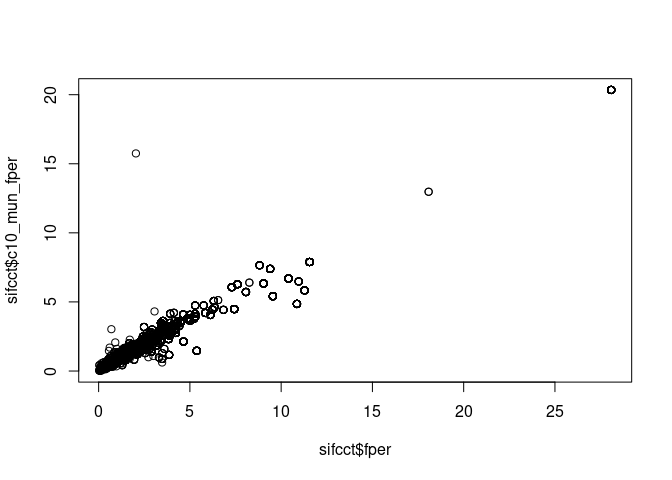
\includegraphics{analysis_1_original_mail_v5_files/figure-latex/unnamed-chunk-3-1.pdf}

\begin{Shaded}
\begin{Highlighting}[]
\KeywordTok{cor}\NormalTok{(sifcct}\OperatorTok{$}\NormalTok{fper, sifcct}\OperatorTok{$}\NormalTok{c10_mun_fper, }\DataTypeTok{use=}\StringTok{"pairwise"}\NormalTok{)}
\end{Highlighting}
\end{Shaded}

\begin{verbatim}
## [1] 0.972352
\end{verbatim}

\begin{Shaded}
\begin{Highlighting}[]
\KeywordTok{plot}\NormalTok{(sifcct}\OperatorTok{$}\NormalTok{c10_mun_fper, sifcct}\OperatorTok{$}\NormalTok{c10_sreg_fper)}
\end{Highlighting}
\end{Shaded}

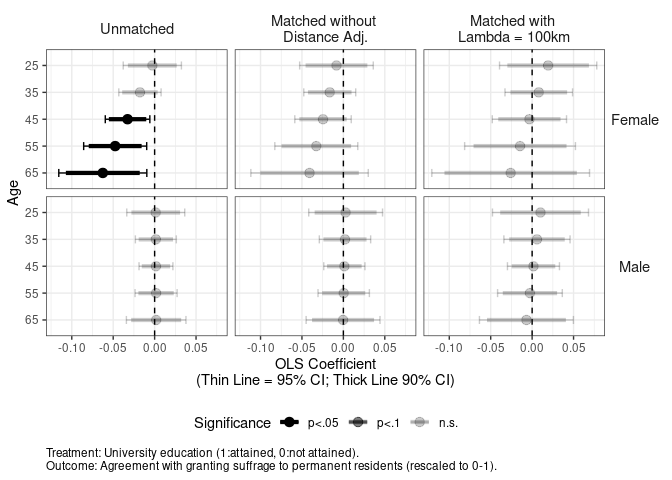
\includegraphics{analysis_1_original_mail_v5_files/figure-latex/unnamed-chunk-3-2.pdf}

\begin{Shaded}
\begin{Highlighting}[]
\KeywordTok{cor}\NormalTok{(sifcct}\OperatorTok{$}\NormalTok{c10_mun_fper, sifcct}\OperatorTok{$}\NormalTok{c10_sreg_fper, }\DataTypeTok{use=}\StringTok{"pairwise"}\NormalTok{)}
\end{Highlighting}
\end{Shaded}

\begin{verbatim}
## [1] 0.6087222
\end{verbatim}

\begin{Shaded}
\begin{Highlighting}[]
\CommentTok{## MAIL ##}

\CommentTok{## Binary Age Cohort (50s or over)}
\NormalTok{mail}\OperatorTok{$}\NormalTok{age2 <-}\StringTok{ }\KeywordTok{ifelse}\NormalTok{(mail}\OperatorTok{$}\NormalTok{age }\OperatorTok{>=}\StringTok{ }\DecValTok{50}\NormalTok{, }\DecValTok{1}\NormalTok{, }\DecValTok{0}\NormalTok{)}
\NormalTok{mail}\OperatorTok{$}\NormalTok{agex <-}\StringTok{ }\NormalTok{mail}\OperatorTok{$}\NormalTok{age}\OperatorTok{/}\DecValTok{10} \OperatorTok{-}\StringTok{ }\FloatTok{4.5}
\CommentTok{## Small Region Foreiner Percent}
\NormalTok{mail}\OperatorTok{$}\NormalTok{c10_sreg_fper <-}\StringTok{ }\NormalTok{mail}\OperatorTok{$}\NormalTok{c10_sreg_foreignN}\OperatorTok{/}\NormalTok{mail}\OperatorTok{$}\NormalTok{c10_sreg_pop}\OperatorTok{*}\DecValTok{100}
\CommentTok{## Municipality Foreigner Percent}
\NormalTok{mail}\OperatorTok{$}\NormalTok{c10_mun_fper <-}\StringTok{ }\NormalTok{mail}\OperatorTok{$}\NormalTok{c10_mun_foreignN}\OperatorTok{/}\NormalTok{mail}\OperatorTok{$}\NormalTok{c10_mun_pop}\OperatorTok{*}\DecValTok{100}
\CommentTok{## Compare Census and Foreinger Registry Numbers}
\KeywordTok{plot}\NormalTok{(mail}\OperatorTok{$}\NormalTok{fper, mail}\OperatorTok{$}\NormalTok{c10_mun_fper)}
\end{Highlighting}
\end{Shaded}

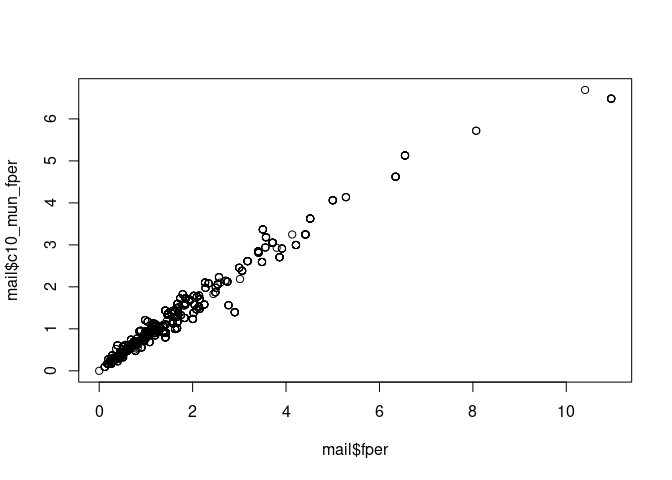
\includegraphics{analysis_1_original_mail_v5_files/figure-latex/unnamed-chunk-3-3.pdf}

\begin{Shaded}
\begin{Highlighting}[]
\KeywordTok{cor}\NormalTok{(mail}\OperatorTok{$}\NormalTok{fper, mail}\OperatorTok{$}\NormalTok{c10_mun_fper, }\DataTypeTok{use=}\StringTok{"pairwise"}\NormalTok{)}
\end{Highlighting}
\end{Shaded}

\begin{verbatim}
## [1] 0.9782127
\end{verbatim}

\begin{Shaded}
\begin{Highlighting}[]
\KeywordTok{plot}\NormalTok{(mail}\OperatorTok{$}\NormalTok{c10_mun_fper, mail}\OperatorTok{$}\NormalTok{c10_sreg_fper)}
\end{Highlighting}
\end{Shaded}

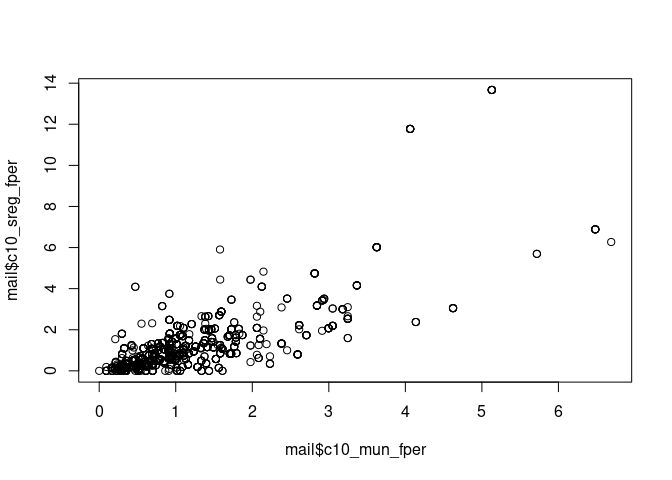
\includegraphics{analysis_1_original_mail_v5_files/figure-latex/unnamed-chunk-3-4.pdf}

\begin{Shaded}
\begin{Highlighting}[]
\KeywordTok{cor}\NormalTok{(mail}\OperatorTok{$}\NormalTok{c10_mun_fper, mail}\OperatorTok{$}\NormalTok{c10_sreg_fper, }\DataTypeTok{use=}\StringTok{"pairwise"}\NormalTok{)}
\end{Highlighting}
\end{Shaded}

\begin{verbatim}
## [1] 0.7526452
\end{verbatim}

\begin{Shaded}
\begin{Highlighting}[]
\CommentTok{## Formula (SIFCCT) ##}

\NormalTok{basemod0 <-}\StringTok{ }\KeywordTok{formula}\NormalTok{(  }\OperatorTok{~}\StringTok{ }\NormalTok{edu2}\OperatorTok{*}\NormalTok{male}\OperatorTok{*}\NormalTok{agex }\OperatorTok{+}\StringTok{ }\NormalTok{lvpr }\OperatorTok{+}\StringTok{  }
\StringTok{                        }\KeywordTok{as.factor}\NormalTok{(wave)) }\CommentTok{# sifcct}
\NormalTok{basemodA <-}\StringTok{ }\KeywordTok{formula}\NormalTok{(  }\OperatorTok{~}\StringTok{ }\NormalTok{edu2}\OperatorTok{*}\NormalTok{male}\OperatorTok{*}\NormalTok{agex }\OperatorTok{+}\StringTok{ }\NormalTok{lvpr }\OperatorTok{+}\StringTok{  }
\StringTok{                        }\NormalTok{zip_did }\OperatorTok{+}\StringTok{ }\KeywordTok{sqrt}\NormalTok{(c10_sreg_fper) }\OperatorTok{+}\StringTok{ }\KeywordTok{I}\NormalTok{(c10_sreg_edu_ugsP}\OperatorTok{/}\DecValTok{10}\NormalTok{) }\OperatorTok{+}\StringTok{ }
\StringTok{                        }\KeywordTok{as.factor}\NormalTok{(wave)) }\CommentTok{# sifcct}
\NormalTok{basemodB <-}\StringTok{ }\KeywordTok{formula}\NormalTok{(  }\OperatorTok{~}\StringTok{ }\NormalTok{edu2}\OperatorTok{*}\NormalTok{male}\OperatorTok{*}\NormalTok{agex }\OperatorTok{+}\StringTok{ }\NormalTok{lvpr }\OperatorTok{+}\StringTok{  }
\StringTok{                        }\NormalTok{didper }\OperatorTok{+}\StringTok{ }\KeywordTok{sqrt}\NormalTok{(c10_mun_fper) }\OperatorTok{+}\StringTok{ }\KeywordTok{I}\NormalTok{(c10_mun_edu_ugsP}\OperatorTok{/}\DecValTok{10}\NormalTok{) }\OperatorTok{+}\StringTok{ }
\StringTok{                        }\KeywordTok{as.factor}\NormalTok{(wave)) }\CommentTok{# sifcct}
\NormalTok{basemodC <-}\StringTok{ }\KeywordTok{formula}\NormalTok{(  }\OperatorTok{~}\StringTok{ }\NormalTok{edu2}\OperatorTok{*}\NormalTok{male}\OperatorTok{*}\NormalTok{agex }\OperatorTok{+}\StringTok{ }\NormalTok{lvpr }\OperatorTok{+}\StringTok{  }
\StringTok{                        }\NormalTok{zip_did }\OperatorTok{+}\StringTok{ }\KeywordTok{sqrt}\NormalTok{(c10_sreg_fper) }\OperatorTok{+}\StringTok{ }\KeywordTok{I}\NormalTok{(c10_sreg_edu_ugsP}\OperatorTok{/}\DecValTok{10}\NormalTok{) }\OperatorTok{+}\StringTok{ }
\StringTok{                        }\NormalTok{didper }\OperatorTok{+}\StringTok{ }\KeywordTok{sqrt}\NormalTok{(c10_mun_fper) }\OperatorTok{+}\StringTok{ }\KeywordTok{I}\NormalTok{(c10_mun_edu_ugsP}\OperatorTok{/}\DecValTok{10}\NormalTok{) }\OperatorTok{+}\StringTok{ }
\StringTok{                        }\KeywordTok{as.factor}\NormalTok{(wave)) }\CommentTok{# sifcct}

\CommentTok{## Formula (SIFCCT.mlogit) ##}

\NormalTok{outmod0.mlogit <-}\StringTok{ }\KeywordTok{Formula}\NormalTok{(foreignsuff3x  }\OperatorTok{~}\StringTok{ }\DecValTok{0} \OperatorTok{|}\StringTok{ }\NormalTok{edu2}\OperatorTok{*}\NormalTok{male}\OperatorTok{*}\NormalTok{agex }\OperatorTok{+}\StringTok{ }\NormalTok{lvpr }\OperatorTok{+}\StringTok{  }
\StringTok{                            }\KeywordTok{as.factor}\NormalTok{(wave)) }\CommentTok{# sifcct}
\NormalTok{outmodA.mlogit <-}\StringTok{ }\KeywordTok{Formula}\NormalTok{(foreignsuff3x  }\OperatorTok{~}\StringTok{ }\DecValTok{0} \OperatorTok{|}\StringTok{ }\NormalTok{edu2}\OperatorTok{*}\NormalTok{male}\OperatorTok{*}\NormalTok{agex }\OperatorTok{+}\StringTok{ }\NormalTok{lvpr }\OperatorTok{+}\StringTok{  }
\StringTok{                            }\NormalTok{zip_did }\OperatorTok{+}\StringTok{ }\KeywordTok{sqrt}\NormalTok{(c10_sreg_fper) }\OperatorTok{+}\StringTok{ }\KeywordTok{I}\NormalTok{(c10_sreg_edu_ugsP}\OperatorTok{/}\DecValTok{10}\NormalTok{) }\OperatorTok{+}\StringTok{ }
\StringTok{                            }\KeywordTok{as.factor}\NormalTok{(wave)) }\CommentTok{# sifcct}
\NormalTok{outmodB.mlogit <-}\StringTok{ }\KeywordTok{Formula}\NormalTok{(foreignsuff3x  }\OperatorTok{~}\StringTok{ }\DecValTok{0} \OperatorTok{|}\StringTok{ }\NormalTok{edu2}\OperatorTok{*}\NormalTok{male}\OperatorTok{*}\NormalTok{agex }\OperatorTok{+}\StringTok{ }\NormalTok{lvpr }\OperatorTok{+}\StringTok{  }
\StringTok{                            }\NormalTok{didper }\OperatorTok{+}\StringTok{ }\KeywordTok{sqrt}\NormalTok{(c10_mun_fper) }\OperatorTok{+}\StringTok{ }\KeywordTok{I}\NormalTok{(c10_mun_edu_ugsP}\OperatorTok{/}\DecValTok{10}\NormalTok{) }\OperatorTok{+}\StringTok{ }
\StringTok{                            }\KeywordTok{as.factor}\NormalTok{(wave)) }\CommentTok{# sifcct}
\NormalTok{outmodC.mlogit <-}\StringTok{ }\KeywordTok{Formula}\NormalTok{(foreignsuff3x  }\OperatorTok{~}\StringTok{ }\DecValTok{0} \OperatorTok{|}\StringTok{ }\NormalTok{edu2}\OperatorTok{*}\NormalTok{male}\OperatorTok{*}\NormalTok{agex }\OperatorTok{+}\StringTok{ }\NormalTok{lvpr }\OperatorTok{+}\StringTok{  }
\StringTok{                            }\NormalTok{zip_did }\OperatorTok{+}\StringTok{ }\KeywordTok{sqrt}\NormalTok{(c10_sreg_fper) }\OperatorTok{+}\StringTok{ }\KeywordTok{I}\NormalTok{(c10_sreg_edu_ugsP}\OperatorTok{/}\DecValTok{10}\NormalTok{) }\OperatorTok{+}\StringTok{ }
\StringTok{                            }\NormalTok{didper }\OperatorTok{+}\StringTok{ }\KeywordTok{sqrt}\NormalTok{(c10_mun_fper) }\OperatorTok{+}\StringTok{ }\KeywordTok{I}\NormalTok{(c10_mun_edu_ugsP}\OperatorTok{/}\DecValTok{10}\NormalTok{) }\OperatorTok{+}\StringTok{ }
\StringTok{                            }\KeywordTok{as.factor}\NormalTok{(wave)) }\CommentTok{# sifcct}

\CommentTok{## Formula (MAIL) ##}

\NormalTok{basemod0m <-}\StringTok{ }\KeywordTok{formula}\NormalTok{(  }\OperatorTok{~}\StringTok{ }\NormalTok{edu2}\OperatorTok{*}\NormalTok{male}\OperatorTok{*}\NormalTok{agex }\OperatorTok{+}\StringTok{ }\NormalTok{lvpr) }\CommentTok{# sifcct}
\NormalTok{basemodAm <-}\StringTok{ }\KeywordTok{formula}\NormalTok{(  }\OperatorTok{~}\StringTok{ }\NormalTok{edu2}\OperatorTok{*}\NormalTok{male}\OperatorTok{*}\NormalTok{agex }\OperatorTok{+}\StringTok{ }\NormalTok{lvpr }\OperatorTok{+}\StringTok{  }
\StringTok{                         }\NormalTok{zip_did }\OperatorTok{+}\StringTok{ }\KeywordTok{sqrt}\NormalTok{(c10_sreg_fper) }\OperatorTok{+}\StringTok{ }\KeywordTok{I}\NormalTok{(c10_sreg_edu_ugsP}\OperatorTok{/}\DecValTok{10}\NormalTok{)) }\CommentTok{# sifcct}
\NormalTok{basemodBm <-}\StringTok{ }\KeywordTok{formula}\NormalTok{(  }\OperatorTok{~}\StringTok{ }\NormalTok{edu2}\OperatorTok{*}\NormalTok{male}\OperatorTok{*}\NormalTok{agex }\OperatorTok{+}\StringTok{ }\NormalTok{lvpr }\OperatorTok{+}\StringTok{  }
\StringTok{                         }\NormalTok{didper }\OperatorTok{+}\StringTok{ }\KeywordTok{sqrt}\NormalTok{(c10_mun_fper) }\OperatorTok{+}\StringTok{ }\KeywordTok{I}\NormalTok{(c10_mun_edu_ugsP}\OperatorTok{/}\DecValTok{10}\NormalTok{)) }\CommentTok{# sifcct}
\NormalTok{basemodCm <-}\StringTok{ }\KeywordTok{formula}\NormalTok{(  }\OperatorTok{~}\StringTok{ }\NormalTok{edu2}\OperatorTok{*}\NormalTok{male}\OperatorTok{*}\NormalTok{agex }\OperatorTok{+}\StringTok{ }\NormalTok{lvpr }\OperatorTok{+}\StringTok{  }
\StringTok{                         }\NormalTok{zip_did }\OperatorTok{+}\StringTok{ }\KeywordTok{sqrt}\NormalTok{(c10_sreg_fper) }\OperatorTok{+}\StringTok{ }\KeywordTok{I}\NormalTok{(c10_sreg_edu_ugsP}\OperatorTok{/}\DecValTok{10}\NormalTok{) }\OperatorTok{+}\StringTok{ }
\StringTok{                         }\NormalTok{didper }\OperatorTok{+}\StringTok{ }\KeywordTok{sqrt}\NormalTok{(c10_mun_fper) }\OperatorTok{+}\StringTok{ }\KeywordTok{I}\NormalTok{(c10_mun_edu_ugsP}\OperatorTok{/}\DecValTok{10}\NormalTok{)) }\CommentTok{# sifcct}

\CommentTok{## Formula (MAIL.mlogit) ##}

\NormalTok{outmod0m.mlogit <-}\StringTok{ }\KeywordTok{Formula}\NormalTok{(foreignsuff3x  }\OperatorTok{~}\StringTok{ }\DecValTok{0} \OperatorTok{|}\StringTok{ }\NormalTok{edu2}\OperatorTok{*}\NormalTok{male}\OperatorTok{*}\NormalTok{agex }\OperatorTok{+}\StringTok{ }\NormalTok{lvpr) }\CommentTok{# sifcct}
\NormalTok{outmodAm.mlogit <-}\StringTok{ }\KeywordTok{Formula}\NormalTok{(foreignsuff3x  }\OperatorTok{~}\StringTok{ }\DecValTok{0} \OperatorTok{|}\StringTok{ }\NormalTok{edu2}\OperatorTok{*}\NormalTok{male}\OperatorTok{*}\NormalTok{agex }\OperatorTok{+}\StringTok{ }\NormalTok{lvpr }\OperatorTok{+}\StringTok{  }
\StringTok{                            }\NormalTok{zip_did }\OperatorTok{+}\StringTok{ }\KeywordTok{sqrt}\NormalTok{(c10_sreg_fper) }\OperatorTok{+}\StringTok{ }\KeywordTok{I}\NormalTok{(c10_sreg_edu_ugsP}\OperatorTok{/}\DecValTok{10}\NormalTok{)) }\CommentTok{# sifcct}
\NormalTok{outmodBm.mlogit <-}\StringTok{ }\KeywordTok{Formula}\NormalTok{(foreignsuff3x  }\OperatorTok{~}\StringTok{ }\DecValTok{0} \OperatorTok{|}\StringTok{ }\NormalTok{edu2}\OperatorTok{*}\NormalTok{male}\OperatorTok{*}\NormalTok{agex }\OperatorTok{+}\StringTok{ }\NormalTok{lvpr }\OperatorTok{+}\StringTok{  }
\StringTok{                            }\NormalTok{didper }\OperatorTok{+}\StringTok{ }\KeywordTok{sqrt}\NormalTok{(c10_mun_fper) }\OperatorTok{+}\StringTok{ }\KeywordTok{I}\NormalTok{(c10_mun_edu_ugsP}\OperatorTok{/}\DecValTok{10}\NormalTok{)) }\CommentTok{# sifcct}
\NormalTok{outmodCm.mlogit <-}\StringTok{ }\KeywordTok{Formula}\NormalTok{(foreignsuff3x  }\OperatorTok{~}\StringTok{ }\DecValTok{0} \OperatorTok{|}\StringTok{ }\NormalTok{edu2}\OperatorTok{*}\NormalTok{male}\OperatorTok{*}\NormalTok{agex }\OperatorTok{+}\StringTok{ }\NormalTok{lvpr }\OperatorTok{+}\StringTok{  }
\StringTok{                            }\NormalTok{zip_did }\OperatorTok{+}\StringTok{ }\KeywordTok{sqrt}\NormalTok{(c10_sreg_fper) }\OperatorTok{+}\StringTok{ }\KeywordTok{I}\NormalTok{(c10_sreg_edu_ugsP}\OperatorTok{/}\DecValTok{10}\NormalTok{) }\OperatorTok{+}\StringTok{ }
\StringTok{                            }\NormalTok{didper }\OperatorTok{+}\StringTok{ }\KeywordTok{sqrt}\NormalTok{(c10_mun_fper) }\OperatorTok{+}\StringTok{ }\KeywordTok{I}\NormalTok{(c10_mun_edu_ugsP}\OperatorTok{/}\DecValTok{10}\NormalTok{)) }\CommentTok{# sifcct}

\CommentTok{## Variable Names ##}

\NormalTok{vnmap <-}\StringTok{ }\KeywordTok{list}\NormalTok{(}\StringTok{"edu2"}\NormalTok{ =}\StringTok{ "University education"}\NormalTok{,}
              \StringTok{"edu2 (1)"}\NormalTok{ =}\StringTok{ "University education"}\NormalTok{,}
              \StringTok{"female"}\NormalTok{ =}\StringTok{ "Gender (female)"}\NormalTok{,}
              \StringTok{"male"}\NormalTok{ =}\StringTok{ "Gender (male)"}\NormalTok{,}
              \StringTok{"age2"}\NormalTok{ =}\StringTok{ "Age 50s or older"}\NormalTok{,}
              \StringTok{"agex"}\NormalTok{ =}\StringTok{ "Age (by 10 years, centered at 45)"}\NormalTok{,}
              \StringTok{"edu2:female"}\NormalTok{ =}\StringTok{ "University * Female"}\NormalTok{,}
              \StringTok{"edu2:male"}\NormalTok{ =}\StringTok{ "University * Male"}\NormalTok{,}
              \StringTok{"edu2 (2)"}\NormalTok{ =}\StringTok{ "University * Male"}\NormalTok{,}
              \StringTok{"edu2:age2"}\NormalTok{ =}\StringTok{ "University * >=50s"}\NormalTok{,}
              \StringTok{"edu2:agex"}\NormalTok{ =}\StringTok{ "University * Age"}\NormalTok{,}
              \StringTok{"edu2 (3)"}\NormalTok{ =}\StringTok{ "University * Age"}\NormalTok{,}
              \StringTok{"edu2:female:age2"}\NormalTok{ =}\StringTok{ "University * Female * >=50s"}\NormalTok{,}
              \StringTok{"edu2:male:age2"}\NormalTok{ =}\StringTok{ "University * Male * >=50s"}\NormalTok{,}
              \StringTok{"edu2:female:agex"}\NormalTok{ =}\StringTok{ "University * Female * Age"}\NormalTok{,}
              \StringTok{"edu2:male:agex"}\NormalTok{ =}\StringTok{ "University * Male * Age"}\NormalTok{,}
              \StringTok{"edu2 (4)"}\NormalTok{ =}\StringTok{ "University * Male * Age"}\NormalTok{,}
              \StringTok{"female:age2"}\NormalTok{ =}\StringTok{ "Female * >=50s"}\NormalTok{,}
              \StringTok{"male:age2"}\NormalTok{ =}\StringTok{ "Male * >=50s"}\NormalTok{,}
              \StringTok{"female:agex"}\NormalTok{ =}\StringTok{ "Female * Age"}\NormalTok{,}
              \StringTok{"male:agex"}\NormalTok{ =}\StringTok{ "Male * Age"}\NormalTok{,}
              \StringTok{"male (2)"}\NormalTok{ =}\StringTok{ "Male * Age"}\NormalTok{,}
              \StringTok{"agecatMiddle Aged (40-50s)"}\NormalTok{ =}\StringTok{ "Middle Aged (40-50s)"}\NormalTok{,}
              \StringTok{"agecatElder (>=60s)"}\NormalTok{ =}\StringTok{ "Elder (>=60s)"}\NormalTok{,}
              \StringTok{"lvpr"}\NormalTok{ =}\StringTok{ "% of Life Residing Locally (zip)"}\NormalTok{,}
              \StringTok{"zip_did"}\NormalTok{ =}\StringTok{ "DID residence (zip)"}\NormalTok{,}
              \StringTok{"sqrt(c10_sreg_fper)"}\NormalTok{ =}\StringTok{ "Foreigner % sqrt. (zip)"}\NormalTok{,}
              \StringTok{"c10_sreg_edu_ugsP"}\NormalTok{ =}\StringTok{ "University % (zip)"}\NormalTok{,}
              \StringTok{"I(c10_sreg_edu_ugsP/10)"}\NormalTok{ =}\StringTok{ "University % by 10% (zip)"}\NormalTok{,}
              \StringTok{"didper"}\NormalTok{ =}\StringTok{ "DID proportion (mun.)"}\NormalTok{,}
              \StringTok{"sqrt(c10_mun_fper)"}\NormalTok{ =}\StringTok{ "Foreigner % sqrt. (mun.)"}\NormalTok{,}
              \StringTok{"I(c10_mun_edu_ugsP/10)"}\NormalTok{ =}\StringTok{ "University % by 10% (mun.)"}\NormalTok{,}
              \StringTok{"c10_mun_edu_ugsP"}\NormalTok{ =}\StringTok{ "University % (mun.)"}\NormalTok{)}
\end{Highlighting}
\end{Shaded}

\hypertarget{sifcct-outcome-model}{%
\section{SIFCCT: Outcome Model}\label{sifcct-outcome-model}}

\begin{Shaded}
\begin{Highlighting}[]
\CommentTok{## Living in Local ZIP since at least age 15 ##}

\NormalTok{smo_}\DecValTok{10}\NormalTok{ <-}\StringTok{ }\KeywordTok{lm}\NormalTok{(}\KeywordTok{update}\NormalTok{(foreignsuff }\OperatorTok{~}\StringTok{ }\NormalTok{., basemod0), }\DataTypeTok{data=}\NormalTok{sifcct[}\KeywordTok{which}\NormalTok{(sifcct}\OperatorTok{$}\NormalTok{age }\OperatorTok{-}\StringTok{ }\NormalTok{sifcct}\OperatorTok{$}\NormalTok{lvlen}\OperatorTok{<=}\DecValTok{15}\NormalTok{),])}
\NormalTok{smo_1A <-}\StringTok{ }\KeywordTok{lm}\NormalTok{(}\KeywordTok{update}\NormalTok{(foreignsuff }\OperatorTok{~}\StringTok{ }\NormalTok{., basemodA), }\DataTypeTok{data=}\NormalTok{sifcct[}\KeywordTok{which}\NormalTok{(sifcct}\OperatorTok{$}\NormalTok{age }\OperatorTok{-}\StringTok{ }\NormalTok{sifcct}\OperatorTok{$}\NormalTok{lvlen}\OperatorTok{<=}\DecValTok{15}\NormalTok{),])}
\NormalTok{smo_1B <-}\StringTok{ }\KeywordTok{lm}\NormalTok{(}\KeywordTok{update}\NormalTok{(foreignsuff }\OperatorTok{~}\StringTok{ }\NormalTok{., basemodB), }\DataTypeTok{data=}\NormalTok{sifcct[}\KeywordTok{which}\NormalTok{(sifcct}\OperatorTok{$}\NormalTok{age }\OperatorTok{-}\StringTok{ }\NormalTok{sifcct}\OperatorTok{$}\NormalTok{lvlen}\OperatorTok{<=}\DecValTok{15}\NormalTok{),])}
\NormalTok{smo_1C <-}\StringTok{ }\KeywordTok{lm}\NormalTok{(}\KeywordTok{update}\NormalTok{(foreignsuff }\OperatorTok{~}\StringTok{ }\NormalTok{., basemodC), }\DataTypeTok{data=}\NormalTok{sifcct[}\KeywordTok{which}\NormalTok{(sifcct}\OperatorTok{$}\NormalTok{age }\OperatorTok{-}\StringTok{ }\NormalTok{sifcct}\OperatorTok{$}\NormalTok{lvlen}\OperatorTok{<=}\DecValTok{15}\NormalTok{),])}

\KeywordTok{screenreg}\NormalTok{(}\KeywordTok{list}\NormalTok{(smo_}\DecValTok{10}\NormalTok{,smo_1A,smo_1B,smo_1C), }\DataTypeTok{digits =} \DecValTok{4}\NormalTok{, }\CommentTok{# single.row = T,}
          \DataTypeTok{override.se =} \KeywordTok{list}\NormalTok{(}\KeywordTok{coeftest}\NormalTok{(smo_}\DecValTok{10}\NormalTok{,}\DataTypeTok{vcov.=}\KeywordTok{vcovHC}\NormalTok{(smo_}\DecValTok{10}\NormalTok{))[,}\DecValTok{2}\NormalTok{],}
                             \KeywordTok{coeftest}\NormalTok{(smo_1A,}\DataTypeTok{vcov.=}\KeywordTok{vcovHC}\NormalTok{(smo_1A))[,}\DecValTok{2}\NormalTok{],}
                             \KeywordTok{coeftest}\NormalTok{(smo_1B,}\DataTypeTok{vcov.=}\KeywordTok{vcovHC}\NormalTok{(smo_1B))[,}\DecValTok{2}\NormalTok{],}
                             \KeywordTok{coeftest}\NormalTok{(smo_1C,}\DataTypeTok{vcov.=}\KeywordTok{vcovHC}\NormalTok{(smo_1C))[,}\DecValTok{2}\NormalTok{]),}
          \DataTypeTok{override.pvalues =} \KeywordTok{list}\NormalTok{(}\KeywordTok{coeftest}\NormalTok{(smo_}\DecValTok{10}\NormalTok{,}\DataTypeTok{vcov.=}\KeywordTok{vcovHC}\NormalTok{(smo_}\DecValTok{10}\NormalTok{))[,}\DecValTok{4}\NormalTok{],}
                                  \KeywordTok{coeftest}\NormalTok{(smo_1A,}\DataTypeTok{vcov.=}\KeywordTok{vcovHC}\NormalTok{(smo_1A))[,}\DecValTok{4}\NormalTok{],}
                                  \KeywordTok{coeftest}\NormalTok{(smo_1B,}\DataTypeTok{vcov.=}\KeywordTok{vcovHC}\NormalTok{(smo_1B))[,}\DecValTok{4}\NormalTok{],}
                                  \KeywordTok{coeftest}\NormalTok{(smo_1C,}\DataTypeTok{vcov.=}\KeywordTok{vcovHC}\NormalTok{(smo_1C))[,}\DecValTok{4}\NormalTok{]),}
          \DataTypeTok{omit.coef =} \StringTok{"(wave)"}\NormalTok{,}\DataTypeTok{stars =} \KeywordTok{c}\NormalTok{(}\FloatTok{0.1}\NormalTok{,}\FloatTok{0.05}\NormalTok{,}\FloatTok{0.01}\NormalTok{,}\FloatTok{0.001}\NormalTok{), }\DataTypeTok{symbol =} \StringTok{"+"}\NormalTok{,}
          \DataTypeTok{custom.coef.map =}\NormalTok{ vnmap, }
          \DataTypeTok{custom.model.names =} \KeywordTok{c}\NormalTok{(}\StringTok{"Base"}\NormalTok{,}\StringTok{"ZIP"}\NormalTok{,}\StringTok{"Municipality"}\NormalTok{,}\StringTok{"Full"}\NormalTok{))}
\end{Highlighting}
\end{Shaded}

\begin{verbatim}
## 
## =============================================================================================
##                                    Base           ZIP            Municipality   Full         
## ---------------------------------------------------------------------------------------------
## University education                 -0.0345 *      -0.0331 *      -0.0325 *      -0.0327 *  
##                                      (0.0136)       (0.0137)       (0.0137)       (0.0137)   
## Gender (male)                        -0.1089 ***    -0.1094 ***    -0.1096 ***    -0.1097 ***
##                                      (0.0108)       (0.0108)       (0.0108)       (0.0108)   
## Age (by 10 years, centered at 45)     0.0013         0.0014         0.0014         0.0013    
##                                      (0.0057)       (0.0057)       (0.0057)       (0.0057)   
## University * Male                     0.0341 *       0.0340 *       0.0343 *       0.0343 *  
##                                      (0.0169)       (0.0170)       (0.0170)       (0.0170)   
## University * Age                     -0.0149        -0.0150        -0.0151        -0.0149    
##                                      (0.0092)       (0.0092)       (0.0092)       (0.0092)   
## University * Male * Age               0.0150         0.0151         0.0150         0.0151    
##                                      (0.0118)       (0.0118)       (0.0118)       (0.0118)   
## Male * Age                            0.0107         0.0106         0.0107         0.0106    
##                                      (0.0081)       (0.0081)       (0.0081)       (0.0081)   
## % of Life Residing Locally (zip)     -0.0356        -0.0359        -0.0358        -0.0358    
##                                      (0.0294)       (0.0295)       (0.0295)       (0.0296)   
## DID residence (zip)                                  0.0065                        0.0110    
##                                                     (0.0092)                      (0.0113)   
## Foreigner % sqrt. (zip)                             -0.0151 *                     -0.0129    
##                                                     (0.0066)                      (0.0089)   
## University % by 10% (zip)                           -0.0013                        0.0004    
##                                                     (0.0051)                      (0.0073)   
## DID proportion (mun.)                                              -0.0029        -0.0129    
##                                                                    (0.0162)       (0.0198)   
## Foreigner % sqrt. (mun.)                                           -0.0150        -0.0031    
##                                                                    (0.0093)       (0.0124)   
## University % by 10% (mun.)                                         -0.0012        -0.0012    
##                                                                    (0.0074)       (0.0103)   
## ---------------------------------------------------------------------------------------------
## R^2                                   0.0281         0.0288         0.0285         0.0289    
## Adj. R^2                              0.0246         0.0249         0.0247         0.0246    
## Num. obs.                          7827           7827           7827           7827         
## =============================================================================================
## *** p < 0.001; ** p < 0.01; * p < 0.05; + p < 0.1
\end{verbatim}

\hypertarget{sifcct-outcome-model-2}{%
\section{SIFCCT: Outcome Model 2}\label{sifcct-outcome-model-2}}

\begin{Shaded}
\begin{Highlighting}[]
\CommentTok{## Living in Local ZIP since at least age 15 ##}

\KeywordTok{require}\NormalTok{(nnet)}
\NormalTok{smo2_}\DecValTok{10}\NormalTok{ <-}\StringTok{ }\KeywordTok{multinom}\NormalTok{(}\KeywordTok{update}\NormalTok{(foreignsuff3x }\OperatorTok{~}\StringTok{ }\NormalTok{., basemod0), }\DataTypeTok{data=}\NormalTok{sifcct[}\KeywordTok{which}\NormalTok{(sifcct}\OperatorTok{$}\NormalTok{age }\OperatorTok{-}\StringTok{ }\NormalTok{sifcct}\OperatorTok{$}\NormalTok{lvlen}\OperatorTok{<=}\DecValTok{15}\NormalTok{),])}
\end{Highlighting}
\end{Shaded}

\begin{verbatim}
## # weights:  90 (58 variable)
## initial  value 8598.838383 
## iter  10 value 8276.717582
## iter  20 value 8254.943927
## iter  30 value 8249.294653
## iter  40 value 8248.353430
## final  value 8248.335241 
## converged
\end{verbatim}

\begin{Shaded}
\begin{Highlighting}[]
\NormalTok{smo2_1A <-}\StringTok{ }\KeywordTok{multinom}\NormalTok{(}\KeywordTok{update}\NormalTok{(foreignsuff3x }\OperatorTok{~}\StringTok{ }\NormalTok{., basemodA), }\DataTypeTok{data=}\NormalTok{sifcct[}\KeywordTok{which}\NormalTok{(sifcct}\OperatorTok{$}\NormalTok{age }\OperatorTok{-}\StringTok{ }\NormalTok{sifcct}\OperatorTok{$}\NormalTok{lvlen}\OperatorTok{<=}\DecValTok{15}\NormalTok{),])}
\end{Highlighting}
\end{Shaded}

\begin{verbatim}
## # weights:  99 (64 variable)
## initial  value 8598.838383 
## iter  10 value 8343.875666
## iter  20 value 8289.185217
## iter  30 value 8249.698803
## iter  40 value 8244.254566
## iter  50 value 8243.808758
## final  value 8243.793638 
## converged
\end{verbatim}

\begin{Shaded}
\begin{Highlighting}[]
\NormalTok{smo2_1B <-}\StringTok{ }\KeywordTok{multinom}\NormalTok{(}\KeywordTok{update}\NormalTok{(foreignsuff3x }\OperatorTok{~}\StringTok{ }\NormalTok{., basemodB), }\DataTypeTok{data=}\NormalTok{sifcct[}\KeywordTok{which}\NormalTok{(sifcct}\OperatorTok{$}\NormalTok{age }\OperatorTok{-}\StringTok{ }\NormalTok{sifcct}\OperatorTok{$}\NormalTok{lvlen}\OperatorTok{<=}\DecValTok{15}\NormalTok{),])}
\end{Highlighting}
\end{Shaded}

\begin{verbatim}
## # weights:  99 (64 variable)
## initial  value 8598.838383 
## iter  10 value 8345.896359
## iter  20 value 8266.970395
## iter  30 value 8249.664297
## iter  40 value 8243.592555
## iter  50 value 8243.110333
## final  value 8243.104809 
## converged
\end{verbatim}

\begin{Shaded}
\begin{Highlighting}[]
\NormalTok{smo2_1C <-}\StringTok{ }\KeywordTok{multinom}\NormalTok{(}\KeywordTok{update}\NormalTok{(foreignsuff3x }\OperatorTok{~}\StringTok{ }\NormalTok{., basemodC), }\DataTypeTok{data=}\NormalTok{sifcct[}\KeywordTok{which}\NormalTok{(sifcct}\OperatorTok{$}\NormalTok{age }\OperatorTok{-}\StringTok{ }\NormalTok{sifcct}\OperatorTok{$}\NormalTok{lvlen}\OperatorTok{<=}\DecValTok{15}\NormalTok{),])}
\end{Highlighting}
\end{Shaded}

\begin{verbatim}
## # weights:  108 (70 variable)
## initial  value 8598.838383 
## iter  10 value 8308.687907
## iter  20 value 8275.760125
## iter  30 value 8248.754268
## iter  40 value 8240.611153
## iter  50 value 8239.256612
## iter  60 value 8239.145675
## final  value 8239.143575 
## converged
\end{verbatim}

\begin{Shaded}
\begin{Highlighting}[]
\NormalTok{sifcct.mlogit <-}\StringTok{ }\KeywordTok{dfidx}\NormalTok{(sifcct[}\KeywordTok{which}\NormalTok{(sifcct}\OperatorTok{$}\NormalTok{age }\OperatorTok{-}\StringTok{ }\NormalTok{sifcct}\OperatorTok{$}\NormalTok{lvlen}\OperatorTok{<=}\DecValTok{15}\NormalTok{),],}
                       \DataTypeTok{shape =} \StringTok{"wide"}\NormalTok{, }\DataTypeTok{choice =} \StringTok{"foreignsuff3x"}\NormalTok{)}
\CommentTok{# levels(sifcct.mlogit$idx$id2) <- c("Disagree","Neither","Agree")}
\NormalTok{smo2_}\DecValTok{10}\NormalTok{ <-}\StringTok{ }\KeywordTok{mlogit}\NormalTok{(outmod0.mlogit, }\DataTypeTok{data=}\NormalTok{sifcct.mlogit, }\DataTypeTok{reflevel=}\StringTok{"Disagree"}\NormalTok{)}
\NormalTok{smo2_1A <-}\StringTok{ }\KeywordTok{mlogit}\NormalTok{(outmodA.mlogit, }\DataTypeTok{data=}\NormalTok{sifcct.mlogit, }\DataTypeTok{reflevel=}\StringTok{"Disagree"}\NormalTok{)}
\NormalTok{smo2_1B <-}\StringTok{ }\KeywordTok{mlogit}\NormalTok{(outmodB.mlogit, }\DataTypeTok{data=}\NormalTok{sifcct.mlogit, }\DataTypeTok{reflevel=}\StringTok{"Disagree"}\NormalTok{)}
\NormalTok{smo2_1C <-}\StringTok{ }\KeywordTok{mlogit}\NormalTok{(outmodC.mlogit, }\DataTypeTok{data=}\NormalTok{sifcct.mlogit, }\DataTypeTok{reflevel=}\StringTok{"Disagree"}\NormalTok{)}

\KeywordTok{screenreg}\NormalTok{(}\KeywordTok{list}\NormalTok{(smo2_}\DecValTok{10}\NormalTok{,smo2_1A), }\DataTypeTok{digits =} \DecValTok{4}\NormalTok{, }\CommentTok{# single.row = T,}
          \DataTypeTok{override.se =} \KeywordTok{list}\NormalTok{(}\KeywordTok{coeftest}\NormalTok{(smo2_}\DecValTok{10}\NormalTok{,}\DataTypeTok{vcov=}\NormalTok{sandwich)[}\KeywordTok{grep}\NormalTok{(}\StringTok{":Neither"}\NormalTok{,}\KeywordTok{names}\NormalTok{(}\KeywordTok{coef}\NormalTok{(smo2_}\DecValTok{10}\NormalTok{))),}\DecValTok{2}\NormalTok{],}
                             \KeywordTok{coeftest}\NormalTok{(smo2_}\DecValTok{10}\NormalTok{,}\DataTypeTok{vcov=}\NormalTok{sandwich)[}\KeywordTok{grep}\NormalTok{(}\StringTok{":Agree"}\NormalTok{,}\KeywordTok{names}\NormalTok{(}\KeywordTok{coef}\NormalTok{(smo2_}\DecValTok{10}\NormalTok{))),}\DecValTok{2}\NormalTok{],}
                             \KeywordTok{coeftest}\NormalTok{(smo2_1A,}\DataTypeTok{vcov=}\NormalTok{sandwich)[}\KeywordTok{grep}\NormalTok{(}\StringTok{":Neither"}\NormalTok{,}\KeywordTok{names}\NormalTok{(}\KeywordTok{coef}\NormalTok{(smo2_1A))),}\DecValTok{2}\NormalTok{],}
                             \KeywordTok{coeftest}\NormalTok{(smo2_1A,}\DataTypeTok{vcov=}\NormalTok{sandwich)[}\KeywordTok{grep}\NormalTok{(}\StringTok{":Agree"}\NormalTok{,}\KeywordTok{names}\NormalTok{(}\KeywordTok{coef}\NormalTok{(smo2_1A))),}\DecValTok{2}\NormalTok{]),}
          \DataTypeTok{override.pvalues =} \KeywordTok{list}\NormalTok{(}\KeywordTok{coeftest}\NormalTok{(smo2_}\DecValTok{10}\NormalTok{,}\DataTypeTok{vcov=}\NormalTok{sandwich)[}\KeywordTok{grep}\NormalTok{(}\StringTok{":Neither"}\NormalTok{,}\KeywordTok{names}\NormalTok{(}\KeywordTok{coef}\NormalTok{(smo2_}\DecValTok{10}\NormalTok{))),}\DecValTok{4}\NormalTok{],}
                                  \KeywordTok{coeftest}\NormalTok{(smo2_}\DecValTok{10}\NormalTok{,}\DataTypeTok{vcov=}\NormalTok{sandwich)[}\KeywordTok{grep}\NormalTok{(}\StringTok{":Agree"}\NormalTok{,}\KeywordTok{names}\NormalTok{(}\KeywordTok{coef}\NormalTok{(smo2_}\DecValTok{10}\NormalTok{))),}\DecValTok{4}\NormalTok{],}
                                  \KeywordTok{coeftest}\NormalTok{(smo2_1A,}\DataTypeTok{vcov=}\NormalTok{sandwich)[}\KeywordTok{grep}\NormalTok{(}\StringTok{":Neither"}\NormalTok{,}\KeywordTok{names}\NormalTok{(}\KeywordTok{coef}\NormalTok{(smo2_1A))),}\DecValTok{4}\NormalTok{],}
                                  \KeywordTok{coeftest}\NormalTok{(smo2_1A,}\DataTypeTok{vcov=}\NormalTok{sandwich)[}\KeywordTok{grep}\NormalTok{(}\StringTok{":Agree"}\NormalTok{,}\KeywordTok{names}\NormalTok{(}\KeywordTok{coef}\NormalTok{(smo2_1A))),}\DecValTok{4}\NormalTok{]),}
          \DataTypeTok{beside =}\NormalTok{ T,}
          \DataTypeTok{custom.coef.map =}\NormalTok{ vnmap,}
          \DataTypeTok{custom.model.names =} \KeywordTok{c}\NormalTok{(}\StringTok{"Base: Agree"}\NormalTok{,}\StringTok{"Base: Neither"}\NormalTok{,}
                                 \StringTok{"ZIP: Agree"}\NormalTok{,}\StringTok{"ZIP: Neither"}\NormalTok{),}
          \CommentTok{# custom.model.names = c("Base: Neither","Base: Agree",}
          \CommentTok{#                        "ZIP: Neither","ZIP: Agree"),}
          \DataTypeTok{omit.coef =} \StringTok{"(wave)"}\NormalTok{,}\DataTypeTok{stars =} \KeywordTok{c}\NormalTok{(}\FloatTok{0.1}\NormalTok{,}\FloatTok{0.05}\NormalTok{,}\FloatTok{0.01}\NormalTok{,}\FloatTok{0.001}\NormalTok{), }\DataTypeTok{symbol =} \StringTok{"+"}\NormalTok{)}
\end{Highlighting}
\end{Shaded}

\begin{verbatim}
## 
## ==============================================================================================
##                                    Base: Agree     Base: Neither  ZIP: Agree      ZIP: Neither
## ----------------------------------------------------------------------------------------------
## University education                  -0.2366 ***     -0.5074 *      -0.2280 ***     -0.4878 *
##                                       (0.1019)        (0.1026)       (0.1029)        (0.1034) 
## Age (by 10 years, centered at 45)      0.0267 +       -0.0845         0.0274 +       -0.0818  
##                                       (0.0447)        (0.0464)       (0.0448)        (0.0464) 
## University * Male                      0.3166 *        0.3177 *       0.3170 *        0.3198 *
##                                       (0.1256)        (0.1270)       (0.1258)        (0.1272) 
## University * Age                      -0.1114          0.0384        -0.1120          0.0358  
##                                       (0.0689)        (0.0701)       (0.0689)        (0.0701) 
## University * Male * Age                0.0813          0.0493         0.0821          0.0522  
##                                       (0.0877)        (0.0884)       (0.0877)        (0.0884) 
## Male * Age                             0.0955         -0.0154         0.0949         -0.0175  
##                                       (0.0620)        (0.0634)       (0.0620)        (0.0634) 
## % of Life Residing Locally (zip)      -0.1575          0.1758        -0.1588          0.1545  
##                                       (0.2161)        (0.2144)       (0.2174)        (0.2153) 
## DID residence (zip)                                                   0.0404          0.0117  
##                                                                      (0.0679)        (0.0677) 
## Foreigner % sqrt. (zip)                                              -0.1095 *       -0.1045 *
##                                                                      (0.0477)        (0.0494) 
## University % by 10% (zip)                                            -0.0057         -0.0319  
##                                                                      (0.0373)        (0.0370) 
## ----------------------------------------------------------------------------------------------
## AIC                                16612.6702      16612.6702     16615.5868      16615.5868  
## Log Likelihood                     -8248.3351      -8248.3351     -8243.7934      -8243.7934  
## Num. obs.                           7827            7827           7827            7827       
## K                                      3               3              3               3       
## ==============================================================================================
## *** p < 0.001; ** p < 0.01; * p < 0.05; + p < 0.1
\end{verbatim}

\begin{Shaded}
\begin{Highlighting}[]
\KeywordTok{screenreg}\NormalTok{(}\KeywordTok{list}\NormalTok{(smo2_1B,smo2_1C), }\DataTypeTok{digits =} \DecValTok{4}\NormalTok{, }\CommentTok{# single.row = T,}
          \DataTypeTok{override.se =} \KeywordTok{list}\NormalTok{(}\KeywordTok{coeftest}\NormalTok{(smo2_1B,}\DataTypeTok{vcov=}\NormalTok{sandwich)[}\KeywordTok{grep}\NormalTok{(}\StringTok{":Neither"}\NormalTok{,}\KeywordTok{names}\NormalTok{(}\KeywordTok{coef}\NormalTok{(smo2_1B))),}\DecValTok{2}\NormalTok{],}
                             \KeywordTok{coeftest}\NormalTok{(smo2_1B,}\DataTypeTok{vcov=}\NormalTok{sandwich)[}\KeywordTok{grep}\NormalTok{(}\StringTok{":Agree"}\NormalTok{,}\KeywordTok{names}\NormalTok{(}\KeywordTok{coef}\NormalTok{(smo2_1B))),}\DecValTok{2}\NormalTok{],}
                             \KeywordTok{coeftest}\NormalTok{(smo2_1C,}\DataTypeTok{vcov=}\NormalTok{sandwich)[}\KeywordTok{grep}\NormalTok{(}\StringTok{":Neither"}\NormalTok{,}\KeywordTok{names}\NormalTok{(}\KeywordTok{coef}\NormalTok{(smo2_1C))),}\DecValTok{2}\NormalTok{],}
                             \KeywordTok{coeftest}\NormalTok{(smo2_1C,}\DataTypeTok{vcov=}\NormalTok{sandwich)[}\KeywordTok{grep}\NormalTok{(}\StringTok{":Agree"}\NormalTok{,}\KeywordTok{names}\NormalTok{(}\KeywordTok{coef}\NormalTok{(smo2_1C))),}\DecValTok{2}\NormalTok{]),}
          \DataTypeTok{override.pvalues =} \KeywordTok{list}\NormalTok{(}\KeywordTok{coeftest}\NormalTok{(smo2_1B,}\DataTypeTok{vcov=}\NormalTok{sandwich)[}\KeywordTok{grep}\NormalTok{(}\StringTok{":Neither"}\NormalTok{,}\KeywordTok{names}\NormalTok{(}\KeywordTok{coef}\NormalTok{(smo2_1B))),}\DecValTok{4}\NormalTok{],}
                                  \KeywordTok{coeftest}\NormalTok{(smo2_1B,}\DataTypeTok{vcov=}\NormalTok{sandwich)[}\KeywordTok{grep}\NormalTok{(}\StringTok{":Agree"}\NormalTok{,}\KeywordTok{names}\NormalTok{(}\KeywordTok{coef}\NormalTok{(smo2_1B))),}\DecValTok{4}\NormalTok{],}
                                  \KeywordTok{coeftest}\NormalTok{(smo2_1C,}\DataTypeTok{vcov=}\NormalTok{sandwich)[}\KeywordTok{grep}\NormalTok{(}\StringTok{":Neither"}\NormalTok{,}\KeywordTok{names}\NormalTok{(}\KeywordTok{coef}\NormalTok{(smo2_1C))),}\DecValTok{4}\NormalTok{],}
                                  \KeywordTok{coeftest}\NormalTok{(smo2_1C,}\DataTypeTok{vcov=}\NormalTok{sandwich)[}\KeywordTok{grep}\NormalTok{(}\StringTok{":Agree"}\NormalTok{,}\KeywordTok{names}\NormalTok{(}\KeywordTok{coef}\NormalTok{(smo2_1C))),}\DecValTok{4}\NormalTok{]),}
          \DataTypeTok{beside =}\NormalTok{ T,}
          \CommentTok{# custom.coef.map = vnmap,}
          \DataTypeTok{custom.model.names =} \KeywordTok{c}\NormalTok{(}\StringTok{"Mun.: Agree"}\NormalTok{,}\StringTok{"Mun.: Neither"}\NormalTok{,}
                                 \StringTok{"Full: Agree"}\NormalTok{,}\StringTok{"Full: Neither"}\NormalTok{),}
          \CommentTok{# custom.model.names = c("Mun.: Neither","Mun.: Agree",}
          \CommentTok{#                        "Full: Neither","Full: Agree"),}
          \DataTypeTok{omit.coef =} \StringTok{"(wave)"}\NormalTok{,}\DataTypeTok{stars =} \KeywordTok{c}\NormalTok{(}\FloatTok{0.1}\NormalTok{,}\FloatTok{0.05}\NormalTok{,}\FloatTok{0.01}\NormalTok{,}\FloatTok{0.001}\NormalTok{), }\DataTypeTok{symbol =} \StringTok{"+"}\NormalTok{)}
\end{Highlighting}
\end{Shaded}

\begin{verbatim}
## 
## ====================================================================================
##                       Mun.: Agree     Mun.: Neither   Full: Agree     Full: Neither 
## ------------------------------------------------------------------------------------
## (Intercept)               0.2119          0.0490          0.2067          0.0595    
##                          (0.2541)        (0.2528)        (0.2545)        (0.2532)   
## edu2 (1)                 -0.2225 ***     -0.4957 *       -0.2250 ***     -0.4884 *  
##                          (0.1027)        (0.1033)        (0.1029)        (0.1036)   
## male (1)                 -0.7863 ***     -0.8100 ***     -0.7877 ***     -0.8149 ***
##                          (0.0817)        (0.0857)        (0.0819)        (0.0857)   
## agex                      0.0273 +       -0.0823          0.0267 +       -0.0816    
##                          (0.0448)        (0.0464)        (0.0448)        (0.0464)   
## lvpr                     -0.1593          0.1667         -0.1588          0.1554    
##                          (0.2175)        (0.2150)        (0.2178)        (0.2153)   
## didper                    0.0063 *       -0.2650         -0.0445 **      -0.3924    
##                          (0.1195)        (0.1198)        (0.1434)        (0.1455)   
## sqrt(c10_mun_fper)       -0.1130         -0.0532 +       -0.0283          0.0716    
##                          (0.0671)        (0.0677)        (0.0917)        (0.0929)   
## c10_mun_edu_ugsP/10      -0.0143          0.0418         -0.0233          0.1103    
##                          (0.0554)        (0.0540)        (0.0759)        (0.0746)   
## edu2 (2)                  0.3170 **       0.3288 *        0.3177 **       0.3265 *  
##                          (0.1257)        (0.1272)        (0.1258)        (0.1273)   
## edu2 (3)                 -0.1124          0.0360         -0.1117          0.0359    
##                          (0.0689)        (0.0701)        (0.0689)        (0.0701)   
## male (2)                  0.0962         -0.0180          0.0953         -0.0205    
##                          (0.0621)        (0.0634)        (0.0622)        (0.0634)   
## edu2 (4)                  0.0807          0.0515          0.0818          0.0541    
##                          (0.0877)        (0.0884)        (0.0878)        (0.0884)   
## zip_did                                                   0.0576 +        0.1353    
##                                                          (0.0821)        (0.0823)   
## sqrt(c10_sreg_fper)                                      -0.0909 *       -0.1365    
##                                                          (0.0665)        (0.0678)   
## c10_sreg_edu_ugsP/10                                      0.0115         -0.0661    
##                                                          (0.0530)        (0.0525)   
## ------------------------------------------------------------------------------------
## AIC                   16614.2088      16614.2088      16618.2864      16618.2864    
## Log Likelihood        -8243.1044      -8243.1044      -8239.1432      -8239.1432    
## Num. obs.              7827            7827            7827            7827         
## K                         3               3               3               3         
## ====================================================================================
## *** p < 0.001; ** p < 0.01; * p < 0.05; + p < 0.1
\end{verbatim}

\hypertarget{sifcct-mediator-models}{%
\section{SIFCCT: Mediator Models}\label{sifcct-mediator-models}}

\hypertarget{knowledge}{%
\subsection{Knowledge}\label{knowledge}}

\begin{Shaded}
\begin{Highlighting}[]
\NormalTok{smm01_}\DecValTok{10}\NormalTok{ <-}\StringTok{ }\KeywordTok{lm}\NormalTok{(}\KeywordTok{update}\NormalTok{(knowledge }\OperatorTok{~}\StringTok{ }\NormalTok{., basemod0), }\DataTypeTok{data=}\NormalTok{sifcct[}\KeywordTok{which}\NormalTok{(sifcct}\OperatorTok{$}\NormalTok{age }\OperatorTok{-}\StringTok{ }\NormalTok{sifcct}\OperatorTok{$}\NormalTok{lvlen}\OperatorTok{<=}\DecValTok{15}\NormalTok{),])}
\NormalTok{smm01_1A <-}\StringTok{ }\KeywordTok{lm}\NormalTok{(}\KeywordTok{update}\NormalTok{(knowledge }\OperatorTok{~}\StringTok{ }\NormalTok{., basemodA), }\DataTypeTok{data=}\NormalTok{sifcct[}\KeywordTok{which}\NormalTok{(sifcct}\OperatorTok{$}\NormalTok{age }\OperatorTok{-}\StringTok{ }\NormalTok{sifcct}\OperatorTok{$}\NormalTok{lvlen}\OperatorTok{<=}\DecValTok{15}\NormalTok{),])}
\NormalTok{smm01_1B <-}\StringTok{ }\KeywordTok{lm}\NormalTok{(}\KeywordTok{update}\NormalTok{(knowledge }\OperatorTok{~}\StringTok{ }\NormalTok{., basemodB), }\DataTypeTok{data=}\NormalTok{sifcct[}\KeywordTok{which}\NormalTok{(sifcct}\OperatorTok{$}\NormalTok{age }\OperatorTok{-}\StringTok{ }\NormalTok{sifcct}\OperatorTok{$}\NormalTok{lvlen}\OperatorTok{<=}\DecValTok{15}\NormalTok{),])}
\NormalTok{smm01_1C <-}\StringTok{ }\KeywordTok{lm}\NormalTok{(}\KeywordTok{update}\NormalTok{(knowledge }\OperatorTok{~}\StringTok{ }\NormalTok{., basemodC), }\DataTypeTok{data=}\NormalTok{sifcct[}\KeywordTok{which}\NormalTok{(sifcct}\OperatorTok{$}\NormalTok{age }\OperatorTok{-}\StringTok{ }\NormalTok{sifcct}\OperatorTok{$}\NormalTok{lvlen}\OperatorTok{<=}\DecValTok{15}\NormalTok{),])}
\KeywordTok{screenreg}\NormalTok{(}\KeywordTok{list}\NormalTok{(smm01_}\DecValTok{10}\NormalTok{,smm01_1A,smm01_1B,smm01_1C), }\DataTypeTok{digits =} \DecValTok{4}\NormalTok{, }\CommentTok{# single.row = T,}
          \DataTypeTok{override.se =} \KeywordTok{list}\NormalTok{(}\KeywordTok{coeftest}\NormalTok{(smm01_}\DecValTok{10}\NormalTok{,}\DataTypeTok{vcov.=}\KeywordTok{vcovHC}\NormalTok{(smm01_}\DecValTok{10}\NormalTok{))[,}\DecValTok{2}\NormalTok{],}
                             \KeywordTok{coeftest}\NormalTok{(smm01_1A,}\DataTypeTok{vcov.=}\KeywordTok{vcovHC}\NormalTok{(smm01_1A))[,}\DecValTok{2}\NormalTok{],}
                             \KeywordTok{coeftest}\NormalTok{(smm01_1B,}\DataTypeTok{vcov.=}\KeywordTok{vcovHC}\NormalTok{(smm01_1B))[,}\DecValTok{2}\NormalTok{],}
                             \KeywordTok{coeftest}\NormalTok{(smm01_1C,}\DataTypeTok{vcov.=}\KeywordTok{vcovHC}\NormalTok{(smm01_1C))[,}\DecValTok{2}\NormalTok{]),}
          \DataTypeTok{override.pvalues =} \KeywordTok{list}\NormalTok{(}\KeywordTok{coeftest}\NormalTok{(smm01_}\DecValTok{10}\NormalTok{,}\DataTypeTok{vcov.=}\KeywordTok{vcovHC}\NormalTok{(smm01_}\DecValTok{10}\NormalTok{))[,}\DecValTok{4}\NormalTok{],}
                                  \KeywordTok{coeftest}\NormalTok{(smm01_1A,}\DataTypeTok{vcov.=}\KeywordTok{vcovHC}\NormalTok{(smm01_1A))[,}\DecValTok{4}\NormalTok{],}
                                  \KeywordTok{coeftest}\NormalTok{(smm01_1B,}\DataTypeTok{vcov.=}\KeywordTok{vcovHC}\NormalTok{(smm01_1B))[,}\DecValTok{4}\NormalTok{],}
                                  \KeywordTok{coeftest}\NormalTok{(smm01_1C,}\DataTypeTok{vcov.=}\KeywordTok{vcovHC}\NormalTok{(smm01_1C))[,}\DecValTok{4}\NormalTok{]),}
          \DataTypeTok{omit.coef =} \StringTok{"(wave)"}\NormalTok{, }\DataTypeTok{stars =} \KeywordTok{c}\NormalTok{(}\FloatTok{0.1}\NormalTok{,}\FloatTok{0.05}\NormalTok{,}\FloatTok{0.01}\NormalTok{,}\FloatTok{0.001}\NormalTok{), }\DataTypeTok{symbol =} \StringTok{"+"}\NormalTok{,}
          \DataTypeTok{custom.coef.map =}\NormalTok{ vnmap, }
          \DataTypeTok{custom.model.names =} \KeywordTok{c}\NormalTok{(}\StringTok{"Base"}\NormalTok{,}\StringTok{"ZIP"}\NormalTok{,}\StringTok{"Municipality"}\NormalTok{,}\StringTok{"Full"}\NormalTok{))}
\end{Highlighting}
\end{Shaded}

\begin{verbatim}
## 
## =============================================================================================
##                                    Base           ZIP            Municipality   Full         
## ---------------------------------------------------------------------------------------------
## University education                  0.1553 ***     0.1483 ***     0.1510 ***     0.1486 ***
##                                      (0.0125)       (0.0126)       (0.0126)       (0.0126)   
## Gender (male)                         0.1842 ***     0.1857 ***     0.1859 ***     0.1867 ***
##                                      (0.0100)       (0.0100)       (0.0100)       (0.0100)   
## Age (by 10 years, centered at 45)     0.0542 ***     0.0536 ***     0.0540 ***     0.0537 ***
##                                      (0.0053)       (0.0053)       (0.0053)       (0.0053)   
## University * Male                    -0.0287 +      -0.0278 +      -0.0293 +      -0.0285 +  
##                                      (0.0152)       (0.0152)       (0.0152)       (0.0152)   
## University * Age                     -0.0158 +      -0.0151 +      -0.0153 +      -0.0151 +  
##                                      (0.0083)       (0.0083)       (0.0083)       (0.0083)   
## University * Male * Age               0.0054         0.0048         0.0046         0.0044    
##                                      (0.0104)       (0.0104)       (0.0104)       (0.0104)   
## Male * Age                            0.0020         0.0025         0.0025         0.0028    
##                                      (0.0074)       (0.0074)       (0.0074)       (0.0074)   
## % of Life Residing Locally (zip)     -0.1088 ***    -0.0984 ***    -0.0987 ***    -0.0961 ***
##                                      (0.0257)       (0.0257)       (0.0257)       (0.0257)   
## DID residence (zip)                                 -0.0117                       -0.0206 *  
##                                                     (0.0079)                      (0.0096)   
## Foreigner % sqrt. (zip)                             -0.0016                        0.0083    
##                                                     (0.0057)                      (0.0077)   
## University % by 10% (zip)                            0.0205 ***                    0.0178 ** 
##                                                     (0.0043)                      (0.0061)   
## DID proportion (mun.)                                               0.0052         0.0256    
##                                                                    (0.0137)       (0.0167)   
## Foreigner % sqrt. (mun.)                                           -0.0157 +      -0.0228 *  
##                                                                    (0.0081)       (0.0107)   
## University % by 10% (mun.)                                          0.0209 ***     0.0032    
##                                                                    (0.0062)       (0.0084)   
## ---------------------------------------------------------------------------------------------
## R^2                                   0.1892         0.1916         0.1912         0.1924    
## Adj. R^2                              0.1863         0.1884         0.1880         0.1888    
## Num. obs.                          7827           7827           7827           7827         
## =============================================================================================
## *** p < 0.001; ** p < 0.01; * p < 0.05; + p < 0.1
\end{verbatim}

\hypertarget{ideology}{%
\subsection{Ideology}\label{ideology}}

\begin{Shaded}
\begin{Highlighting}[]
\NormalTok{smm02_}\DecValTok{10}\NormalTok{ <-}\StringTok{ }\KeywordTok{lm}\NormalTok{(}\KeywordTok{update}\NormalTok{(ideology }\OperatorTok{~}\StringTok{ }\NormalTok{., basemod0), }\DataTypeTok{data=}\NormalTok{sifcct[}\KeywordTok{which}\NormalTok{(sifcct}\OperatorTok{$}\NormalTok{age }\OperatorTok{-}\StringTok{ }\NormalTok{sifcct}\OperatorTok{$}\NormalTok{lvlen}\OperatorTok{<=}\DecValTok{15}\NormalTok{),])}
\NormalTok{smm02_1A <-}\StringTok{ }\KeywordTok{lm}\NormalTok{(}\KeywordTok{update}\NormalTok{(ideology }\OperatorTok{~}\StringTok{ }\NormalTok{., basemodA), }\DataTypeTok{data=}\NormalTok{sifcct[}\KeywordTok{which}\NormalTok{(sifcct}\OperatorTok{$}\NormalTok{age }\OperatorTok{-}\StringTok{ }\NormalTok{sifcct}\OperatorTok{$}\NormalTok{lvlen}\OperatorTok{<=}\DecValTok{15}\NormalTok{),])}
\NormalTok{smm02_1B <-}\StringTok{ }\KeywordTok{lm}\NormalTok{(}\KeywordTok{update}\NormalTok{(ideology }\OperatorTok{~}\StringTok{ }\NormalTok{., basemodB), }\DataTypeTok{data=}\NormalTok{sifcct[}\KeywordTok{which}\NormalTok{(sifcct}\OperatorTok{$}\NormalTok{age }\OperatorTok{-}\StringTok{ }\NormalTok{sifcct}\OperatorTok{$}\NormalTok{lvlen}\OperatorTok{<=}\DecValTok{15}\NormalTok{),])}
\NormalTok{smm02_1C <-}\StringTok{ }\KeywordTok{lm}\NormalTok{(}\KeywordTok{update}\NormalTok{(ideology }\OperatorTok{~}\StringTok{ }\NormalTok{., basemodC), }\DataTypeTok{data=}\NormalTok{sifcct[}\KeywordTok{which}\NormalTok{(sifcct}\OperatorTok{$}\NormalTok{age }\OperatorTok{-}\StringTok{ }\NormalTok{sifcct}\OperatorTok{$}\NormalTok{lvlen}\OperatorTok{<=}\DecValTok{15}\NormalTok{),])}
\KeywordTok{screenreg}\NormalTok{(}\KeywordTok{list}\NormalTok{(smm02_}\DecValTok{10}\NormalTok{,smm02_1A,smm02_1B,smm02_1C), }\DataTypeTok{digits =} \DecValTok{4}\NormalTok{, }\CommentTok{# single.row = T,}
          \DataTypeTok{override.se =} \KeywordTok{list}\NormalTok{(}\KeywordTok{coeftest}\NormalTok{(smm02_}\DecValTok{10}\NormalTok{,}\DataTypeTok{vcov.=}\KeywordTok{vcovHC}\NormalTok{(smm02_}\DecValTok{10}\NormalTok{))[,}\DecValTok{2}\NormalTok{],}
                             \KeywordTok{coeftest}\NormalTok{(smm02_1A,}\DataTypeTok{vcov.=}\KeywordTok{vcovHC}\NormalTok{(smm02_1A))[,}\DecValTok{2}\NormalTok{],}
                             \KeywordTok{coeftest}\NormalTok{(smm02_1B,}\DataTypeTok{vcov.=}\KeywordTok{vcovHC}\NormalTok{(smm02_1B))[,}\DecValTok{2}\NormalTok{],}
                             \KeywordTok{coeftest}\NormalTok{(smm02_1C,}\DataTypeTok{vcov.=}\KeywordTok{vcovHC}\NormalTok{(smm02_1C))[,}\DecValTok{2}\NormalTok{]),}
          \DataTypeTok{override.pvalues =} \KeywordTok{list}\NormalTok{(}\KeywordTok{coeftest}\NormalTok{(smm02_}\DecValTok{10}\NormalTok{,}\DataTypeTok{vcov.=}\KeywordTok{vcovHC}\NormalTok{(smm02_}\DecValTok{10}\NormalTok{))[,}\DecValTok{4}\NormalTok{],}
                                  \KeywordTok{coeftest}\NormalTok{(smm02_1A,}\DataTypeTok{vcov.=}\KeywordTok{vcovHC}\NormalTok{(smm02_1A))[,}\DecValTok{4}\NormalTok{],}
                                  \KeywordTok{coeftest}\NormalTok{(smm02_1B,}\DataTypeTok{vcov.=}\KeywordTok{vcovHC}\NormalTok{(smm02_1B))[,}\DecValTok{4}\NormalTok{],}
                                  \KeywordTok{coeftest}\NormalTok{(smm02_1C,}\DataTypeTok{vcov.=}\KeywordTok{vcovHC}\NormalTok{(smm02_1C))[,}\DecValTok{4}\NormalTok{]),}
          \DataTypeTok{omit.coef =} \StringTok{"(wave)"}\NormalTok{, }\DataTypeTok{stars =} \KeywordTok{c}\NormalTok{(}\FloatTok{0.1}\NormalTok{,}\FloatTok{0.05}\NormalTok{,}\FloatTok{0.01}\NormalTok{,}\FloatTok{0.001}\NormalTok{), }\DataTypeTok{symbol =} \StringTok{"+"}\NormalTok{,}
          \DataTypeTok{custom.coef.map =}\NormalTok{ vnmap, }
          \DataTypeTok{custom.model.names =} \KeywordTok{c}\NormalTok{(}\StringTok{"Base"}\NormalTok{,}\StringTok{"ZIP"}\NormalTok{,}\StringTok{"Municipality"}\NormalTok{,}\StringTok{"Full"}\NormalTok{))}
\end{Highlighting}
\end{Shaded}

\begin{verbatim}
## 
## =============================================================================================
##                                    Base           ZIP            Municipality   Full         
## ---------------------------------------------------------------------------------------------
## University education                 -0.0120        -0.0130        -0.0127        -0.0126    
##                                      (0.0083)       (0.0083)       (0.0083)       (0.0083)   
## Gender (male)                        -0.0254 ***    -0.0251 ***    -0.0262 ***    -0.0260 ***
##                                      (0.0070)       (0.0070)       (0.0070)       (0.0070)   
## Age (by 10 years, centered at 45)    -0.0052        -0.0053        -0.0051        -0.0053    
##                                      (0.0034)       (0.0034)       (0.0034)       (0.0034)   
## University * Male                     0.0147         0.0148         0.0154         0.0152    
##                                      (0.0107)       (0.0107)       (0.0107)       (0.0107)   
## University * Age                     -0.0046        -0.0044        -0.0046        -0.0044    
##                                      (0.0055)       (0.0055)       (0.0055)       (0.0055)   
## University * Male * Age               0.0104         0.0103         0.0104         0.0102    
##                                      (0.0074)       (0.0074)       (0.0074)       (0.0074)   
## Male * Age                           -0.0003        -0.0002        -0.0004        -0.0003    
##                                      (0.0051)       (0.0051)       (0.0051)       (0.0051)   
## % of Life Residing Locally (zip)      0.0190         0.0211         0.0215         0.0223    
##                                      (0.0183)       (0.0183)       (0.0183)       (0.0184)   
## DID residence (zip)                                  0.0014                        0.0112    
##                                                     (0.0060)                      (0.0070)   
## Foreigner % sqrt. (zip)                             -0.0040                       -0.0008    
##                                                     (0.0042)                      (0.0057)   
## University % by 10% (zip)                            0.0033                        0.0004    
##                                                     (0.0033)                      (0.0045)   
## DID proportion (mun.)                                              -0.0207 +      -0.0316 *  
##                                                                    (0.0107)       (0.0125)   
## Foreigner % sqrt. (mun.)                                           -0.0067        -0.0062    
##                                                                    (0.0060)       (0.0081)   
## University % by 10% (mun.)                                          0.0104 *       0.0100    
##                                                                    (0.0048)       (0.0064)   
## ---------------------------------------------------------------------------------------------
## R^2                                   0.0054         0.0057         0.0063         0.0066    
## Adj. R^2                              0.0018         0.0017         0.0023         0.0023    
## Num. obs.                          7827           7827           7827           7827         
## =============================================================================================
## *** p < 0.001; ** p < 0.01; * p < 0.05; + p < 0.1
\end{verbatim}

\hypertarget{ldp---dpj-ft}{%
\subsection{LDP - DPJ FT}\label{ldp---dpj-ft}}

\begin{Shaded}
\begin{Highlighting}[]
\NormalTok{smm03_}\DecValTok{10}\NormalTok{ <-}\StringTok{ }\KeywordTok{lm}\NormalTok{(}\KeywordTok{update}\NormalTok{(ldpdpjft }\OperatorTok{~}\StringTok{ }\NormalTok{., basemod0), }\DataTypeTok{data=}\NormalTok{sifcct[}\KeywordTok{which}\NormalTok{(sifcct}\OperatorTok{$}\NormalTok{age }\OperatorTok{-}\StringTok{ }\NormalTok{sifcct}\OperatorTok{$}\NormalTok{lvlen}\OperatorTok{<=}\DecValTok{15}\NormalTok{),])}
\NormalTok{smm03_1A <-}\StringTok{ }\KeywordTok{lm}\NormalTok{(}\KeywordTok{update}\NormalTok{(ldpdpjft }\OperatorTok{~}\StringTok{ }\NormalTok{., basemodA), }\DataTypeTok{data=}\NormalTok{sifcct[}\KeywordTok{which}\NormalTok{(sifcct}\OperatorTok{$}\NormalTok{age }\OperatorTok{-}\StringTok{ }\NormalTok{sifcct}\OperatorTok{$}\NormalTok{lvlen}\OperatorTok{<=}\DecValTok{15}\NormalTok{),])}
\NormalTok{smm03_1B <-}\StringTok{ }\KeywordTok{lm}\NormalTok{(}\KeywordTok{update}\NormalTok{(ldpdpjft }\OperatorTok{~}\StringTok{ }\NormalTok{., basemodB), }\DataTypeTok{data=}\NormalTok{sifcct[}\KeywordTok{which}\NormalTok{(sifcct}\OperatorTok{$}\NormalTok{age }\OperatorTok{-}\StringTok{ }\NormalTok{sifcct}\OperatorTok{$}\NormalTok{lvlen}\OperatorTok{<=}\DecValTok{15}\NormalTok{),])}
\NormalTok{smm03_1C <-}\StringTok{ }\KeywordTok{lm}\NormalTok{(}\KeywordTok{update}\NormalTok{(ldpdpjft }\OperatorTok{~}\StringTok{ }\NormalTok{., basemodC), }\DataTypeTok{data=}\NormalTok{sifcct[}\KeywordTok{which}\NormalTok{(sifcct}\OperatorTok{$}\NormalTok{age }\OperatorTok{-}\StringTok{ }\NormalTok{sifcct}\OperatorTok{$}\NormalTok{lvlen}\OperatorTok{<=}\DecValTok{15}\NormalTok{),])}
\KeywordTok{screenreg}\NormalTok{(}\KeywordTok{list}\NormalTok{(smm03_}\DecValTok{10}\NormalTok{,smm03_1A,smm03_1B,smm03_1C), }\DataTypeTok{digits =} \DecValTok{4}\NormalTok{, }\CommentTok{# single.row = T,}
          \DataTypeTok{override.se =} \KeywordTok{list}\NormalTok{(}\KeywordTok{coeftest}\NormalTok{(smm03_}\DecValTok{10}\NormalTok{,}\DataTypeTok{vcov.=}\KeywordTok{vcovHC}\NormalTok{(smm03_}\DecValTok{10}\NormalTok{))[,}\DecValTok{2}\NormalTok{],}
                             \KeywordTok{coeftest}\NormalTok{(smm03_1A,}\DataTypeTok{vcov.=}\KeywordTok{vcovHC}\NormalTok{(smm03_1A))[,}\DecValTok{2}\NormalTok{],}
                             \KeywordTok{coeftest}\NormalTok{(smm03_1B,}\DataTypeTok{vcov.=}\KeywordTok{vcovHC}\NormalTok{(smm03_1B))[,}\DecValTok{2}\NormalTok{],}
                             \KeywordTok{coeftest}\NormalTok{(smm03_1C,}\DataTypeTok{vcov.=}\KeywordTok{vcovHC}\NormalTok{(smm03_1C))[,}\DecValTok{2}\NormalTok{]),}
          \DataTypeTok{override.pvalues =} \KeywordTok{list}\NormalTok{(}\KeywordTok{coeftest}\NormalTok{(smm03_}\DecValTok{10}\NormalTok{,}\DataTypeTok{vcov.=}\KeywordTok{vcovHC}\NormalTok{(smm03_}\DecValTok{10}\NormalTok{))[,}\DecValTok{4}\NormalTok{],}
                                  \KeywordTok{coeftest}\NormalTok{(smm03_1A,}\DataTypeTok{vcov.=}\KeywordTok{vcovHC}\NormalTok{(smm03_1A))[,}\DecValTok{4}\NormalTok{],}
                                  \KeywordTok{coeftest}\NormalTok{(smm03_1B,}\DataTypeTok{vcov.=}\KeywordTok{vcovHC}\NormalTok{(smm03_1B))[,}\DecValTok{4}\NormalTok{],}
                                  \KeywordTok{coeftest}\NormalTok{(smm03_1C,}\DataTypeTok{vcov.=}\KeywordTok{vcovHC}\NormalTok{(smm03_1C))[,}\DecValTok{4}\NormalTok{]),}
          \DataTypeTok{omit.coef =} \StringTok{"(wave)"}\NormalTok{, }\DataTypeTok{stars =} \KeywordTok{c}\NormalTok{(}\FloatTok{0.1}\NormalTok{,}\FloatTok{0.05}\NormalTok{,}\FloatTok{0.01}\NormalTok{,}\FloatTok{0.001}\NormalTok{), }\DataTypeTok{symbol =} \StringTok{"+"}\NormalTok{,}
          \DataTypeTok{custom.coef.map =}\NormalTok{ vnmap, }
          \DataTypeTok{custom.model.names =} \KeywordTok{c}\NormalTok{(}\StringTok{"Base"}\NormalTok{,}\StringTok{"ZIP"}\NormalTok{,}\StringTok{"Municipality"}\NormalTok{,}\StringTok{"Full"}\NormalTok{))}
\end{Highlighting}
\end{Shaded}

\begin{verbatim}
## 
## =============================================================================================
##                                    Base           ZIP            Municipality   Full         
## ---------------------------------------------------------------------------------------------
## University education                 -0.0038        -0.0045        -0.0035        -0.0042    
##                                      (0.0068)       (0.0069)       (0.0069)       (0.0069)   
## Gender (male)                         0.0220 ***     0.0222 ***     0.0216 ***     0.0220 ***
##                                      (0.0053)       (0.0054)       (0.0054)       (0.0054)   
## Age (by 10 years, centered at 45)    -0.0020        -0.0020        -0.0019        -0.0022    
##                                      (0.0028)       (0.0028)       (0.0028)       (0.0028)   
## University * Male                     0.0038         0.0039         0.0041         0.0041    
##                                      (0.0085)       (0.0086)       (0.0086)       (0.0086)   
## University * Age                     -0.0057        -0.0057        -0.0058        -0.0057    
##                                      (0.0046)       (0.0045)       (0.0046)       (0.0046)   
## University * Male * Age               0.0062         0.0062         0.0064         0.0062    
##                                      (0.0059)       (0.0059)       (0.0059)       (0.0059)   
## Male * Age                           -0.0135 ***    -0.0135 ***    -0.0137 ***    -0.0134 ***
##                                      (0.0041)       (0.0041)       (0.0041)       (0.0041)   
## % of Life Residing Locally (zip)      0.0194         0.0199         0.0178         0.0192    
##                                      (0.0142)       (0.0142)       (0.0142)       (0.0142)   
## DID residence (zip)                                 -0.0024                        0.0002    
##                                                     (0.0046)                      (0.0056)   
## Foreigner % sqrt. (zip)                              0.0042                        0.0043    
##                                                     (0.0033)                      (0.0044)   
## University % by 10% (zip)                            0.0012                        0.0058 +  
##                                                     (0.0025)                      (0.0035)   
## DID proportion (mun.)                                              -0.0055        -0.0057    
##                                                                    (0.0081)       (0.0098)   
## Foreigner % sqrt. (mun.)                                            0.0059         0.0020    
##                                                                    (0.0047)       (0.0062)   
## University % by 10% (mun.)                                         -0.0019        -0.0078    
##                                                                    (0.0038)       (0.0051)   
## ---------------------------------------------------------------------------------------------
## R^2                                   0.0989         0.0991         0.0992         0.0996    
## Adj. R^2                              0.0956         0.0955         0.0956         0.0957    
## Num. obs.                          7827           7827           7827           7827         
## =============================================================================================
## *** p < 0.001; ** p < 0.01; * p < 0.05; + p < 0.1
\end{verbatim}

\hypertarget{favorability-of-south-korea}{%
\subsection{Favorability of South
Korea}\label{favorability-of-south-korea}}

\begin{Shaded}
\begin{Highlighting}[]
\NormalTok{smm04_}\DecValTok{10}\NormalTok{ <-}\StringTok{ }\KeywordTok{lm}\NormalTok{(}\KeywordTok{update}\NormalTok{(familiarityFT_KOR }\OperatorTok{~}\StringTok{ }\NormalTok{., basemod0), }\DataTypeTok{data=}\NormalTok{sifcct[}\KeywordTok{which}\NormalTok{(sifcct}\OperatorTok{$}\NormalTok{age }\OperatorTok{-}\StringTok{ }\NormalTok{sifcct}\OperatorTok{$}\NormalTok{lvlen}\OperatorTok{<=}\DecValTok{15}\NormalTok{),])}
\NormalTok{smm04_1A <-}\StringTok{ }\KeywordTok{lm}\NormalTok{(}\KeywordTok{update}\NormalTok{(familiarityFT_KOR }\OperatorTok{~}\StringTok{ }\NormalTok{., basemodA), }\DataTypeTok{data=}\NormalTok{sifcct[}\KeywordTok{which}\NormalTok{(sifcct}\OperatorTok{$}\NormalTok{age }\OperatorTok{-}\StringTok{ }\NormalTok{sifcct}\OperatorTok{$}\NormalTok{lvlen}\OperatorTok{<=}\DecValTok{15}\NormalTok{),])}
\NormalTok{smm04_1B <-}\StringTok{ }\KeywordTok{lm}\NormalTok{(}\KeywordTok{update}\NormalTok{(familiarityFT_KOR }\OperatorTok{~}\StringTok{ }\NormalTok{., basemodB), }\DataTypeTok{data=}\NormalTok{sifcct[}\KeywordTok{which}\NormalTok{(sifcct}\OperatorTok{$}\NormalTok{age }\OperatorTok{-}\StringTok{ }\NormalTok{sifcct}\OperatorTok{$}\NormalTok{lvlen}\OperatorTok{<=}\DecValTok{15}\NormalTok{),])}
\NormalTok{smm04_1C <-}\StringTok{ }\KeywordTok{lm}\NormalTok{(}\KeywordTok{update}\NormalTok{(familiarityFT_KOR }\OperatorTok{~}\StringTok{ }\NormalTok{., basemodC), }\DataTypeTok{data=}\NormalTok{sifcct[}\KeywordTok{which}\NormalTok{(sifcct}\OperatorTok{$}\NormalTok{age }\OperatorTok{-}\StringTok{ }\NormalTok{sifcct}\OperatorTok{$}\NormalTok{lvlen}\OperatorTok{<=}\DecValTok{15}\NormalTok{),])}
\KeywordTok{screenreg}\NormalTok{(}\KeywordTok{list}\NormalTok{(smm04_}\DecValTok{10}\NormalTok{,smm04_1A,smm04_1B,smm04_1C), }\DataTypeTok{digits =} \DecValTok{4}\NormalTok{, }\CommentTok{# single.row = T,}
          \DataTypeTok{override.se =} \KeywordTok{list}\NormalTok{(}\KeywordTok{coeftest}\NormalTok{(smm04_}\DecValTok{10}\NormalTok{,}\DataTypeTok{vcov.=}\KeywordTok{vcovHC}\NormalTok{(smm04_}\DecValTok{10}\NormalTok{))[,}\DecValTok{2}\NormalTok{],}
                             \KeywordTok{coeftest}\NormalTok{(smm04_1A,}\DataTypeTok{vcov.=}\KeywordTok{vcovHC}\NormalTok{(smm04_1A))[,}\DecValTok{2}\NormalTok{],}
                             \KeywordTok{coeftest}\NormalTok{(smm04_1B,}\DataTypeTok{vcov.=}\KeywordTok{vcovHC}\NormalTok{(smm04_1B))[,}\DecValTok{2}\NormalTok{],}
                             \KeywordTok{coeftest}\NormalTok{(smm04_1C,}\DataTypeTok{vcov.=}\KeywordTok{vcovHC}\NormalTok{(smm04_1C))[,}\DecValTok{2}\NormalTok{]),}
          \DataTypeTok{override.pvalues =} \KeywordTok{list}\NormalTok{(}\KeywordTok{coeftest}\NormalTok{(smm04_}\DecValTok{10}\NormalTok{,}\DataTypeTok{vcov.=}\KeywordTok{vcovHC}\NormalTok{(smm04_}\DecValTok{10}\NormalTok{))[,}\DecValTok{4}\NormalTok{],}
                                  \KeywordTok{coeftest}\NormalTok{(smm04_1A,}\DataTypeTok{vcov.=}\KeywordTok{vcovHC}\NormalTok{(smm04_1A))[,}\DecValTok{4}\NormalTok{],}
                                  \KeywordTok{coeftest}\NormalTok{(smm04_1B,}\DataTypeTok{vcov.=}\KeywordTok{vcovHC}\NormalTok{(smm04_1B))[,}\DecValTok{4}\NormalTok{],}
                                  \KeywordTok{coeftest}\NormalTok{(smm04_1C,}\DataTypeTok{vcov.=}\KeywordTok{vcovHC}\NormalTok{(smm04_1C))[,}\DecValTok{4}\NormalTok{]),}
          \DataTypeTok{omit.coef =} \StringTok{"(wave)"}\NormalTok{, }\DataTypeTok{stars =} \KeywordTok{c}\NormalTok{(}\FloatTok{0.1}\NormalTok{,}\FloatTok{0.05}\NormalTok{,}\FloatTok{0.01}\NormalTok{,}\FloatTok{0.001}\NormalTok{), }\DataTypeTok{symbol =} \StringTok{"+"}\NormalTok{,}
          \DataTypeTok{custom.coef.map =}\NormalTok{ vnmap, }
          \DataTypeTok{custom.model.names =} \KeywordTok{c}\NormalTok{(}\StringTok{"Base"}\NormalTok{,}\StringTok{"ZIP"}\NormalTok{,}\StringTok{"Municipality"}\NormalTok{,}\StringTok{"Full"}\NormalTok{))}
\end{Highlighting}
\end{Shaded}

\begin{verbatim}
## 
## =============================================================================================
##                                    Base           ZIP            Municipality   Full         
## ---------------------------------------------------------------------------------------------
## University education                 -0.0088        -0.0106        -0.0107        -0.0113    
##                                      (0.0104)       (0.0105)       (0.0105)       (0.0105)   
## Gender (male)                        -0.0580 ***    -0.0581 ***    -0.0578 ***    -0.0580 ***
##                                      (0.0083)       (0.0083)       (0.0083)       (0.0084)   
## Age (by 10 years, centered at 45)     0.0094 *       0.0094 *       0.0093 *       0.0096 *  
##                                      (0.0046)       (0.0046)       (0.0046)       (0.0046)   
## University * Male                     0.0153         0.0159         0.0155         0.0159    
##                                      (0.0127)       (0.0127)       (0.0127)       (0.0127)   
## University * Age                     -0.0141 +      -0.0141 *      -0.0140 +      -0.0142 *  
##                                      (0.0072)       (0.0072)       (0.0072)       (0.0072)   
## University * Male * Age               0.0073         0.0073         0.0073         0.0075    
##                                      (0.0090)       (0.0090)       (0.0090)       (0.0090)   
## Male * Age                            0.0190 **      0.0190 **      0.0189 **      0.0188 ** 
##                                      (0.0063)       (0.0063)       (0.0063)       (0.0063)   
## % of Life Residing Locally (zip)     -0.0103        -0.0087        -0.0088        -0.0096    
##                                      (0.0227)       (0.0227)       (0.0227)       (0.0227)   
## DID residence (zip)                                 -0.0109                       -0.0127    
##                                                     (0.0068)                      (0.0082)   
## Foreigner % sqrt. (zip)                              0.0030                       -0.0037    
##                                                     (0.0047)                      (0.0065)   
## University % by 10% (zip)                            0.0055                        0.0023    
##                                                     (0.0038)                      (0.0053)   
## DID proportion (mun.)                                              -0.0084         0.0044    
##                                                                    (0.0118)       (0.0143)   
## Foreigner % sqrt. (mun.)                                            0.0086         0.0124    
##                                                                    (0.0068)       (0.0092)   
## University % by 10% (mun.)                                          0.0063         0.0042    
##                                                                    (0.0056)       (0.0076)   
## ---------------------------------------------------------------------------------------------
## R^2                                   0.0740         0.0744         0.0744         0.0747    
## Adj. R^2                              0.0706         0.0707         0.0707         0.0707    
## Num. obs.                          7827           7827           7827           7827         
## =============================================================================================
## *** p < 0.001; ** p < 0.01; * p < 0.05; + p < 0.1
\end{verbatim}

\hypertarget{favorability-of-china}{%
\subsection{Favorability of China}\label{favorability-of-china}}

\begin{Shaded}
\begin{Highlighting}[]
\NormalTok{smm05_}\DecValTok{10}\NormalTok{ <-}\StringTok{ }\KeywordTok{lm}\NormalTok{(}\KeywordTok{update}\NormalTok{(familiarityFT_CHN }\OperatorTok{~}\StringTok{ }\NormalTok{., basemod0), }\DataTypeTok{data=}\NormalTok{sifcct[}\KeywordTok{which}\NormalTok{(sifcct}\OperatorTok{$}\NormalTok{age }\OperatorTok{-}\StringTok{ }\NormalTok{sifcct}\OperatorTok{$}\NormalTok{lvlen}\OperatorTok{<=}\DecValTok{15}\NormalTok{),])}
\NormalTok{smm05_1A <-}\StringTok{ }\KeywordTok{lm}\NormalTok{(}\KeywordTok{update}\NormalTok{(familiarityFT_CHN }\OperatorTok{~}\StringTok{ }\NormalTok{., basemodA), }\DataTypeTok{data=}\NormalTok{sifcct[}\KeywordTok{which}\NormalTok{(sifcct}\OperatorTok{$}\NormalTok{age }\OperatorTok{-}\StringTok{ }\NormalTok{sifcct}\OperatorTok{$}\NormalTok{lvlen}\OperatorTok{<=}\DecValTok{15}\NormalTok{),])}
\NormalTok{smm05_1B <-}\StringTok{ }\KeywordTok{lm}\NormalTok{(}\KeywordTok{update}\NormalTok{(familiarityFT_CHN }\OperatorTok{~}\StringTok{ }\NormalTok{., basemodB), }\DataTypeTok{data=}\NormalTok{sifcct[}\KeywordTok{which}\NormalTok{(sifcct}\OperatorTok{$}\NormalTok{age }\OperatorTok{-}\StringTok{ }\NormalTok{sifcct}\OperatorTok{$}\NormalTok{lvlen}\OperatorTok{<=}\DecValTok{15}\NormalTok{),])}
\NormalTok{smm05_1C <-}\StringTok{ }\KeywordTok{lm}\NormalTok{(}\KeywordTok{update}\NormalTok{(familiarityFT_CHN }\OperatorTok{~}\StringTok{ }\NormalTok{., basemodC), }\DataTypeTok{data=}\NormalTok{sifcct[}\KeywordTok{which}\NormalTok{(sifcct}\OperatorTok{$}\NormalTok{age }\OperatorTok{-}\StringTok{ }\NormalTok{sifcct}\OperatorTok{$}\NormalTok{lvlen}\OperatorTok{<=}\DecValTok{15}\NormalTok{),])}
\KeywordTok{screenreg}\NormalTok{(}\KeywordTok{list}\NormalTok{(smm05_}\DecValTok{10}\NormalTok{,smm05_1A,smm05_1B,smm05_1C), }\DataTypeTok{digits =} \DecValTok{4}\NormalTok{, }\CommentTok{# single.row = T,}
          \DataTypeTok{override.se =} \KeywordTok{list}\NormalTok{(}\KeywordTok{coeftest}\NormalTok{(smm05_}\DecValTok{10}\NormalTok{,}\DataTypeTok{vcov.=}\KeywordTok{vcovHC}\NormalTok{(smm05_}\DecValTok{10}\NormalTok{))[,}\DecValTok{2}\NormalTok{],}
                             \KeywordTok{coeftest}\NormalTok{(smm05_1A,}\DataTypeTok{vcov.=}\KeywordTok{vcovHC}\NormalTok{(smm05_1A))[,}\DecValTok{2}\NormalTok{],}
                             \KeywordTok{coeftest}\NormalTok{(smm05_1B,}\DataTypeTok{vcov.=}\KeywordTok{vcovHC}\NormalTok{(smm05_1B))[,}\DecValTok{2}\NormalTok{],}
                             \KeywordTok{coeftest}\NormalTok{(smm05_1C,}\DataTypeTok{vcov.=}\KeywordTok{vcovHC}\NormalTok{(smm05_1C))[,}\DecValTok{2}\NormalTok{]),}
          \DataTypeTok{override.pvalues =} \KeywordTok{list}\NormalTok{(}\KeywordTok{coeftest}\NormalTok{(smm05_}\DecValTok{10}\NormalTok{,}\DataTypeTok{vcov.=}\KeywordTok{vcovHC}\NormalTok{(smm05_}\DecValTok{10}\NormalTok{))[,}\DecValTok{4}\NormalTok{],}
                                  \KeywordTok{coeftest}\NormalTok{(smm05_1A,}\DataTypeTok{vcov.=}\KeywordTok{vcovHC}\NormalTok{(smm05_1A))[,}\DecValTok{4}\NormalTok{],}
                                  \KeywordTok{coeftest}\NormalTok{(smm05_1B,}\DataTypeTok{vcov.=}\KeywordTok{vcovHC}\NormalTok{(smm05_1B))[,}\DecValTok{4}\NormalTok{],}
                                  \KeywordTok{coeftest}\NormalTok{(smm05_1C,}\DataTypeTok{vcov.=}\KeywordTok{vcovHC}\NormalTok{(smm05_1C))[,}\DecValTok{4}\NormalTok{]),}
          \DataTypeTok{omit.coef =} \StringTok{"(wave)"}\NormalTok{, }\DataTypeTok{stars =} \KeywordTok{c}\NormalTok{(}\FloatTok{0.1}\NormalTok{,}\FloatTok{0.05}\NormalTok{,}\FloatTok{0.01}\NormalTok{,}\FloatTok{0.001}\NormalTok{), }\DataTypeTok{symbol =} \StringTok{"+"}\NormalTok{,}
          \DataTypeTok{custom.coef.map =}\NormalTok{ vnmap, }
          \DataTypeTok{custom.model.names =} \KeywordTok{c}\NormalTok{(}\StringTok{"Base"}\NormalTok{,}\StringTok{"ZIP"}\NormalTok{,}\StringTok{"Municipality"}\NormalTok{,}\StringTok{"Full"}\NormalTok{))}
\end{Highlighting}
\end{Shaded}

\begin{verbatim}
## 
## =========================================================================================
##                                    Base          ZIP           Municipality  Full        
## -----------------------------------------------------------------------------------------
## University education                 -0.0055       -0.0052       -0.0053       -0.0053   
##                                      (0.0088)      (0.0089)      (0.0089)      (0.0089)  
## Gender (male)                        -0.0185 **    -0.0192 **    -0.0195 **    -0.0197 **
##                                      (0.0072)      (0.0072)      (0.0072)      (0.0072)  
## Age (by 10 years, centered at 45)    -0.0051       -0.0049       -0.0050       -0.0049   
##                                      (0.0041)      (0.0041)      (0.0041)      (0.0041)  
## University * Male                     0.0131        0.0136        0.0138        0.0139   
##                                      (0.0108)      (0.0108)      (0.0108)      (0.0108)  
## University * Age                     -0.0122 *     -0.0124 *     -0.0124 *     -0.0124 * 
##                                      (0.0062)      (0.0062)      (0.0062)      (0.0062)  
## University * Male * Age               0.0043        0.0045        0.0045        0.0046   
##                                      (0.0078)      (0.0078)      (0.0078)      (0.0078)  
## Male * Age                            0.0071        0.0070        0.0069        0.0068   
##                                      (0.0056)      (0.0056)      (0.0056)      (0.0056)  
## % of Life Residing Locally (zip)     -0.0446 *     -0.0454 *     -0.0449 *     -0.0456 * 
##                                      (0.0195)      (0.0195)      (0.0195)      (0.0195)  
## DID residence (zip)                                -0.0060                     -0.0006   
##                                                    (0.0058)                    (0.0069)  
## Foreigner % sqrt. (zip)                            -0.0044                     -0.0072   
##                                                    (0.0041)                    (0.0056)  
## University % by 10% (zip)                           0.0008                     -0.0009   
##                                                    (0.0032)                    (0.0045)  
## DID proportion (mun.)                                            -0.0182 +     -0.0173   
##                                                                  (0.0102)      (0.0122)  
## Foreigner % sqrt. (mun.)                                         -0.0008        0.0060   
##                                                                  (0.0057)      (0.0077)  
## University % by 10% (mun.)                                        0.0039        0.0050   
##                                                                  (0.0047)      (0.0065)  
## -----------------------------------------------------------------------------------------
## R^2                                   0.0332        0.0336        0.0337        0.0339   
## Adj. R^2                              0.0298        0.0297        0.0298        0.0297   
## Num. obs.                          7827          7827          7827          7827        
## =========================================================================================
## *** p < 0.001; ** p < 0.01; * p < 0.05; + p < 0.1
\end{verbatim}

\hypertarget{favorability-of-usa}{%
\subsection{Favorability of USA}\label{favorability-of-usa}}

\begin{Shaded}
\begin{Highlighting}[]
\NormalTok{smm06_}\DecValTok{10}\NormalTok{ <-}\StringTok{ }\KeywordTok{lm}\NormalTok{(}\KeywordTok{update}\NormalTok{(familiarityFT_USA }\OperatorTok{~}\StringTok{ }\NormalTok{., basemod0), }\DataTypeTok{data=}\NormalTok{sifcct[}\KeywordTok{which}\NormalTok{(sifcct}\OperatorTok{$}\NormalTok{age }\OperatorTok{-}\StringTok{ }\NormalTok{sifcct}\OperatorTok{$}\NormalTok{lvlen}\OperatorTok{<=}\DecValTok{15}\NormalTok{),])}
\NormalTok{smm06_1A <-}\StringTok{ }\KeywordTok{lm}\NormalTok{(}\KeywordTok{update}\NormalTok{(familiarityFT_USA }\OperatorTok{~}\StringTok{ }\NormalTok{., basemodA), }\DataTypeTok{data=}\NormalTok{sifcct[}\KeywordTok{which}\NormalTok{(sifcct}\OperatorTok{$}\NormalTok{age }\OperatorTok{-}\StringTok{ }\NormalTok{sifcct}\OperatorTok{$}\NormalTok{lvlen}\OperatorTok{<=}\DecValTok{15}\NormalTok{),])}
\NormalTok{smm06_1B <-}\StringTok{ }\KeywordTok{lm}\NormalTok{(}\KeywordTok{update}\NormalTok{(familiarityFT_USA }\OperatorTok{~}\StringTok{ }\NormalTok{., basemodB), }\DataTypeTok{data=}\NormalTok{sifcct[}\KeywordTok{which}\NormalTok{(sifcct}\OperatorTok{$}\NormalTok{age }\OperatorTok{-}\StringTok{ }\NormalTok{sifcct}\OperatorTok{$}\NormalTok{lvlen}\OperatorTok{<=}\DecValTok{15}\NormalTok{),])}
\NormalTok{smm06_1C <-}\StringTok{ }\KeywordTok{lm}\NormalTok{(}\KeywordTok{update}\NormalTok{(familiarityFT_USA }\OperatorTok{~}\StringTok{ }\NormalTok{., basemodC), }\DataTypeTok{data=}\NormalTok{sifcct[}\KeywordTok{which}\NormalTok{(sifcct}\OperatorTok{$}\NormalTok{age }\OperatorTok{-}\StringTok{ }\NormalTok{sifcct}\OperatorTok{$}\NormalTok{lvlen}\OperatorTok{<=}\DecValTok{15}\NormalTok{),])}
\KeywordTok{screenreg}\NormalTok{(}\KeywordTok{list}\NormalTok{(smm06_}\DecValTok{10}\NormalTok{,smm06_1A,smm06_1B,smm06_1C), }\DataTypeTok{digits =} \DecValTok{4}\NormalTok{, }\CommentTok{# single.row = T,}
          \DataTypeTok{override.se =} \KeywordTok{list}\NormalTok{(}\KeywordTok{coeftest}\NormalTok{(smm06_}\DecValTok{10}\NormalTok{,}\DataTypeTok{vcov.=}\KeywordTok{vcovHC}\NormalTok{(smm06_}\DecValTok{10}\NormalTok{))[,}\DecValTok{2}\NormalTok{],}
                             \KeywordTok{coeftest}\NormalTok{(smm06_1A,}\DataTypeTok{vcov.=}\KeywordTok{vcovHC}\NormalTok{(smm06_1A))[,}\DecValTok{2}\NormalTok{],}
                             \KeywordTok{coeftest}\NormalTok{(smm06_1B,}\DataTypeTok{vcov.=}\KeywordTok{vcovHC}\NormalTok{(smm06_1B))[,}\DecValTok{2}\NormalTok{],}
                             \KeywordTok{coeftest}\NormalTok{(smm06_1C,}\DataTypeTok{vcov.=}\KeywordTok{vcovHC}\NormalTok{(smm06_1C))[,}\DecValTok{2}\NormalTok{]),}
          \DataTypeTok{override.pvalues =} \KeywordTok{list}\NormalTok{(}\KeywordTok{coeftest}\NormalTok{(smm06_}\DecValTok{10}\NormalTok{,}\DataTypeTok{vcov.=}\KeywordTok{vcovHC}\NormalTok{(smm06_}\DecValTok{10}\NormalTok{))[,}\DecValTok{4}\NormalTok{],}
                                  \KeywordTok{coeftest}\NormalTok{(smm06_1A,}\DataTypeTok{vcov.=}\KeywordTok{vcovHC}\NormalTok{(smm06_1A))[,}\DecValTok{4}\NormalTok{],}
                                  \KeywordTok{coeftest}\NormalTok{(smm06_1B,}\DataTypeTok{vcov.=}\KeywordTok{vcovHC}\NormalTok{(smm06_1B))[,}\DecValTok{4}\NormalTok{],}
                                  \KeywordTok{coeftest}\NormalTok{(smm06_1C,}\DataTypeTok{vcov.=}\KeywordTok{vcovHC}\NormalTok{(smm06_1C))[,}\DecValTok{4}\NormalTok{]),}
          \DataTypeTok{omit.coef =} \StringTok{"(wave)"}\NormalTok{, }\DataTypeTok{stars =} \KeywordTok{c}\NormalTok{(}\FloatTok{0.1}\NormalTok{,}\FloatTok{0.05}\NormalTok{,}\FloatTok{0.01}\NormalTok{,}\FloatTok{0.001}\NormalTok{), }\DataTypeTok{symbol =} \StringTok{"+"}\NormalTok{,}
          \DataTypeTok{custom.coef.map =}\NormalTok{ vnmap, }
          \DataTypeTok{custom.model.names =} \KeywordTok{c}\NormalTok{(}\StringTok{"Base"}\NormalTok{,}\StringTok{"ZIP"}\NormalTok{,}\StringTok{"Municipality"}\NormalTok{,}\StringTok{"Full"}\NormalTok{))}
\end{Highlighting}
\end{Shaded}

\begin{verbatim}
## 
## =============================================================================================
##                                    Base           ZIP            Municipality   Full         
## ---------------------------------------------------------------------------------------------
## University education                 -0.0085        -0.0102        -0.0108        -0.0111    
##                                      (0.0090)       (0.0091)       (0.0091)       (0.0091)   
## Gender (male)                         0.0263 ***     0.0268 ***     0.0274 ***     0.0271 ***
##                                      (0.0073)       (0.0073)       (0.0073)       (0.0073)   
## Age (by 10 years, centered at 45)     0.0066 +       0.0064         0.0065 +       0.0067 +  
##                                      (0.0039)       (0.0039)       (0.0039)       (0.0039)   
## University * Male                     0.0211 +       0.0212 +       0.0207 +       0.0210 +  
##                                      (0.0112)       (0.0112)       (0.0112)       (0.0112)   
## University * Age                     -0.0136 *      -0.0133 *      -0.0133 *      -0.0134 *  
##                                      (0.0061)       (0.0061)       (0.0061)       (0.0061)   
## University * Male * Age               0.0134 +       0.0133 +       0.0132 +       0.0135 +  
##                                      (0.0078)       (0.0078)       (0.0078)       (0.0078)   
## Male * Age                            0.0043         0.0044         0.0044         0.0042    
##                                      (0.0055)       (0.0055)       (0.0055)       (0.0055)   
## % of Life Residing Locally (zip)     -0.0302        -0.0271        -0.0268        -0.0277    
##                                      (0.0192)       (0.0193)       (0.0193)       (0.0194)   
## DID residence (zip)                                 -0.0002                       -0.0048    
##                                                     (0.0060)                      (0.0071)   
## Foreigner % sqrt. (zip)                             -0.0032                       -0.0100 +  
##                                                     (0.0042)                      (0.0058)   
## University % by 10% (zip)                            0.0054                        0.0005    
##                                                     (0.0034)                      (0.0048)   
## DID proportion (mun.)                                               0.0068         0.0121    
##                                                                    (0.0107)       (0.0127)   
## Foreigner % sqrt. (mun.)                                            0.0018         0.0113    
##                                                                    (0.0060)       (0.0080)   
## University % by 10% (mun.)                                          0.0065         0.0063    
##                                                                    (0.0050)       (0.0068)   
## ---------------------------------------------------------------------------------------------
## R^2                                   0.0230         0.0235         0.0238         0.0243    
## Adj. R^2                              0.0195         0.0196         0.0199         0.0200    
## Num. obs.                          7827           7827           7827           7827         
## =============================================================================================
## *** p < 0.001; ** p < 0.01; * p < 0.05; + p < 0.1
\end{verbatim}

\hypertarget{income}{%
\subsection{Income}\label{income}}

\begin{Shaded}
\begin{Highlighting}[]
\NormalTok{smm07_}\DecValTok{10}\NormalTok{ <-}\StringTok{ }\KeywordTok{lm}\NormalTok{(}\KeywordTok{update}\NormalTok{(income }\OperatorTok{~}\StringTok{ }\NormalTok{., basemod0), }\DataTypeTok{data=}\NormalTok{sifcct[}\KeywordTok{which}\NormalTok{(sifcct}\OperatorTok{$}\NormalTok{age }\OperatorTok{-}\StringTok{ }\NormalTok{sifcct}\OperatorTok{$}\NormalTok{lvlen}\OperatorTok{<=}\DecValTok{15}\NormalTok{),])}
\NormalTok{smm07_1A <-}\StringTok{ }\KeywordTok{lm}\NormalTok{(}\KeywordTok{update}\NormalTok{(income }\OperatorTok{~}\StringTok{ }\NormalTok{., basemodA), }\DataTypeTok{data=}\NormalTok{sifcct[}\KeywordTok{which}\NormalTok{(sifcct}\OperatorTok{$}\NormalTok{age }\OperatorTok{-}\StringTok{ }\NormalTok{sifcct}\OperatorTok{$}\NormalTok{lvlen}\OperatorTok{<=}\DecValTok{15}\NormalTok{),])}
\NormalTok{smm07_1B <-}\StringTok{ }\KeywordTok{lm}\NormalTok{(}\KeywordTok{update}\NormalTok{(income }\OperatorTok{~}\StringTok{ }\NormalTok{., basemodB), }\DataTypeTok{data=}\NormalTok{sifcct[}\KeywordTok{which}\NormalTok{(sifcct}\OperatorTok{$}\NormalTok{age }\OperatorTok{-}\StringTok{ }\NormalTok{sifcct}\OperatorTok{$}\NormalTok{lvlen}\OperatorTok{<=}\DecValTok{15}\NormalTok{),])}
\NormalTok{smm07_1C <-}\StringTok{ }\KeywordTok{lm}\NormalTok{(}\KeywordTok{update}\NormalTok{(income }\OperatorTok{~}\StringTok{ }\NormalTok{., basemodC), }\DataTypeTok{data=}\NormalTok{sifcct[}\KeywordTok{which}\NormalTok{(sifcct}\OperatorTok{$}\NormalTok{age }\OperatorTok{-}\StringTok{ }\NormalTok{sifcct}\OperatorTok{$}\NormalTok{lvlen}\OperatorTok{<=}\DecValTok{15}\NormalTok{),])}
\KeywordTok{screenreg}\NormalTok{(}\KeywordTok{list}\NormalTok{(smm07_}\DecValTok{10}\NormalTok{,smm07_1A,smm07_1B,smm07_1C), }\DataTypeTok{digits =} \DecValTok{4}\NormalTok{, }\CommentTok{# single.row = T,}
          \DataTypeTok{override.se =} \KeywordTok{list}\NormalTok{(}\KeywordTok{coeftest}\NormalTok{(smm07_}\DecValTok{10}\NormalTok{,}\DataTypeTok{vcov.=}\KeywordTok{vcovHC}\NormalTok{(smm07_}\DecValTok{10}\NormalTok{))[,}\DecValTok{2}\NormalTok{],}
                             \KeywordTok{coeftest}\NormalTok{(smm07_1A,}\DataTypeTok{vcov.=}\KeywordTok{vcovHC}\NormalTok{(smm07_1A))[,}\DecValTok{2}\NormalTok{],}
                             \KeywordTok{coeftest}\NormalTok{(smm07_1B,}\DataTypeTok{vcov.=}\KeywordTok{vcovHC}\NormalTok{(smm07_1B))[,}\DecValTok{2}\NormalTok{],}
                             \KeywordTok{coeftest}\NormalTok{(smm07_1C,}\DataTypeTok{vcov.=}\KeywordTok{vcovHC}\NormalTok{(smm07_1C))[,}\DecValTok{2}\NormalTok{]),}
          \DataTypeTok{override.pvalues =} \KeywordTok{list}\NormalTok{(}\KeywordTok{coeftest}\NormalTok{(smm07_}\DecValTok{10}\NormalTok{,}\DataTypeTok{vcov.=}\KeywordTok{vcovHC}\NormalTok{(smm07_}\DecValTok{10}\NormalTok{))[,}\DecValTok{4}\NormalTok{],}
                                  \KeywordTok{coeftest}\NormalTok{(smm07_1A,}\DataTypeTok{vcov.=}\KeywordTok{vcovHC}\NormalTok{(smm07_1A))[,}\DecValTok{4}\NormalTok{],}
                                  \KeywordTok{coeftest}\NormalTok{(smm07_1B,}\DataTypeTok{vcov.=}\KeywordTok{vcovHC}\NormalTok{(smm07_1B))[,}\DecValTok{4}\NormalTok{],}
                                  \KeywordTok{coeftest}\NormalTok{(smm07_1C,}\DataTypeTok{vcov.=}\KeywordTok{vcovHC}\NormalTok{(smm07_1C))[,}\DecValTok{4}\NormalTok{]),}
          \DataTypeTok{omit.coef =} \StringTok{"(wave)"}\NormalTok{, }\DataTypeTok{stars =} \KeywordTok{c}\NormalTok{(}\FloatTok{0.1}\NormalTok{,}\FloatTok{0.05}\NormalTok{,}\FloatTok{0.01}\NormalTok{,}\FloatTok{0.001}\NormalTok{), }\DataTypeTok{symbol =} \StringTok{"+"}\NormalTok{,}
          \DataTypeTok{custom.coef.map =}\NormalTok{ vnmap, }
          \DataTypeTok{custom.model.names =} \KeywordTok{c}\NormalTok{(}\StringTok{"Base"}\NormalTok{,}\StringTok{"ZIP"}\NormalTok{,}\StringTok{"Municipality"}\NormalTok{,}\StringTok{"Full"}\NormalTok{))}
\end{Highlighting}
\end{Shaded}

\begin{verbatim}
## 
## =============================================================================================
##                                    Base           ZIP            Municipality   Full         
## ---------------------------------------------------------------------------------------------
## University education                  0.1449 ***     0.1313 ***     0.1328 ***     0.1294 ***
##                                      (0.0116)       (0.0117)       (0.0116)       (0.0117)   
## Gender (male)                         0.0169 +       0.0211 *       0.0197 *       0.0206 *  
##                                      (0.0090)       (0.0090)       (0.0090)       (0.0090)   
## Age (by 10 years, centered at 45)     0.0092 +       0.0077         0.0088 +       0.0082    
##                                      (0.0050)       (0.0050)       (0.0050)       (0.0050)   
## University * Male                    -0.0295 *      -0.0289 *      -0.0296 *      -0.0287 *  
##                                      (0.0143)       (0.0142)       (0.0142)       (0.0142)   
## University * Age                     -0.0014         0.0002        -0.0004         0.0000    
##                                      (0.0081)       (0.0081)       (0.0081)       (0.0081)   
## University * Male * Age               0.0153         0.0139         0.0147         0.0145    
##                                      (0.0102)       (0.0102)       (0.0101)       (0.0102)   
## Male * Age                           -0.0088        -0.0077        -0.0087        -0.0084    
##                                      (0.0069)       (0.0069)       (0.0069)       (0.0069)   
## % of Life Residing Locally (zip)     -0.0650 **     -0.0450 +      -0.0508 *      -0.0470 +  
##                                      (0.0250)       (0.0249)       (0.0250)       (0.0250)   
## DID residence (zip)                                 -0.0102                       -0.0087    
##                                                     (0.0075)                      (0.0091)   
## Foreigner % sqrt. (zip)                              0.0107 *                     -0.0076    
##                                                     (0.0054)                      (0.0070)   
## University % by 10% (zip)                            0.0348 ***                    0.0248 ***
##                                                     (0.0042)                      (0.0061)   
## DID proportion (mun.)                                              -0.0187        -0.0088    
##                                                                    (0.0133)       (0.0159)   
## Foreigner % sqrt. (mun.)                                            0.0265 ***     0.0343 ***
##                                                                    (0.0075)       (0.0098)   
## University % by 10% (mun.)                                          0.0407 ***     0.0166 +  
##                                                                    (0.0062)       (0.0087)   
## ---------------------------------------------------------------------------------------------
## R^2                                   0.0562         0.0664         0.0662         0.0685    
## Adj. R^2                              0.0528         0.0627         0.0625         0.0644    
## Num. obs.                          7827           7827           7827           7827         
## =============================================================================================
## *** p < 0.001; ** p < 0.01; * p < 0.05; + p < 0.1
\end{verbatim}

\hypertarget{mail-outcome-model}{%
\section{MAIL: Outcome Model}\label{mail-outcome-model}}

\begin{Shaded}
\begin{Highlighting}[]
\CommentTok{## Living in Local ZIP since at least age 15 ##}

\NormalTok{mmo_}\DecValTok{10}\NormalTok{ <-}\StringTok{ }\KeywordTok{lm}\NormalTok{(}\KeywordTok{update}\NormalTok{(foreignsuff }\OperatorTok{~}\StringTok{ }\NormalTok{., basemod0m), }\DataTypeTok{data=}\NormalTok{mail[}\KeywordTok{which}\NormalTok{(mail}\OperatorTok{$}\NormalTok{age }\OperatorTok{-}\StringTok{ }\NormalTok{mail}\OperatorTok{$}\NormalTok{lvlen}\OperatorTok{<=}\DecValTok{15}\NormalTok{),])}
\NormalTok{mmo_1A <-}\StringTok{ }\KeywordTok{lm}\NormalTok{(}\KeywordTok{update}\NormalTok{(foreignsuff }\OperatorTok{~}\StringTok{ }\NormalTok{., basemodAm), }\DataTypeTok{data=}\NormalTok{mail[}\KeywordTok{which}\NormalTok{(mail}\OperatorTok{$}\NormalTok{age }\OperatorTok{-}\StringTok{ }\NormalTok{mail}\OperatorTok{$}\NormalTok{lvlen}\OperatorTok{<=}\DecValTok{15}\NormalTok{),])}
\NormalTok{mmo_1B <-}\StringTok{ }\KeywordTok{lm}\NormalTok{(}\KeywordTok{update}\NormalTok{(foreignsuff }\OperatorTok{~}\StringTok{ }\NormalTok{., basemodBm), }\DataTypeTok{data=}\NormalTok{mail[}\KeywordTok{which}\NormalTok{(mail}\OperatorTok{$}\NormalTok{age }\OperatorTok{-}\StringTok{ }\NormalTok{mail}\OperatorTok{$}\NormalTok{lvlen}\OperatorTok{<=}\DecValTok{15}\NormalTok{),])}
\NormalTok{mmo_1C <-}\StringTok{ }\KeywordTok{lm}\NormalTok{(}\KeywordTok{update}\NormalTok{(foreignsuff }\OperatorTok{~}\StringTok{ }\NormalTok{., basemodCm), }\DataTypeTok{data=}\NormalTok{mail[}\KeywordTok{which}\NormalTok{(mail}\OperatorTok{$}\NormalTok{age }\OperatorTok{-}\StringTok{ }\NormalTok{mail}\OperatorTok{$}\NormalTok{lvlen}\OperatorTok{<=}\DecValTok{15}\NormalTok{),])}
\KeywordTok{screenreg}\NormalTok{(}\KeywordTok{list}\NormalTok{(mmo_}\DecValTok{10}\NormalTok{,mmo_1A,mmo_1B,mmo_1C), }\DataTypeTok{digits =} \DecValTok{4}\NormalTok{, }\CommentTok{# single.row = T,}
          \DataTypeTok{override.se =} \KeywordTok{list}\NormalTok{(}\KeywordTok{coeftest}\NormalTok{(mmo_}\DecValTok{10}\NormalTok{,}\DataTypeTok{vcov.=}\KeywordTok{vcovHC}\NormalTok{(mmo_}\DecValTok{10}\NormalTok{))[,}\DecValTok{2}\NormalTok{],}
                             \KeywordTok{coeftest}\NormalTok{(mmo_1A,}\DataTypeTok{vcov.=}\KeywordTok{vcovHC}\NormalTok{(mmo_1A))[,}\DecValTok{2}\NormalTok{],}
                             \KeywordTok{coeftest}\NormalTok{(mmo_1B,}\DataTypeTok{vcov.=}\KeywordTok{vcovHC}\NormalTok{(mmo_1B))[,}\DecValTok{2}\NormalTok{],}
                             \KeywordTok{coeftest}\NormalTok{(mmo_1C,}\DataTypeTok{vcov.=}\KeywordTok{vcovHC}\NormalTok{(mmo_1C))[,}\DecValTok{2}\NormalTok{]),}
          \DataTypeTok{override.pvalues =} \KeywordTok{list}\NormalTok{(}\KeywordTok{coeftest}\NormalTok{(mmo_}\DecValTok{10}\NormalTok{,}\DataTypeTok{vcov.=}\KeywordTok{vcovHC}\NormalTok{(mmo_}\DecValTok{10}\NormalTok{))[,}\DecValTok{4}\NormalTok{],}
                                  \KeywordTok{coeftest}\NormalTok{(mmo_1A,}\DataTypeTok{vcov.=}\KeywordTok{vcovHC}\NormalTok{(mmo_1A))[,}\DecValTok{4}\NormalTok{],}
                                  \KeywordTok{coeftest}\NormalTok{(mmo_1B,}\DataTypeTok{vcov.=}\KeywordTok{vcovHC}\NormalTok{(mmo_1B))[,}\DecValTok{4}\NormalTok{],}
                                  \KeywordTok{coeftest}\NormalTok{(mmo_1C,}\DataTypeTok{vcov.=}\KeywordTok{vcovHC}\NormalTok{(mmo_1C))[,}\DecValTok{4}\NormalTok{]),}
          \DataTypeTok{omit.coef =} \StringTok{"(wave)"}\NormalTok{,}\DataTypeTok{stars =} \KeywordTok{c}\NormalTok{(}\FloatTok{0.1}\NormalTok{,}\FloatTok{0.05}\NormalTok{,}\FloatTok{0.01}\NormalTok{,}\FloatTok{0.001}\NormalTok{), }\DataTypeTok{symbol =} \StringTok{"+"}\NormalTok{,}
          \DataTypeTok{custom.coef.map =}\NormalTok{ vnmap, }
          \DataTypeTok{custom.model.names =} \KeywordTok{c}\NormalTok{(}\StringTok{"Base"}\NormalTok{,}\StringTok{"ZIP"}\NormalTok{,}\StringTok{"Municipality"}\NormalTok{,}\StringTok{"Full"}\NormalTok{))}
\end{Highlighting}
\end{Shaded}

\begin{verbatim}
## 
## ================================================================================
##                                    Base       ZIP        Municipality  Full     
## --------------------------------------------------------------------------------
## University education                 0.0053    -0.0011     0.0003       -0.0077 
##                                     (0.1338)   (0.1346)   (0.1405)      (0.1361)
## Gender (male)                       -0.0427    -0.0421    -0.0435       -0.0420 
##                                     (0.0622)   (0.0633)   (0.0633)      (0.0647)
## Age (by 10 years, centered at 45)   -0.0229    -0.0236    -0.0221       -0.0229 
##                                     (0.0289)   (0.0298)   (0.0296)      (0.0307)
## University * Male                   -0.0827    -0.0792    -0.0843       -0.0755 
##                                     (0.1496)   (0.1498)   (0.1543)      (0.1495)
## University * Age                    -0.0015     0.0008    -0.0055       -0.0051 
##                                     (0.0784)   (0.0782)   (0.0811)      (0.0758)
## University * Male * Age             -0.0184    -0.0237    -0.0160       -0.0205 
##                                     (0.0868)   (0.0864)   (0.0893)      (0.0851)
## Male * Age                           0.0303     0.0335     0.0306        0.0336 
##                                     (0.0357)   (0.0364)   (0.0361)      (0.0374)
## % of Life Residing Locally (zip)    -0.1284    -0.1189    -0.1324       -0.1249 
##                                     (0.1822)   (0.1832)   (0.1849)      (0.1902)
## DID residence (zip)                            -0.0492                  -0.0739 
##                                                (0.0664)                 (0.0846)
## Foreigner % sqrt. (zip)                         0.0250                   0.0160 
##                                                (0.0410)                 (0.0658)
## University % by 10% (zip)                       0.0290                   0.0481 
##                                                (0.0463)                 (0.0683)
## DID proportion (mun.)                                      0.0157        0.0657 
##                                                           (0.1172)      (0.1441)
## Foreigner % sqrt. (mun.)                                   0.0255        0.0156 
##                                                           (0.0721)      (0.1087)
## University % by 10% (mun.)                                -0.0051       -0.0428 
##                                                           (0.0669)      (0.0918)
## --------------------------------------------------------------------------------
## R^2                                  0.0267     0.0310     0.0279        0.0333 
## Adj. R^2                            -0.0142    -0.0260    -0.0293       -0.0402 
## Num. obs.                          199        199        199           199      
## ================================================================================
## *** p < 0.001; ** p < 0.01; * p < 0.05; + p < 0.1
\end{verbatim}

\hypertarget{mail-outcome-model-2}{%
\section{MAIL: Outcome Model 2}\label{mail-outcome-model-2}}

\begin{Shaded}
\begin{Highlighting}[]
\CommentTok{## Living in Local ZIP since at least age 15 ##}

\CommentTok{# require(nnet)}
\CommentTok{# mmo2_10 <- multinom(update(foreignsuff3x ~ ., basemod0), data=mail[which(mail$age - mail$lvlen<=15),])}
\CommentTok{# mmo2_1A <- multinom(update(foreignsuff3x ~ ., basemodA), data=mail[which(mail$age - mail$lvlen<=15),])}
\CommentTok{# mmo2_1B <- multinom(update(foreignsuff3x ~ ., basemodB), data=mail[which(mail$age - mail$lvlen<=15),])}
\CommentTok{# mmo2_1C <- multinom(update(foreignsuff3x ~ ., basemodC), data=mail[which(mail$age - mail$lvlen<=15),])}

\NormalTok{mail.mlogit <-}\StringTok{ }\KeywordTok{dfidx}\NormalTok{(mail[}\KeywordTok{which}\NormalTok{(mail}\OperatorTok{$}\NormalTok{age }\OperatorTok{-}\StringTok{ }\NormalTok{mail}\OperatorTok{$}\NormalTok{lvlen}\OperatorTok{<=}\DecValTok{15}\NormalTok{),],}
                       \DataTypeTok{shape =} \StringTok{"wide"}\NormalTok{, }\DataTypeTok{choice =} \StringTok{"foreignsuff3x"}\NormalTok{)}
\KeywordTok{levels}\NormalTok{(mail.mlogit}\OperatorTok{$}\NormalTok{idx}\OperatorTok{$}\NormalTok{id2) <-}\StringTok{ }\KeywordTok{c}\NormalTok{(}\StringTok{"Disagree"}\NormalTok{,}\StringTok{"Neither"}\NormalTok{,}\StringTok{"Agree"}\NormalTok{)}
\NormalTok{mmo2_}\DecValTok{10}\NormalTok{ <-}\StringTok{ }\KeywordTok{mlogit}\NormalTok{(outmod0m.mlogit, }\DataTypeTok{data=}\NormalTok{mail.mlogit, }\DataTypeTok{reflevel=}\StringTok{"Disagree"}\NormalTok{)}
\NormalTok{mmo2_1A <-}\StringTok{ }\KeywordTok{mlogit}\NormalTok{(outmodAm.mlogit, }\DataTypeTok{data=}\NormalTok{mail.mlogit, }\DataTypeTok{reflevel=}\StringTok{"Disagree"}\NormalTok{)}
\NormalTok{mmo2_1B <-}\StringTok{ }\KeywordTok{mlogit}\NormalTok{(outmodBm.mlogit, }\DataTypeTok{data=}\NormalTok{mail.mlogit, }\DataTypeTok{reflevel=}\StringTok{"Disagree"}\NormalTok{)}
\NormalTok{mmo2_1C <-}\StringTok{ }\KeywordTok{mlogit}\NormalTok{(outmodCm.mlogit, }\DataTypeTok{data=}\NormalTok{mail.mlogit, }\DataTypeTok{reflevel=}\StringTok{"Disagree"}\NormalTok{)}

\KeywordTok{screenreg}\NormalTok{(}\KeywordTok{list}\NormalTok{(mmo2_}\DecValTok{10}\NormalTok{,mmo2_1A), }\DataTypeTok{digits =} \DecValTok{4}\NormalTok{, }\CommentTok{# single.row = T,}
          \DataTypeTok{override.se =} \KeywordTok{list}\NormalTok{(}\KeywordTok{coeftest}\NormalTok{(mmo2_}\DecValTok{10}\NormalTok{,}\DataTypeTok{vcov=}\NormalTok{sandwich)[}\KeywordTok{grep}\NormalTok{(}\StringTok{":Neither"}\NormalTok{,}\KeywordTok{names}\NormalTok{(}\KeywordTok{coef}\NormalTok{(mmo2_}\DecValTok{10}\NormalTok{))),}\DecValTok{2}\NormalTok{],}
                             \KeywordTok{coeftest}\NormalTok{(mmo2_}\DecValTok{10}\NormalTok{,}\DataTypeTok{vcov=}\NormalTok{sandwich)[}\KeywordTok{grep}\NormalTok{(}\StringTok{":Agree"}\NormalTok{,}\KeywordTok{names}\NormalTok{(}\KeywordTok{coef}\NormalTok{(mmo2_}\DecValTok{10}\NormalTok{))),}\DecValTok{2}\NormalTok{],}
                             \KeywordTok{coeftest}\NormalTok{(mmo2_1A,}\DataTypeTok{vcov=}\NormalTok{sandwich)[}\KeywordTok{grep}\NormalTok{(}\StringTok{":Neither"}\NormalTok{,}\KeywordTok{names}\NormalTok{(}\KeywordTok{coef}\NormalTok{(mmo2_1A))),}\DecValTok{2}\NormalTok{],}
                             \KeywordTok{coeftest}\NormalTok{(mmo2_1A,}\DataTypeTok{vcov=}\NormalTok{sandwich)[}\KeywordTok{grep}\NormalTok{(}\StringTok{":Agree"}\NormalTok{,}\KeywordTok{names}\NormalTok{(}\KeywordTok{coef}\NormalTok{(mmo2_1A))),}\DecValTok{2}\NormalTok{]),}
          \DataTypeTok{override.pvalues =} \KeywordTok{list}\NormalTok{(}\KeywordTok{coeftest}\NormalTok{(mmo2_}\DecValTok{10}\NormalTok{,}\DataTypeTok{vcov=}\NormalTok{sandwich)[}\KeywordTok{grep}\NormalTok{(}\StringTok{":Neither"}\NormalTok{,}\KeywordTok{names}\NormalTok{(}\KeywordTok{coef}\NormalTok{(mmo2_}\DecValTok{10}\NormalTok{))),}\DecValTok{4}\NormalTok{],}
                                  \KeywordTok{coeftest}\NormalTok{(mmo2_}\DecValTok{10}\NormalTok{,}\DataTypeTok{vcov=}\NormalTok{sandwich)[}\KeywordTok{grep}\NormalTok{(}\StringTok{":Agree"}\NormalTok{,}\KeywordTok{names}\NormalTok{(}\KeywordTok{coef}\NormalTok{(mmo2_}\DecValTok{10}\NormalTok{))),}\DecValTok{4}\NormalTok{],}
                                  \KeywordTok{coeftest}\NormalTok{(mmo2_1A,}\DataTypeTok{vcov=}\NormalTok{sandwich)[}\KeywordTok{grep}\NormalTok{(}\StringTok{":Neither"}\NormalTok{,}\KeywordTok{names}\NormalTok{(}\KeywordTok{coef}\NormalTok{(mmo2_1A))),}\DecValTok{4}\NormalTok{],}
                                  \KeywordTok{coeftest}\NormalTok{(mmo2_1A,}\DataTypeTok{vcov=}\NormalTok{sandwich)[}\KeywordTok{grep}\NormalTok{(}\StringTok{":Agree"}\NormalTok{,}\KeywordTok{names}\NormalTok{(}\KeywordTok{coef}\NormalTok{(mmo2_1A))),}\DecValTok{4}\NormalTok{]),}
          \DataTypeTok{beside =}\NormalTok{ T,}
          \DataTypeTok{omit.coef =} \StringTok{"(wave)"}\NormalTok{,}\DataTypeTok{stars =} \KeywordTok{c}\NormalTok{(}\FloatTok{0.1}\NormalTok{,}\FloatTok{0.05}\NormalTok{,}\FloatTok{0.01}\NormalTok{,}\FloatTok{0.001}\NormalTok{), }\DataTypeTok{symbol =} \StringTok{"+"}\NormalTok{, }
          \DataTypeTok{custom.model.names =} \KeywordTok{c}\NormalTok{(}\StringTok{"Base: Neither"}\NormalTok{,}\StringTok{"Base: Agree"}\NormalTok{,}
                                 \StringTok{"ZIP: Neither"}\NormalTok{,}\StringTok{"ZIP: Agree"}\NormalTok{),}
          \DataTypeTok{custom.coef.map =}\NormalTok{ vnmap)}
\end{Highlighting}
\end{Shaded}

\begin{verbatim}
## 
## =======================================================================================
##                                    Base: Neither  Base: Agree  ZIP: Neither  ZIP: Agree
## ---------------------------------------------------------------------------------------
## University education                  0.1088        -1.6221       0.1142       -1.6189 
##                                      (0.7689)       (1.1743)     (0.7657)      (1.1057)
## Age (by 10 years, centered at 45)     0.1283         0.0922       0.1408        0.1117 
##                                      (0.2191)       (0.1839)     (0.2215)      (0.1832)
## University * Male                     0.1487         1.1528       0.1020        1.0696 
##                                      (0.8858)       (1.2673)     (0.8813)      (1.2150)
## University * Age                      0.1483        -0.3160       0.1362       -0.3369 
##                                      (0.4161)       (0.5497)     (0.4225)      (0.5170)
## University * Male * Age              -0.1414         0.5556      -0.1074        0.5642 
##                                      (0.4784)       (0.6223)     (0.4837)      (0.5911)
## Male * Age                           -0.1208        -0.3786      -0.1287       -0.3715 
##                                      (0.2627)       (0.2465)     (0.2669)      (0.2470)
## % of Life Residing Locally (zip)      0.8626         0.0160       0.7963       -0.0379 
##                                      (1.2584)       (1.3450)     (1.2557)      (1.3643)
## DID residence (zip)                                               0.4314        0.2208 
##                                                                  (0.4382)      (0.5296)
## Foreigner % sqrt. (zip)                                          -0.2632        0.1631 
##                                                                  (0.3198)      (0.3099)
## University % by 10% (zip)                                        -0.0614        0.0225 
##                                                                  (0.3031)      (0.3093)
## ---------------------------------------------------------------------------------------
## AIC                                 457.8725       457.8725     467.3754      467.3754 
## Log Likelihood                     -210.9363      -210.9363    -209.6877     -209.6877 
## Num. obs.                           199            199          199           199      
## K                                     3              3            3             3      
## =======================================================================================
## *** p < 0.001; ** p < 0.01; * p < 0.05; + p < 0.1
\end{verbatim}

\begin{Shaded}
\begin{Highlighting}[]
\KeywordTok{screenreg}\NormalTok{(}\KeywordTok{list}\NormalTok{(mmo2_1B,mmo2_1C), }\DataTypeTok{digits =} \DecValTok{4}\NormalTok{, }\CommentTok{# single.row = T,}
          \DataTypeTok{override.se =} \KeywordTok{list}\NormalTok{(}\KeywordTok{coeftest}\NormalTok{(mmo2_1B,}\DataTypeTok{vcov=}\NormalTok{sandwich)[}\KeywordTok{grep}\NormalTok{(}\StringTok{":Neither"}\NormalTok{,}\KeywordTok{names}\NormalTok{(}\KeywordTok{coef}\NormalTok{(mmo2_1B))),}\DecValTok{2}\NormalTok{],}
                             \KeywordTok{coeftest}\NormalTok{(mmo2_1B,}\DataTypeTok{vcov=}\NormalTok{sandwich)[}\KeywordTok{grep}\NormalTok{(}\StringTok{":Agree"}\NormalTok{,}\KeywordTok{names}\NormalTok{(}\KeywordTok{coef}\NormalTok{(mmo2_1B))),}\DecValTok{2}\NormalTok{],}
                             \KeywordTok{coeftest}\NormalTok{(mmo2_1C,}\DataTypeTok{vcov=}\NormalTok{sandwich)[}\KeywordTok{grep}\NormalTok{(}\StringTok{":Neither"}\NormalTok{,}\KeywordTok{names}\NormalTok{(}\KeywordTok{coef}\NormalTok{(mmo2_1C))),}\DecValTok{2}\NormalTok{],}
                             \KeywordTok{coeftest}\NormalTok{(mmo2_1C,}\DataTypeTok{vcov=}\NormalTok{sandwich)[}\KeywordTok{grep}\NormalTok{(}\StringTok{":Agree"}\NormalTok{,}\KeywordTok{names}\NormalTok{(}\KeywordTok{coef}\NormalTok{(mmo2_1C))),}\DecValTok{2}\NormalTok{]),}
          \DataTypeTok{override.pvalues =} \KeywordTok{list}\NormalTok{(}\KeywordTok{coeftest}\NormalTok{(mmo2_1B,}\DataTypeTok{vcov=}\NormalTok{sandwich)[}\KeywordTok{grep}\NormalTok{(}\StringTok{":Neither"}\NormalTok{,}\KeywordTok{names}\NormalTok{(}\KeywordTok{coef}\NormalTok{(mmo2_1B))),}\DecValTok{4}\NormalTok{],}
                                  \KeywordTok{coeftest}\NormalTok{(mmo2_1B,}\DataTypeTok{vcov=}\NormalTok{sandwich)[}\KeywordTok{grep}\NormalTok{(}\StringTok{":Agree"}\NormalTok{,}\KeywordTok{names}\NormalTok{(}\KeywordTok{coef}\NormalTok{(mmo2_1B))),}\DecValTok{4}\NormalTok{],}
                                  \KeywordTok{coeftest}\NormalTok{(mmo2_1C,}\DataTypeTok{vcov=}\NormalTok{sandwich)[}\KeywordTok{grep}\NormalTok{(}\StringTok{":Neither"}\NormalTok{,}\KeywordTok{names}\NormalTok{(}\KeywordTok{coef}\NormalTok{(mmo2_1C))),}\DecValTok{4}\NormalTok{],}
                                  \KeywordTok{coeftest}\NormalTok{(mmo2_1C,}\DataTypeTok{vcov=}\NormalTok{sandwich)[}\KeywordTok{grep}\NormalTok{(}\StringTok{":Agree"}\NormalTok{,}\KeywordTok{names}\NormalTok{(}\KeywordTok{coef}\NormalTok{(mmo2_1C))),}\DecValTok{4}\NormalTok{]),}
          \DataTypeTok{beside =}\NormalTok{ T,}
          \DataTypeTok{omit.coef =} \StringTok{"(wave)"}\NormalTok{,}\DataTypeTok{stars =} \KeywordTok{c}\NormalTok{(}\FloatTok{0.1}\NormalTok{,}\FloatTok{0.05}\NormalTok{,}\FloatTok{0.01}\NormalTok{,}\FloatTok{0.001}\NormalTok{), }\DataTypeTok{symbol =} \StringTok{"+"}\NormalTok{,}
          \DataTypeTok{custom.coef.map =}\NormalTok{ vnmap,}
          \DataTypeTok{custom.model.names =} \KeywordTok{c}\NormalTok{(}\StringTok{"Mun.: Neither"}\NormalTok{,}\StringTok{"Mun.: Agree"}\NormalTok{,}
                                 \StringTok{"Full: Neither"}\NormalTok{,}\StringTok{"Full: Agree"}\NormalTok{))}
\end{Highlighting}
\end{Shaded}

\begin{verbatim}
## 
## =========================================================================================
##                                    Mun.: Neither  Mun.: Agree  Full: Neither  Full: Agree
## -----------------------------------------------------------------------------------------
## University education                  0.0812        -1.6238       0.1724        -1.4900  
##                                      (0.7893)       (1.1895)     (0.7879)       (1.1848) 
## Age (by 10 years, centered at 45)     0.1236         0.0957       0.1313         0.1151  
##                                      (0.2177)       (0.1856)     (0.2251)       (0.1844) 
## University * Male                     0.1631         1.1631       0.0639         1.0535  
##                                      (0.8900)       (1.2872)     (0.8894)       (1.2779) 
## University * Age                      0.2052        -0.3282       0.1980        -0.3675  
##                                      (0.4158)       (0.5703)     (0.4006)       (0.5829) 
## University * Male * Age              -0.1739         0.5692      -0.1403         0.5907  
##                                      (0.4757)       (0.6385)     (0.4659)       (0.6454) 
## Male * Age                           -0.1161        -0.3863      -0.1259        -0.3685  
##                                      (0.2595)       (0.2485)     (0.2699)       (0.2467) 
## % of Life Residing Locally (zip)      0.9242         0.0014       0.7750        -0.0732  
##                                      (1.2735)       (1.3321)     (1.2976)       (1.3363) 
## DID residence (zip)                                               0.7033         0.3284  
##                                                                  (0.5286)       (0.6035) 
## Foreigner % sqrt. (zip)                                          -0.1966         0.4919  
##                                                                  (0.4525)       (0.4162) 
## University % by 10% (zip)                                        -0.2701         0.2821  
##                                                                  (0.4292)       (0.4301) 
## DID proportion (mun.)                -0.2239         0.1751      -0.7669        -0.2687  
##                                      (0.7515)       (0.8298)     (0.9087)       (0.9338) 
## Foreigner % sqrt. (mun.)             -0.1831        -0.0599      -0.0592        -0.5681  
##                                      (0.4956)       (0.5183)     (0.6956)       (0.6812) 
## University % by 10% (mun.)            0.2584        -0.1007       0.4692        -0.3363  
##                                      (0.4119)       (0.3889)     (0.5388)       (0.4958) 
## -----------------------------------------------------------------------------------------
## AIC                                 468.9033       468.9033     475.2584       475.2584  
## Log Likelihood                     -210.4516      -210.4516    -207.6292      -207.6292  
## Num. obs.                           199            199          199            199       
## K                                     3              3            3              3       
## =========================================================================================
## *** p < 0.001; ** p < 0.01; * p < 0.05; + p < 0.1
\end{verbatim}

\hypertarget{mail-mediator-models}{%
\section{MAIL: Mediator Models}\label{mail-mediator-models}}

\hypertarget{knowledge-1}{%
\subsection{Knowledge}\label{knowledge-1}}

\begin{Shaded}
\begin{Highlighting}[]
\NormalTok{mmm01_}\DecValTok{10}\NormalTok{ <-}\StringTok{ }\KeywordTok{lm}\NormalTok{(}\KeywordTok{update}\NormalTok{(knowledge }\OperatorTok{~}\StringTok{ }\NormalTok{., basemod0m), }\DataTypeTok{data=}\NormalTok{mail[}\KeywordTok{which}\NormalTok{(mail}\OperatorTok{$}\NormalTok{age }\OperatorTok{-}\StringTok{ }\NormalTok{mail}\OperatorTok{$}\NormalTok{lvlen}\OperatorTok{<=}\DecValTok{15}\NormalTok{),])}
\NormalTok{mmm01_1A <-}\StringTok{ }\KeywordTok{lm}\NormalTok{(}\KeywordTok{update}\NormalTok{(knowledge }\OperatorTok{~}\StringTok{ }\NormalTok{., basemodAm), }\DataTypeTok{data=}\NormalTok{mail[}\KeywordTok{which}\NormalTok{(mail}\OperatorTok{$}\NormalTok{age }\OperatorTok{-}\StringTok{ }\NormalTok{mail}\OperatorTok{$}\NormalTok{lvlen}\OperatorTok{<=}\DecValTok{15}\NormalTok{),])}
\NormalTok{mmm01_1B <-}\StringTok{ }\KeywordTok{lm}\NormalTok{(}\KeywordTok{update}\NormalTok{(knowledge }\OperatorTok{~}\StringTok{ }\NormalTok{., basemodBm), }\DataTypeTok{data=}\NormalTok{mail[}\KeywordTok{which}\NormalTok{(mail}\OperatorTok{$}\NormalTok{age }\OperatorTok{-}\StringTok{ }\NormalTok{mail}\OperatorTok{$}\NormalTok{lvlen}\OperatorTok{<=}\DecValTok{15}\NormalTok{),])}
\NormalTok{mmm01_1C <-}\StringTok{ }\KeywordTok{lm}\NormalTok{(}\KeywordTok{update}\NormalTok{(knowledge }\OperatorTok{~}\StringTok{ }\NormalTok{., basemodCm), }\DataTypeTok{data=}\NormalTok{mail[}\KeywordTok{which}\NormalTok{(mail}\OperatorTok{$}\NormalTok{age }\OperatorTok{-}\StringTok{ }\NormalTok{mail}\OperatorTok{$}\NormalTok{lvlen}\OperatorTok{<=}\DecValTok{15}\NormalTok{),])}
\KeywordTok{screenreg}\NormalTok{(}\KeywordTok{list}\NormalTok{(mmm01_}\DecValTok{10}\NormalTok{,mmm01_1A,mmm01_1B,mmm01_1C), }\DataTypeTok{digits =} \DecValTok{4}\NormalTok{, }\CommentTok{# single.row = T,}
          \DataTypeTok{override.se =} \KeywordTok{list}\NormalTok{(}\KeywordTok{coeftest}\NormalTok{(mmm01_}\DecValTok{10}\NormalTok{,}\DataTypeTok{vcov.=}\KeywordTok{vcovHC}\NormalTok{(mmm01_}\DecValTok{10}\NormalTok{))[,}\DecValTok{2}\NormalTok{],}
                             \KeywordTok{coeftest}\NormalTok{(mmm01_1A,}\DataTypeTok{vcov.=}\KeywordTok{vcovHC}\NormalTok{(mmm01_1A))[,}\DecValTok{2}\NormalTok{],}
                             \KeywordTok{coeftest}\NormalTok{(mmm01_1B,}\DataTypeTok{vcov.=}\KeywordTok{vcovHC}\NormalTok{(mmm01_1B))[,}\DecValTok{2}\NormalTok{],}
                             \KeywordTok{coeftest}\NormalTok{(mmm01_1C,}\DataTypeTok{vcov.=}\KeywordTok{vcovHC}\NormalTok{(mmm01_1C))[,}\DecValTok{2}\NormalTok{]),}
          \DataTypeTok{override.pvalues =} \KeywordTok{list}\NormalTok{(}\KeywordTok{coeftest}\NormalTok{(mmm01_}\DecValTok{10}\NormalTok{,}\DataTypeTok{vcov.=}\KeywordTok{vcovHC}\NormalTok{(mmm01_}\DecValTok{10}\NormalTok{))[,}\DecValTok{4}\NormalTok{],}
                                  \KeywordTok{coeftest}\NormalTok{(mmm01_1A,}\DataTypeTok{vcov.=}\KeywordTok{vcovHC}\NormalTok{(mmm01_1A))[,}\DecValTok{4}\NormalTok{],}
                                  \KeywordTok{coeftest}\NormalTok{(mmm01_1B,}\DataTypeTok{vcov.=}\KeywordTok{vcovHC}\NormalTok{(mmm01_1B))[,}\DecValTok{4}\NormalTok{],}
                                  \KeywordTok{coeftest}\NormalTok{(mmm01_1C,}\DataTypeTok{vcov.=}\KeywordTok{vcovHC}\NormalTok{(mmm01_1C))[,}\DecValTok{4}\NormalTok{]),}
          \DataTypeTok{omit.coef =} \StringTok{"(wave)"}\NormalTok{, }\DataTypeTok{stars =} \KeywordTok{c}\NormalTok{(}\FloatTok{0.1}\NormalTok{,}\FloatTok{0.05}\NormalTok{,}\FloatTok{0.01}\NormalTok{,}\FloatTok{0.001}\NormalTok{), }\DataTypeTok{symbol =} \StringTok{"+"}\NormalTok{,}
          \DataTypeTok{custom.coef.map =}\NormalTok{ vnmap, }
          \DataTypeTok{custom.model.names =} \KeywordTok{c}\NormalTok{(}\StringTok{"Base"}\NormalTok{,}\StringTok{"ZIP"}\NormalTok{,}\StringTok{"Municipality"}\NormalTok{,}\StringTok{"Full"}\NormalTok{))}
\end{Highlighting}
\end{Shaded}

\begin{verbatim}
## 
## ================================================================================
##                                    Base       ZIP        Municipality  Full     
## --------------------------------------------------------------------------------
## University education                 0.2138     0.2119     0.1992        0.1997 
##                                     (0.1362)   (0.1453)   (0.1447)      (0.1481)
## Gender (male)                       -0.0142    -0.0146    -0.0146       -0.0158 
##                                     (0.0596)   (0.0611)   (0.0608)      (0.0620)
## Age (by 10 years, centered at 45)   -0.0263    -0.0247    -0.0248       -0.0244 
##                                     (0.0281)   (0.0288)   (0.0286)      (0.0290)
## University * Male                    0.0122     0.0072     0.0095        0.0121 
##                                     (0.1465)   (0.1546)   (0.1538)      (0.1576)
## University * Age                     0.0353     0.0324     0.0305        0.0314 
##                                     (0.0704)   (0.0756)   (0.0751)      (0.0772)
## University * Male * Age             -0.0287    -0.0290    -0.0259       -0.0274 
##                                     (0.0765)   (0.0817)   (0.0809)      (0.0830)
## Male * Age                           0.0362     0.0379     0.0375        0.0371 
##                                     (0.0347)   (0.0353)   (0.0349)      (0.0359)
## % of Life Residing Locally (zip)     0.2451     0.2480     0.2402        0.2488 
##                                     (0.1619)   (0.1645)   (0.1646)      (0.1698)
## DID residence (zip)                            -0.0052                  -0.0171 
##                                                (0.0625)                 (0.0665)
## Foreigner % sqrt. (zip)                         0.0384                   0.0235 
##                                                (0.0470)                 (0.0631)
## University % by 10% (zip)                       0.0113                  -0.0006 
##                                                (0.0391)                 (0.0540)
## DID proportion (mun.)                                      0.0186        0.0330 
##                                                           (0.0976)      (0.1069)
## Foreigner % sqrt. (mun.)                                   0.0453        0.0224 
##                                                           (0.0688)      (0.0908)
## University % by 10% (mun.)                                 0.0113        0.0121 
##                                                           (0.0496)      (0.0652)
## --------------------------------------------------------------------------------
## R^2                                  0.1151     0.1208     0.1215        0.1226 
## Adj. R^2                             0.0778     0.0691     0.0698        0.0559 
## Num. obs.                          199        199        199           199      
## ================================================================================
## *** p < 0.001; ** p < 0.01; * p < 0.05; + p < 0.1
\end{verbatim}

\hypertarget{ideology-1}{%
\subsection{Ideology}\label{ideology-1}}

\begin{Shaded}
\begin{Highlighting}[]
\NormalTok{mmm02_}\DecValTok{10}\NormalTok{ <-}\StringTok{ }\KeywordTok{lm}\NormalTok{(}\KeywordTok{update}\NormalTok{(ideology }\OperatorTok{~}\StringTok{ }\NormalTok{., basemod0m), }\DataTypeTok{data=}\NormalTok{mail[}\KeywordTok{which}\NormalTok{(mail}\OperatorTok{$}\NormalTok{age }\OperatorTok{-}\StringTok{ }\NormalTok{mail}\OperatorTok{$}\NormalTok{lvlen}\OperatorTok{<=}\DecValTok{15}\NormalTok{),])}
\NormalTok{mmm02_1A <-}\StringTok{ }\KeywordTok{lm}\NormalTok{(}\KeywordTok{update}\NormalTok{(ideology }\OperatorTok{~}\StringTok{ }\NormalTok{., basemodAm), }\DataTypeTok{data=}\NormalTok{mail[}\KeywordTok{which}\NormalTok{(mail}\OperatorTok{$}\NormalTok{age }\OperatorTok{-}\StringTok{ }\NormalTok{mail}\OperatorTok{$}\NormalTok{lvlen}\OperatorTok{<=}\DecValTok{15}\NormalTok{),])}
\NormalTok{mmm02_1B <-}\StringTok{ }\KeywordTok{lm}\NormalTok{(}\KeywordTok{update}\NormalTok{(ideology }\OperatorTok{~}\StringTok{ }\NormalTok{., basemodBm), }\DataTypeTok{data=}\NormalTok{mail[}\KeywordTok{which}\NormalTok{(mail}\OperatorTok{$}\NormalTok{age }\OperatorTok{-}\StringTok{ }\NormalTok{mail}\OperatorTok{$}\NormalTok{lvlen}\OperatorTok{<=}\DecValTok{15}\NormalTok{),])}
\NormalTok{mmm02_1C <-}\StringTok{ }\KeywordTok{lm}\NormalTok{(}\KeywordTok{update}\NormalTok{(ideology }\OperatorTok{~}\StringTok{ }\NormalTok{., basemodCm), }\DataTypeTok{data=}\NormalTok{mail[}\KeywordTok{which}\NormalTok{(mail}\OperatorTok{$}\NormalTok{age }\OperatorTok{-}\StringTok{ }\NormalTok{mail}\OperatorTok{$}\NormalTok{lvlen}\OperatorTok{<=}\DecValTok{15}\NormalTok{),])}
\KeywordTok{screenreg}\NormalTok{(}\KeywordTok{list}\NormalTok{(mmm02_}\DecValTok{10}\NormalTok{,mmm02_1A,mmm02_1B,mmm02_1C), }\DataTypeTok{digits =} \DecValTok{4}\NormalTok{, }\CommentTok{# single.row = T,}
          \DataTypeTok{override.se =} \KeywordTok{list}\NormalTok{(}\KeywordTok{coeftest}\NormalTok{(mmm02_}\DecValTok{10}\NormalTok{,}\DataTypeTok{vcov.=}\KeywordTok{vcovHC}\NormalTok{(mmm02_}\DecValTok{10}\NormalTok{))[,}\DecValTok{2}\NormalTok{],}
                             \KeywordTok{coeftest}\NormalTok{(mmm02_1A,}\DataTypeTok{vcov.=}\KeywordTok{vcovHC}\NormalTok{(mmm02_1A))[,}\DecValTok{2}\NormalTok{],}
                             \KeywordTok{coeftest}\NormalTok{(mmm02_1B,}\DataTypeTok{vcov.=}\KeywordTok{vcovHC}\NormalTok{(mmm02_1B))[,}\DecValTok{2}\NormalTok{],}
                             \KeywordTok{coeftest}\NormalTok{(mmm02_1C,}\DataTypeTok{vcov.=}\KeywordTok{vcovHC}\NormalTok{(mmm02_1C))[,}\DecValTok{2}\NormalTok{]),}
          \DataTypeTok{override.pvalues =} \KeywordTok{list}\NormalTok{(}\KeywordTok{coeftest}\NormalTok{(mmm02_}\DecValTok{10}\NormalTok{,}\DataTypeTok{vcov.=}\KeywordTok{vcovHC}\NormalTok{(mmm02_}\DecValTok{10}\NormalTok{))[,}\DecValTok{4}\NormalTok{],}
                                  \KeywordTok{coeftest}\NormalTok{(mmm02_1A,}\DataTypeTok{vcov.=}\KeywordTok{vcovHC}\NormalTok{(mmm02_1A))[,}\DecValTok{4}\NormalTok{],}
                                  \KeywordTok{coeftest}\NormalTok{(mmm02_1B,}\DataTypeTok{vcov.=}\KeywordTok{vcovHC}\NormalTok{(mmm02_1B))[,}\DecValTok{4}\NormalTok{],}
                                  \KeywordTok{coeftest}\NormalTok{(mmm02_1C,}\DataTypeTok{vcov.=}\KeywordTok{vcovHC}\NormalTok{(mmm02_1C))[,}\DecValTok{4}\NormalTok{]),}
          \DataTypeTok{omit.coef =} \StringTok{"(wave)"}\NormalTok{, }\DataTypeTok{stars =} \KeywordTok{c}\NormalTok{(}\FloatTok{0.1}\NormalTok{,}\FloatTok{0.05}\NormalTok{,}\FloatTok{0.01}\NormalTok{,}\FloatTok{0.001}\NormalTok{), }\DataTypeTok{symbol =} \StringTok{"+"}\NormalTok{,}
          \DataTypeTok{custom.coef.map =}\NormalTok{ vnmap, }
          \DataTypeTok{custom.model.names =} \KeywordTok{c}\NormalTok{(}\StringTok{"Base"}\NormalTok{,}\StringTok{"ZIP"}\NormalTok{,}\StringTok{"Municipality"}\NormalTok{,}\StringTok{"Full"}\NormalTok{))}
\end{Highlighting}
\end{Shaded}

\begin{verbatim}
## 
## =========================================================================================
##                                    Base          ZIP           Municipality  Full        
## -----------------------------------------------------------------------------------------
## University education                -0.0643       -0.0713       -0.0548       -0.0460    
##                                     (0.0438)      (0.0477)      (0.0461)      (0.0458)   
## Gender (male)                       -0.0549       -0.0509       -0.0508       -0.0472    
##                                     (0.0371)      (0.0376)      (0.0373)      (0.0377)   
## Age (by 10 years, centered at 45)    0.0401 **     0.0384 *      0.0394 **     0.0397 *  
##                                     (0.0148)      (0.0156)      (0.0151)      (0.0158)   
## University * Male                    0.0862        0.0921        0.0941        0.0873    
##                                     (0.0616)      (0.0653)      (0.0634)      (0.0638)   
## University * Age                    -0.1347 ***   -0.1294 ***   -0.1227 ***   -0.1237 ***
##                                     (0.0184)      (0.0229)      (0.0216)      (0.0233)   
## University * Male * Age              0.1326 ***    0.1296 ***    0.1273 ***    0.1255 ***
##                                     (0.0304)      (0.0335)      (0.0320)      (0.0336)   
## Male * Age                          -0.0084       -0.0071       -0.0109       -0.0080    
##                                     (0.0205)      (0.0212)      (0.0208)      (0.0215)   
## % of Life Residing Locally (zip)    -0.1325       -0.1344       -0.1194       -0.1229    
##                                     (0.1068)      (0.1049)      (0.1037)      (0.1028)   
## DID residence (zip)                               -0.0187                     -0.0008    
##                                                   (0.0447)                    (0.0494)   
## Foreigner % sqrt. (zip)                           -0.0358                      0.0273    
##                                                   (0.0281)                    (0.0371)   
## University % by 10% (zip)                          0.0204                      0.0406    
##                                                   (0.0309)                    (0.0360)   
## DID proportion (mun.)                                            0.0000       -0.0178    
##                                                                 (0.0726)      (0.0834)   
## Foreigner % sqrt. (mun.)                                        -0.1062 *     -0.1307 *  
##                                                                 (0.0460)      (0.0604)   
## University % by 10% (mun.)                                       0.0087       -0.0243    
##                                                                 (0.0390)      (0.0456)   
## -----------------------------------------------------------------------------------------
## R^2                                  0.1086        0.1191        0.1407        0.1515    
## Adj. R^2                             0.0711        0.0673        0.0902        0.0869    
## Num. obs.                          199           199           199           199         
## =========================================================================================
## *** p < 0.001; ** p < 0.01; * p < 0.05; + p < 0.1
\end{verbatim}

\hypertarget{ldp---dpj-ft-1}{%
\subsection{LDP - DPJ FT}\label{ldp---dpj-ft-1}}

\begin{Shaded}
\begin{Highlighting}[]
\NormalTok{mmm03_}\DecValTok{10}\NormalTok{ <-}\StringTok{ }\KeywordTok{lm}\NormalTok{(}\KeywordTok{update}\NormalTok{(ldpdpjft }\OperatorTok{~}\StringTok{ }\NormalTok{., basemod0m), }\DataTypeTok{data=}\NormalTok{mail[}\KeywordTok{which}\NormalTok{(mail}\OperatorTok{$}\NormalTok{age }\OperatorTok{-}\StringTok{ }\NormalTok{mail}\OperatorTok{$}\NormalTok{lvlen}\OperatorTok{<=}\DecValTok{15}\NormalTok{),])}
\NormalTok{mmm03_1A <-}\StringTok{ }\KeywordTok{lm}\NormalTok{(}\KeywordTok{update}\NormalTok{(ldpdpjft }\OperatorTok{~}\StringTok{ }\NormalTok{., basemodAm), }\DataTypeTok{data=}\NormalTok{mail[}\KeywordTok{which}\NormalTok{(mail}\OperatorTok{$}\NormalTok{age }\OperatorTok{-}\StringTok{ }\NormalTok{mail}\OperatorTok{$}\NormalTok{lvlen}\OperatorTok{<=}\DecValTok{15}\NormalTok{),])}
\NormalTok{mmm03_1B <-}\StringTok{ }\KeywordTok{lm}\NormalTok{(}\KeywordTok{update}\NormalTok{(ldpdpjft }\OperatorTok{~}\StringTok{ }\NormalTok{., basemodBm), }\DataTypeTok{data=}\NormalTok{mail[}\KeywordTok{which}\NormalTok{(mail}\OperatorTok{$}\NormalTok{age }\OperatorTok{-}\StringTok{ }\NormalTok{mail}\OperatorTok{$}\NormalTok{lvlen}\OperatorTok{<=}\DecValTok{15}\NormalTok{),])}
\NormalTok{mmm03_1C <-}\StringTok{ }\KeywordTok{lm}\NormalTok{(}\KeywordTok{update}\NormalTok{(ldpdpjft }\OperatorTok{~}\StringTok{ }\NormalTok{., basemodCm), }\DataTypeTok{data=}\NormalTok{mail[}\KeywordTok{which}\NormalTok{(mail}\OperatorTok{$}\NormalTok{age }\OperatorTok{-}\StringTok{ }\NormalTok{mail}\OperatorTok{$}\NormalTok{lvlen}\OperatorTok{<=}\DecValTok{15}\NormalTok{),])}
\KeywordTok{screenreg}\NormalTok{(}\KeywordTok{list}\NormalTok{(mmm03_}\DecValTok{10}\NormalTok{,mmm03_1A,mmm03_1B,mmm03_1C), }\DataTypeTok{digits =} \DecValTok{4}\NormalTok{, }\CommentTok{# single.row = T,}
          \DataTypeTok{override.se =} \KeywordTok{list}\NormalTok{(}\KeywordTok{coeftest}\NormalTok{(mmm03_}\DecValTok{10}\NormalTok{,}\DataTypeTok{vcov.=}\KeywordTok{vcovHC}\NormalTok{(mmm03_}\DecValTok{10}\NormalTok{))[,}\DecValTok{2}\NormalTok{],}
                             \KeywordTok{coeftest}\NormalTok{(mmm03_1A,}\DataTypeTok{vcov.=}\KeywordTok{vcovHC}\NormalTok{(mmm03_1A))[,}\DecValTok{2}\NormalTok{],}
                             \KeywordTok{coeftest}\NormalTok{(mmm03_1B,}\DataTypeTok{vcov.=}\KeywordTok{vcovHC}\NormalTok{(mmm03_1B))[,}\DecValTok{2}\NormalTok{],}
                             \KeywordTok{coeftest}\NormalTok{(mmm03_1C,}\DataTypeTok{vcov.=}\KeywordTok{vcovHC}\NormalTok{(mmm03_1C))[,}\DecValTok{2}\NormalTok{]),}
          \DataTypeTok{override.pvalues =} \KeywordTok{list}\NormalTok{(}\KeywordTok{coeftest}\NormalTok{(mmm03_}\DecValTok{10}\NormalTok{,}\DataTypeTok{vcov.=}\KeywordTok{vcovHC}\NormalTok{(mmm03_}\DecValTok{10}\NormalTok{))[,}\DecValTok{4}\NormalTok{],}
                                  \KeywordTok{coeftest}\NormalTok{(mmm03_1A,}\DataTypeTok{vcov.=}\KeywordTok{vcovHC}\NormalTok{(mmm03_1A))[,}\DecValTok{4}\NormalTok{],}
                                  \KeywordTok{coeftest}\NormalTok{(mmm03_1B,}\DataTypeTok{vcov.=}\KeywordTok{vcovHC}\NormalTok{(mmm03_1B))[,}\DecValTok{4}\NormalTok{],}
                                  \KeywordTok{coeftest}\NormalTok{(mmm03_1C,}\DataTypeTok{vcov.=}\KeywordTok{vcovHC}\NormalTok{(mmm03_1C))[,}\DecValTok{4}\NormalTok{]),}
          \DataTypeTok{omit.coef =} \StringTok{"(wave)"}\NormalTok{, }\DataTypeTok{stars =} \KeywordTok{c}\NormalTok{(}\FloatTok{0.1}\NormalTok{,}\FloatTok{0.05}\NormalTok{,}\FloatTok{0.01}\NormalTok{,}\FloatTok{0.001}\NormalTok{), }\DataTypeTok{symbol =} \StringTok{"+"}\NormalTok{,}
          \DataTypeTok{custom.coef.map =}\NormalTok{ vnmap, }
          \DataTypeTok{custom.model.names =} \KeywordTok{c}\NormalTok{(}\StringTok{"Base"}\NormalTok{,}\StringTok{"ZIP"}\NormalTok{,}\StringTok{"Municipality"}\NormalTok{,}\StringTok{"Full"}\NormalTok{))}
\end{Highlighting}
\end{Shaded}

\begin{verbatim}
## 
## ===================================================================================
##                                    Base        ZIP         Municipality  Full      
## -----------------------------------------------------------------------------------
## University education                -0.0859     -0.0929     -0.0818       -0.0737  
##                                     (0.0545)    (0.0625)    (0.0602)      (0.0613) 
## Gender (male)                        0.0060      0.0103      0.0086        0.0115  
##                                     (0.0263)    (0.0268)    (0.0267)      (0.0274) 
## Age (by 10 years, centered at 45)   -0.0016     -0.0023     -0.0033       -0.0031  
##                                     (0.0127)    (0.0135)    (0.0127)      (0.0136) 
## University * Male                    0.1293 *    0.1313 +    0.1317 +      0.1230 +
##                                     (0.0621)    (0.0694)    (0.0670)      (0.0676) 
## University * Age                    -0.0437     -0.0405     -0.0329       -0.0342  
##                                     (0.0319)    (0.0373)    (0.0345)      (0.0353) 
## University * Male * Age              0.0612 +    0.0598      0.0544        0.0552  
##                                     (0.0360)    (0.0408)    (0.0383)      (0.0393) 
## Male * Age                          -0.0093     -0.0078     -0.0087       -0.0072  
##                                     (0.0163)    (0.0173)    (0.0163)      (0.0175) 
## % of Life Residing Locally (zip)     0.1398 +    0.1355 +    0.1501 +      0.1404 +
##                                     (0.0811)    (0.0812)    (0.0832)      (0.0843) 
## DID residence (zip)                             -0.0050                    0.0290  
##                                                 (0.0301)                  (0.0394) 
## Foreigner % sqrt. (zip)                         -0.0251                    0.0007  
##                                                 (0.0187)                  (0.0272) 
## University % by 10% (zip)                        0.0202                    0.0169  
##                                                 (0.0191)                  (0.0309) 
## DID proportion (mun.)                                       -0.0556       -0.0900  
##                                                             (0.0452)      (0.0585) 
## Foreigner % sqrt. (mun.)                                    -0.0418       -0.0426  
##                                                             (0.0295)      (0.0413) 
## University % by 10% (mun.)                                   0.0374        0.0231  
##                                                             (0.0257)      (0.0408) 
## -----------------------------------------------------------------------------------
## R^2                                  0.0598      0.0729      0.0844        0.0950  
## Adj. R^2                             0.0202      0.0183      0.0305        0.0261  
## Num. obs.                          199         199         199           199       
## ===================================================================================
## *** p < 0.001; ** p < 0.01; * p < 0.05; + p < 0.1
\end{verbatim}

\hypertarget{favorability-of-south-korea-1}{%
\subsection{Favorability of South
Korea}\label{favorability-of-south-korea-1}}

\begin{Shaded}
\begin{Highlighting}[]
\NormalTok{mmm04_}\DecValTok{10}\NormalTok{ <-}\StringTok{ }\KeywordTok{lm}\NormalTok{(}\KeywordTok{update}\NormalTok{(familiarityFT_KOR }\OperatorTok{~}\StringTok{ }\NormalTok{., basemod0m), }\DataTypeTok{data=}\NormalTok{mail[}\KeywordTok{which}\NormalTok{(mail}\OperatorTok{$}\NormalTok{age }\OperatorTok{-}\StringTok{ }\NormalTok{mail}\OperatorTok{$}\NormalTok{lvlen}\OperatorTok{<=}\DecValTok{15}\NormalTok{),])}
\NormalTok{mmm04_1A <-}\StringTok{ }\KeywordTok{lm}\NormalTok{(}\KeywordTok{update}\NormalTok{(familiarityFT_KOR }\OperatorTok{~}\StringTok{ }\NormalTok{., basemodAm), }\DataTypeTok{data=}\NormalTok{mail[}\KeywordTok{which}\NormalTok{(mail}\OperatorTok{$}\NormalTok{age }\OperatorTok{-}\StringTok{ }\NormalTok{mail}\OperatorTok{$}\NormalTok{lvlen}\OperatorTok{<=}\DecValTok{15}\NormalTok{),])}
\NormalTok{mmm04_1B <-}\StringTok{ }\KeywordTok{lm}\NormalTok{(}\KeywordTok{update}\NormalTok{(familiarityFT_KOR }\OperatorTok{~}\StringTok{ }\NormalTok{., basemodBm), }\DataTypeTok{data=}\NormalTok{mail[}\KeywordTok{which}\NormalTok{(mail}\OperatorTok{$}\NormalTok{age }\OperatorTok{-}\StringTok{ }\NormalTok{mail}\OperatorTok{$}\NormalTok{lvlen}\OperatorTok{<=}\DecValTok{15}\NormalTok{),])}
\NormalTok{mmm04_1C <-}\StringTok{ }\KeywordTok{lm}\NormalTok{(}\KeywordTok{update}\NormalTok{(familiarityFT_KOR }\OperatorTok{~}\StringTok{ }\NormalTok{., basemodCm), }\DataTypeTok{data=}\NormalTok{mail[}\KeywordTok{which}\NormalTok{(mail}\OperatorTok{$}\NormalTok{age }\OperatorTok{-}\StringTok{ }\NormalTok{mail}\OperatorTok{$}\NormalTok{lvlen}\OperatorTok{<=}\DecValTok{15}\NormalTok{),])}
\KeywordTok{screenreg}\NormalTok{(}\KeywordTok{list}\NormalTok{(mmm04_}\DecValTok{10}\NormalTok{,mmm04_1A,mmm04_1B,mmm04_1C), }\DataTypeTok{digits =} \DecValTok{4}\NormalTok{, }\CommentTok{# single.row = T,}
          \DataTypeTok{override.se =} \KeywordTok{list}\NormalTok{(}\KeywordTok{coeftest}\NormalTok{(mmm04_}\DecValTok{10}\NormalTok{,}\DataTypeTok{vcov.=}\KeywordTok{vcovHC}\NormalTok{(mmm04_}\DecValTok{10}\NormalTok{))[,}\DecValTok{2}\NormalTok{],}
                             \KeywordTok{coeftest}\NormalTok{(mmm04_1A,}\DataTypeTok{vcov.=}\KeywordTok{vcovHC}\NormalTok{(mmm04_1A))[,}\DecValTok{2}\NormalTok{],}
                             \KeywordTok{coeftest}\NormalTok{(mmm04_1B,}\DataTypeTok{vcov.=}\KeywordTok{vcovHC}\NormalTok{(mmm04_1B))[,}\DecValTok{2}\NormalTok{],}
                             \KeywordTok{coeftest}\NormalTok{(mmm04_1C,}\DataTypeTok{vcov.=}\KeywordTok{vcovHC}\NormalTok{(mmm04_1C))[,}\DecValTok{2}\NormalTok{]),}
          \DataTypeTok{override.pvalues =} \KeywordTok{list}\NormalTok{(}\KeywordTok{coeftest}\NormalTok{(mmm04_}\DecValTok{10}\NormalTok{,}\DataTypeTok{vcov.=}\KeywordTok{vcovHC}\NormalTok{(mmm04_}\DecValTok{10}\NormalTok{))[,}\DecValTok{4}\NormalTok{],}
                                  \KeywordTok{coeftest}\NormalTok{(mmm04_1A,}\DataTypeTok{vcov.=}\KeywordTok{vcovHC}\NormalTok{(mmm04_1A))[,}\DecValTok{4}\NormalTok{],}
                                  \KeywordTok{coeftest}\NormalTok{(mmm04_1B,}\DataTypeTok{vcov.=}\KeywordTok{vcovHC}\NormalTok{(mmm04_1B))[,}\DecValTok{4}\NormalTok{],}
                                  \KeywordTok{coeftest}\NormalTok{(mmm04_1C,}\DataTypeTok{vcov.=}\KeywordTok{vcovHC}\NormalTok{(mmm04_1C))[,}\DecValTok{4}\NormalTok{]),}
          \DataTypeTok{omit.coef =} \StringTok{"(wave)"}\NormalTok{, }\DataTypeTok{stars =} \KeywordTok{c}\NormalTok{(}\FloatTok{0.1}\NormalTok{,}\FloatTok{0.05}\NormalTok{,}\FloatTok{0.01}\NormalTok{,}\FloatTok{0.001}\NormalTok{), }\DataTypeTok{symbol =} \StringTok{"+"}\NormalTok{,}
          \DataTypeTok{custom.coef.map =}\NormalTok{ vnmap, }
          \DataTypeTok{custom.model.names =} \KeywordTok{c}\NormalTok{(}\StringTok{"Base"}\NormalTok{,}\StringTok{"ZIP"}\NormalTok{,}\StringTok{"Municipality"}\NormalTok{,}\StringTok{"Full"}\NormalTok{))}
\end{Highlighting}
\end{Shaded}

\begin{verbatim}
## 
## ================================================================================
##                                    Base       ZIP        Municipality  Full     
## --------------------------------------------------------------------------------
## University education                -0.0295    -0.0402    -0.0290       -0.0409 
##                                     (0.1112)   (0.0995)   (0.1102)      (0.1012)
## Gender (male)                       -0.0555    -0.0505    -0.0523       -0.0494 
##                                     (0.0532)   (0.0542)   (0.0543)      (0.0553)
## Age (by 10 years, centered at 45)   -0.0089    -0.0116    -0.0085       -0.0101 
##                                     (0.0242)   (0.0247)   (0.0249)      (0.0252)
## University * Male                    0.0233     0.0330     0.0290        0.0368 
##                                     (0.1213)   (0.1105)   (0.1205)      (0.1122)
## University * Age                    -0.0500    -0.0422    -0.0431       -0.0437 
##                                     (0.0612)   (0.0545)   (0.0602)      (0.0538)
## University * Male * Age              0.0821     0.0762     0.0799        0.0773 
##                                     (0.0668)   (0.0615)   (0.0664)      (0.0617)
## Male * Age                           0.0148     0.0175     0.0129        0.0164 
##                                     (0.0295)   (0.0305)   (0.0305)      (0.0313)
## % of Life Residing Locally (zip)    -0.2059    -0.2042    -0.1978       -0.2010 
##                                     (0.1571)   (0.1631)   (0.1618)      (0.1686)
## DID residence (zip)                            -0.0441                  -0.0604 
##                                                (0.0533)                 (0.0687)
## Foreigner % sqrt. (zip)                        -0.0381                  -0.0218 
##                                                (0.0356)                 (0.0533)
## University % by 10% (zip)                       0.0351                   0.0485 
##                                                (0.0299)                 (0.0499)
## DID proportion (mun.)                                      0.0204        0.0608 
##                                                           (0.0904)      (0.1074)
## Foreigner % sqrt. (mun.)                                  -0.0703       -0.0428 
##                                                           (0.0554)      (0.0819)
## University % by 10% (mun.)                                 0.0075       -0.0309 
##                                                           (0.0465)      (0.0686)
## --------------------------------------------------------------------------------
## R^2                                  0.0432     0.0552     0.0508        0.0588 
## Adj. R^2                             0.0029    -0.0004    -0.0050       -0.0128 
## Num. obs.                          199        199        199           199      
## ================================================================================
## *** p < 0.001; ** p < 0.01; * p < 0.05; + p < 0.1
\end{verbatim}

\hypertarget{favorability-of-china-1}{%
\subsection{Favorability of China}\label{favorability-of-china-1}}

\begin{Shaded}
\begin{Highlighting}[]
\NormalTok{mmm05_}\DecValTok{10}\NormalTok{ <-}\StringTok{ }\KeywordTok{lm}\NormalTok{(}\KeywordTok{update}\NormalTok{(familiarityFT_CHN }\OperatorTok{~}\StringTok{ }\NormalTok{., basemod0m), }\DataTypeTok{data=}\NormalTok{mail[}\KeywordTok{which}\NormalTok{(mail}\OperatorTok{$}\NormalTok{age }\OperatorTok{-}\StringTok{ }\NormalTok{mail}\OperatorTok{$}\NormalTok{lvlen}\OperatorTok{<=}\DecValTok{15}\NormalTok{),])}
\NormalTok{mmm05_1A <-}\StringTok{ }\KeywordTok{lm}\NormalTok{(}\KeywordTok{update}\NormalTok{(familiarityFT_CHN }\OperatorTok{~}\StringTok{ }\NormalTok{., basemodAm), }\DataTypeTok{data=}\NormalTok{mail[}\KeywordTok{which}\NormalTok{(mail}\OperatorTok{$}\NormalTok{age }\OperatorTok{-}\StringTok{ }\NormalTok{mail}\OperatorTok{$}\NormalTok{lvlen}\OperatorTok{<=}\DecValTok{15}\NormalTok{),])}
\NormalTok{mmm05_1B <-}\StringTok{ }\KeywordTok{lm}\NormalTok{(}\KeywordTok{update}\NormalTok{(familiarityFT_CHN }\OperatorTok{~}\StringTok{ }\NormalTok{., basemodBm), }\DataTypeTok{data=}\NormalTok{mail[}\KeywordTok{which}\NormalTok{(mail}\OperatorTok{$}\NormalTok{age }\OperatorTok{-}\StringTok{ }\NormalTok{mail}\OperatorTok{$}\NormalTok{lvlen}\OperatorTok{<=}\DecValTok{15}\NormalTok{),])}
\NormalTok{mmm05_1C <-}\StringTok{ }\KeywordTok{lm}\NormalTok{(}\KeywordTok{update}\NormalTok{(familiarityFT_CHN }\OperatorTok{~}\StringTok{ }\NormalTok{., basemodCm), }\DataTypeTok{data=}\NormalTok{mail[}\KeywordTok{which}\NormalTok{(mail}\OperatorTok{$}\NormalTok{age }\OperatorTok{-}\StringTok{ }\NormalTok{mail}\OperatorTok{$}\NormalTok{lvlen}\OperatorTok{<=}\DecValTok{15}\NormalTok{),])}
\KeywordTok{screenreg}\NormalTok{(}\KeywordTok{list}\NormalTok{(mmm05_}\DecValTok{10}\NormalTok{,mmm05_1A,mmm05_1B,mmm05_1C), }\DataTypeTok{digits =} \DecValTok{4}\NormalTok{, }\CommentTok{# single.row = T,}
          \DataTypeTok{override.se =} \KeywordTok{list}\NormalTok{(}\KeywordTok{coeftest}\NormalTok{(mmm05_}\DecValTok{10}\NormalTok{,}\DataTypeTok{vcov.=}\KeywordTok{vcovHC}\NormalTok{(mmm05_}\DecValTok{10}\NormalTok{))[,}\DecValTok{2}\NormalTok{],}
                             \KeywordTok{coeftest}\NormalTok{(mmm05_1A,}\DataTypeTok{vcov.=}\KeywordTok{vcovHC}\NormalTok{(mmm05_1A))[,}\DecValTok{2}\NormalTok{],}
                             \KeywordTok{coeftest}\NormalTok{(mmm05_1B,}\DataTypeTok{vcov.=}\KeywordTok{vcovHC}\NormalTok{(mmm05_1B))[,}\DecValTok{2}\NormalTok{],}
                             \KeywordTok{coeftest}\NormalTok{(mmm05_1C,}\DataTypeTok{vcov.=}\KeywordTok{vcovHC}\NormalTok{(mmm05_1C))[,}\DecValTok{2}\NormalTok{]),}
          \DataTypeTok{override.pvalues =} \KeywordTok{list}\NormalTok{(}\KeywordTok{coeftest}\NormalTok{(mmm05_}\DecValTok{10}\NormalTok{,}\DataTypeTok{vcov.=}\KeywordTok{vcovHC}\NormalTok{(mmm05_}\DecValTok{10}\NormalTok{))[,}\DecValTok{4}\NormalTok{],}
                                  \KeywordTok{coeftest}\NormalTok{(mmm05_1A,}\DataTypeTok{vcov.=}\KeywordTok{vcovHC}\NormalTok{(mmm05_1A))[,}\DecValTok{4}\NormalTok{],}
                                  \KeywordTok{coeftest}\NormalTok{(mmm05_1B,}\DataTypeTok{vcov.=}\KeywordTok{vcovHC}\NormalTok{(mmm05_1B))[,}\DecValTok{4}\NormalTok{],}
                                  \KeywordTok{coeftest}\NormalTok{(mmm05_1C,}\DataTypeTok{vcov.=}\KeywordTok{vcovHC}\NormalTok{(mmm05_1C))[,}\DecValTok{4}\NormalTok{]),}
          \DataTypeTok{omit.coef =} \StringTok{"(wave)"}\NormalTok{, }\DataTypeTok{stars =} \KeywordTok{c}\NormalTok{(}\FloatTok{0.1}\NormalTok{,}\FloatTok{0.05}\NormalTok{,}\FloatTok{0.01}\NormalTok{,}\FloatTok{0.001}\NormalTok{), }\DataTypeTok{symbol =} \StringTok{"+"}\NormalTok{,}
          \DataTypeTok{custom.coef.map =}\NormalTok{ vnmap, }
          \DataTypeTok{custom.model.names =} \KeywordTok{c}\NormalTok{(}\StringTok{"Base"}\NormalTok{,}\StringTok{"ZIP"}\NormalTok{,}\StringTok{"Municipality"}\NormalTok{,}\StringTok{"Full"}\NormalTok{))}
\end{Highlighting}
\end{Shaded}

\begin{verbatim}
## 
## ================================================================================
##                                    Base       ZIP        Municipality  Full     
## --------------------------------------------------------------------------------
## University education                 0.0614     0.0566     0.0709        0.0619 
##                                     (0.1195)   (0.1093)   (0.1171)      (0.1096)
## Gender (male)                       -0.0270    -0.0240    -0.0262       -0.0231 
##                                     (0.0428)   (0.0437)   (0.0437)      (0.0446)
## Age (by 10 years, centered at 45)   -0.0001    -0.0024    -0.0009       -0.0025 
##                                     (0.0179)   (0.0181)   (0.0184)      (0.0183)
## University * Male                   -0.0524    -0.0445    -0.0495       -0.0463 
##                                     (0.1263)   (0.1168)   (0.1237)      (0.1165)
## University * Age                    -0.0313    -0.0255    -0.0274       -0.0286 
##                                     (0.0659)   (0.0595)   (0.0644)      (0.0585)
## University * Male * Age              0.0301     0.0270     0.0282        0.0279 
##                                     (0.0711)   (0.0657)   (0.0701)      (0.0649)
## Male * Age                           0.0218     0.0224     0.0206        0.0233 
##                                     (0.0235)   (0.0240)   (0.0242)      (0.0243)
## % of Life Residing Locally (zip)     0.0035     0.0029     0.0077       -0.0025 
##                                     (0.1198)   (0.1218)   (0.1226)      (0.1239)
## DID residence (zip)                            -0.0213                  -0.0269 
##                                                (0.0451)                 (0.0554)
## Foreigner % sqrt. (zip)                        -0.0408                  -0.0375 
##                                                (0.0289)                 (0.0400)
## University % by 10% (zip)                       0.0131                   0.0346 
##                                                (0.0272)                 (0.0388)
## DID proportion (mun.)                                     -0.0040        0.0115 
##                                                           (0.0739)      (0.0908)
## Foreigner % sqrt. (mun.)                                  -0.0419       -0.0011 
##                                                           (0.0488)      (0.0666)
## University % by 10% (mun.)                                -0.0085       -0.0362 
##                                                           (0.0400)      (0.0524)
## --------------------------------------------------------------------------------
## R^2                                  0.0357     0.0478     0.0431        0.0512 
## Adj. R^2                            -0.0049    -0.0082    -0.0132       -0.0210 
## Num. obs.                          199        199        199           199      
## ================================================================================
## *** p < 0.001; ** p < 0.01; * p < 0.05; + p < 0.1
\end{verbatim}

\hypertarget{favorability-of-usa-1}{%
\subsection{Favorability of USA}\label{favorability-of-usa-1}}

\begin{Shaded}
\begin{Highlighting}[]
\NormalTok{mmm06_}\DecValTok{10}\NormalTok{ <-}\StringTok{ }\KeywordTok{lm}\NormalTok{(}\KeywordTok{update}\NormalTok{(familiarityFT_USA }\OperatorTok{~}\StringTok{ }\NormalTok{., basemod0m), }\DataTypeTok{data=}\NormalTok{mail[}\KeywordTok{which}\NormalTok{(mail}\OperatorTok{$}\NormalTok{age }\OperatorTok{-}\StringTok{ }\NormalTok{mail}\OperatorTok{$}\NormalTok{lvlen}\OperatorTok{<=}\DecValTok{15}\NormalTok{),])}
\NormalTok{mmm06_1A <-}\StringTok{ }\KeywordTok{lm}\NormalTok{(}\KeywordTok{update}\NormalTok{(familiarityFT_USA }\OperatorTok{~}\StringTok{ }\NormalTok{., basemodAm), }\DataTypeTok{data=}\NormalTok{mail[}\KeywordTok{which}\NormalTok{(mail}\OperatorTok{$}\NormalTok{age }\OperatorTok{-}\StringTok{ }\NormalTok{mail}\OperatorTok{$}\NormalTok{lvlen}\OperatorTok{<=}\DecValTok{15}\NormalTok{),])}
\NormalTok{mmm06_1B <-}\StringTok{ }\KeywordTok{lm}\NormalTok{(}\KeywordTok{update}\NormalTok{(familiarityFT_USA }\OperatorTok{~}\StringTok{ }\NormalTok{., basemodBm), }\DataTypeTok{data=}\NormalTok{mail[}\KeywordTok{which}\NormalTok{(mail}\OperatorTok{$}\NormalTok{age }\OperatorTok{-}\StringTok{ }\NormalTok{mail}\OperatorTok{$}\NormalTok{lvlen}\OperatorTok{<=}\DecValTok{15}\NormalTok{),])}
\NormalTok{mmm06_1C <-}\StringTok{ }\KeywordTok{lm}\NormalTok{(}\KeywordTok{update}\NormalTok{(familiarityFT_USA }\OperatorTok{~}\StringTok{ }\NormalTok{., basemodCm), }\DataTypeTok{data=}\NormalTok{mail[}\KeywordTok{which}\NormalTok{(mail}\OperatorTok{$}\NormalTok{age }\OperatorTok{-}\StringTok{ }\NormalTok{mail}\OperatorTok{$}\NormalTok{lvlen}\OperatorTok{<=}\DecValTok{15}\NormalTok{),])}
\KeywordTok{screenreg}\NormalTok{(}\KeywordTok{list}\NormalTok{(mmm06_}\DecValTok{10}\NormalTok{,mmm06_1A,mmm06_1B,mmm06_1C), }\DataTypeTok{digits =} \DecValTok{4}\NormalTok{, }\CommentTok{# single.row = T,}
          \DataTypeTok{override.se =} \KeywordTok{list}\NormalTok{(}\KeywordTok{coeftest}\NormalTok{(mmm06_}\DecValTok{10}\NormalTok{,}\DataTypeTok{vcov.=}\KeywordTok{vcovHC}\NormalTok{(mmm06_}\DecValTok{10}\NormalTok{))[,}\DecValTok{2}\NormalTok{],}
                             \KeywordTok{coeftest}\NormalTok{(mmm06_1A,}\DataTypeTok{vcov.=}\KeywordTok{vcovHC}\NormalTok{(mmm06_1A))[,}\DecValTok{2}\NormalTok{],}
                             \KeywordTok{coeftest}\NormalTok{(mmm06_1B,}\DataTypeTok{vcov.=}\KeywordTok{vcovHC}\NormalTok{(mmm06_1B))[,}\DecValTok{2}\NormalTok{],}
                             \KeywordTok{coeftest}\NormalTok{(mmm06_1C,}\DataTypeTok{vcov.=}\KeywordTok{vcovHC}\NormalTok{(mmm06_1C))[,}\DecValTok{2}\NormalTok{]),}
          \DataTypeTok{override.pvalues =} \KeywordTok{list}\NormalTok{(}\KeywordTok{coeftest}\NormalTok{(mmm06_}\DecValTok{10}\NormalTok{,}\DataTypeTok{vcov.=}\KeywordTok{vcovHC}\NormalTok{(mmm06_}\DecValTok{10}\NormalTok{))[,}\DecValTok{4}\NormalTok{],}
                                  \KeywordTok{coeftest}\NormalTok{(mmm06_1A,}\DataTypeTok{vcov.=}\KeywordTok{vcovHC}\NormalTok{(mmm06_1A))[,}\DecValTok{4}\NormalTok{],}
                                  \KeywordTok{coeftest}\NormalTok{(mmm06_1B,}\DataTypeTok{vcov.=}\KeywordTok{vcovHC}\NormalTok{(mmm06_1B))[,}\DecValTok{4}\NormalTok{],}
                                  \KeywordTok{coeftest}\NormalTok{(mmm06_1C,}\DataTypeTok{vcov.=}\KeywordTok{vcovHC}\NormalTok{(mmm06_1C))[,}\DecValTok{4}\NormalTok{]),}
          \DataTypeTok{omit.coef =} \StringTok{"(wave)"}\NormalTok{, }\DataTypeTok{stars =} \KeywordTok{c}\NormalTok{(}\FloatTok{0.1}\NormalTok{,}\FloatTok{0.05}\NormalTok{,}\FloatTok{0.01}\NormalTok{,}\FloatTok{0.001}\NormalTok{), }\DataTypeTok{symbol =} \StringTok{"+"}\NormalTok{,}
          \DataTypeTok{custom.coef.map =}\NormalTok{ vnmap, }
          \DataTypeTok{custom.model.names =} \KeywordTok{c}\NormalTok{(}\StringTok{"Base"}\NormalTok{,}\StringTok{"ZIP"}\NormalTok{,}\StringTok{"Municipality"}\NormalTok{,}\StringTok{"Full"}\NormalTok{))}
\end{Highlighting}
\end{Shaded}

\begin{verbatim}
## 
## ===================================================================================
##                                    Base        ZIP         Municipality  Full      
## -----------------------------------------------------------------------------------
## University education                 0.0086      0.0066      0.0056        0.0027  
##                                     (0.0501)    (0.0494)    (0.0513)      (0.0527) 
## Gender (male)                        0.0217      0.0216      0.0208        0.0206  
##                                     (0.0355)    (0.0361)    (0.0357)      (0.0365) 
## Age (by 10 years, centered at 45)    0.0064      0.0065      0.0059        0.0057  
##                                     (0.0146)    (0.0143)    (0.0145)      (0.0146) 
## University * Male                    0.0379      0.0380      0.0346        0.0373  
##                                     (0.0622)    (0.0623)    (0.0629)      (0.0643) 
## University * Age                    -0.0511 *   -0.0511 *   -0.0522 *     -0.0520 *
##                                     (0.0210)    (0.0207)    (0.0217)      (0.0222) 
## University * Male * Age              0.0581 *    0.0564 +    0.0575 +      0.0569 +
##                                     (0.0288)    (0.0294)    (0.0293)      (0.0301) 
## Male * Age                          -0.0002      0.0010      0.0015        0.0017  
##                                     (0.0209)    (0.0212)    (0.0212)      (0.0215) 
## % of Life Residing Locally (zip)    -0.1033     -0.0995     -0.1054       -0.1035  
##                                     (0.1061)    (0.1044)    (0.1051)      (0.1056) 
## DID residence (zip)                             -0.0165                   -0.0147  
##                                                 (0.0404)                  (0.0465) 
## Foreigner % sqrt. (zip)                          0.0166                   -0.0009  
##                                                 (0.0274)                  (0.0362) 
## University % by 10% (zip)                        0.0101                    0.0039  
##                                                 (0.0227)                  (0.0292) 
## DID proportion (mun.)                                       -0.0297       -0.0172  
##                                                             (0.0675)      (0.0780) 
## Foreigner % sqrt. (mun.)                                     0.0385        0.0403  
##                                                             (0.0433)      (0.0540) 
## University % by 10% (mun.)                                   0.0144        0.0115  
##                                                             (0.0287)      (0.0351) 
## -----------------------------------------------------------------------------------
## R^2                                  0.0342      0.0372      0.0400        0.0405  
## Adj. R^2                            -0.0065     -0.0194     -0.0165       -0.0325  
## Num. obs.                          199         199         199           199       
## ===================================================================================
## *** p < 0.001; ** p < 0.01; * p < 0.05; + p < 0.1
\end{verbatim}

\hypertarget{income-1}{%
\subsection{Income}\label{income-1}}

\begin{Shaded}
\begin{Highlighting}[]
\NormalTok{mmm07_}\DecValTok{10}\NormalTok{ <-}\StringTok{ }\KeywordTok{lm}\NormalTok{(}\KeywordTok{update}\NormalTok{(income }\OperatorTok{~}\StringTok{ }\NormalTok{., basemod0m), }\DataTypeTok{data=}\NormalTok{mail[}\KeywordTok{which}\NormalTok{(mail}\OperatorTok{$}\NormalTok{age }\OperatorTok{-}\StringTok{ }\NormalTok{mail}\OperatorTok{$}\NormalTok{lvlen}\OperatorTok{<=}\DecValTok{15}\NormalTok{),])}
\NormalTok{mmm07_1A <-}\StringTok{ }\KeywordTok{lm}\NormalTok{(}\KeywordTok{update}\NormalTok{(income }\OperatorTok{~}\StringTok{ }\NormalTok{., basemodAm), }\DataTypeTok{data=}\NormalTok{mail[}\KeywordTok{which}\NormalTok{(mail}\OperatorTok{$}\NormalTok{age }\OperatorTok{-}\StringTok{ }\NormalTok{mail}\OperatorTok{$}\NormalTok{lvlen}\OperatorTok{<=}\DecValTok{15}\NormalTok{),])}
\NormalTok{mmm07_1B <-}\StringTok{ }\KeywordTok{lm}\NormalTok{(}\KeywordTok{update}\NormalTok{(income }\OperatorTok{~}\StringTok{ }\NormalTok{., basemodBm), }\DataTypeTok{data=}\NormalTok{mail[}\KeywordTok{which}\NormalTok{(mail}\OperatorTok{$}\NormalTok{age }\OperatorTok{-}\StringTok{ }\NormalTok{mail}\OperatorTok{$}\NormalTok{lvlen}\OperatorTok{<=}\DecValTok{15}\NormalTok{),])}
\NormalTok{mmm07_1C <-}\StringTok{ }\KeywordTok{lm}\NormalTok{(}\KeywordTok{update}\NormalTok{(income }\OperatorTok{~}\StringTok{ }\NormalTok{., basemodCm), }\DataTypeTok{data=}\NormalTok{mail[}\KeywordTok{which}\NormalTok{(mail}\OperatorTok{$}\NormalTok{age }\OperatorTok{-}\StringTok{ }\NormalTok{mail}\OperatorTok{$}\NormalTok{lvlen}\OperatorTok{<=}\DecValTok{15}\NormalTok{),])}
\KeywordTok{screenreg}\NormalTok{(}\KeywordTok{list}\NormalTok{(mmm07_}\DecValTok{10}\NormalTok{,mmm07_1A,mmm07_1B,mmm07_1C), }\DataTypeTok{digits =} \DecValTok{4}\NormalTok{, }\CommentTok{# single.row = T,}
          \DataTypeTok{override.se =} \KeywordTok{list}\NormalTok{(}\KeywordTok{coeftest}\NormalTok{(mmm07_}\DecValTok{10}\NormalTok{,}\DataTypeTok{vcov.=}\KeywordTok{vcovHC}\NormalTok{(mmm07_}\DecValTok{10}\NormalTok{))[,}\DecValTok{2}\NormalTok{],}
                             \KeywordTok{coeftest}\NormalTok{(mmm07_1A,}\DataTypeTok{vcov.=}\KeywordTok{vcovHC}\NormalTok{(mmm07_1A))[,}\DecValTok{2}\NormalTok{],}
                             \KeywordTok{coeftest}\NormalTok{(mmm07_1B,}\DataTypeTok{vcov.=}\KeywordTok{vcovHC}\NormalTok{(mmm07_1B))[,}\DecValTok{2}\NormalTok{],}
                             \KeywordTok{coeftest}\NormalTok{(mmm07_1C,}\DataTypeTok{vcov.=}\KeywordTok{vcovHC}\NormalTok{(mmm07_1C))[,}\DecValTok{2}\NormalTok{]),}
          \DataTypeTok{override.pvalues =} \KeywordTok{list}\NormalTok{(}\KeywordTok{coeftest}\NormalTok{(mmm07_}\DecValTok{10}\NormalTok{,}\DataTypeTok{vcov.=}\KeywordTok{vcovHC}\NormalTok{(mmm07_}\DecValTok{10}\NormalTok{))[,}\DecValTok{4}\NormalTok{],}
                                  \KeywordTok{coeftest}\NormalTok{(mmm07_1A,}\DataTypeTok{vcov.=}\KeywordTok{vcovHC}\NormalTok{(mmm07_1A))[,}\DecValTok{4}\NormalTok{],}
                                  \KeywordTok{coeftest}\NormalTok{(mmm07_1B,}\DataTypeTok{vcov.=}\KeywordTok{vcovHC}\NormalTok{(mmm07_1B))[,}\DecValTok{4}\NormalTok{],}
                                  \KeywordTok{coeftest}\NormalTok{(mmm07_1C,}\DataTypeTok{vcov.=}\KeywordTok{vcovHC}\NormalTok{(mmm07_1C))[,}\DecValTok{4}\NormalTok{]),}
          \DataTypeTok{omit.coef =} \StringTok{"(wave)"}\NormalTok{, }\DataTypeTok{stars =} \KeywordTok{c}\NormalTok{(}\FloatTok{0.1}\NormalTok{,}\FloatTok{0.05}\NormalTok{,}\FloatTok{0.01}\NormalTok{,}\FloatTok{0.001}\NormalTok{), }\DataTypeTok{symbol =} \StringTok{"+"}\NormalTok{,}
          \DataTypeTok{custom.coef.map =}\NormalTok{ vnmap, }
          \DataTypeTok{custom.model.names =} \KeywordTok{c}\NormalTok{(}\StringTok{"Base"}\NormalTok{,}\StringTok{"ZIP"}\NormalTok{,}\StringTok{"Municipality"}\NormalTok{,}\StringTok{"Full"}\NormalTok{))}
\end{Highlighting}
\end{Shaded}

\begin{verbatim}
## 
## ===================================================================================
##                                    Base        ZIP         Municipality  Full      
## -----------------------------------------------------------------------------------
## University education                -0.0608     -0.0753     -0.0740       -0.0944  
##                                     (0.0858)    (0.1044)    (0.0933)      (0.1004) 
## Gender (male)                        0.0576      0.0689      0.0614        0.0654  
##                                     (0.0551)    (0.0530)    (0.0545)      (0.0547) 
## Age (by 10 years, centered at 45)   -0.0408 +   -0.0425 +   -0.0438 +     -0.0447 +
##                                     (0.0242)    (0.0222)    (0.0242)      (0.0233) 
## University * Male                    0.1228      0.1262      0.1309        0.1201  
##                                     (0.1029)    (0.1190)    (0.1084)      (0.1145) 
## University * Age                    -0.0540     -0.0459     -0.0371       -0.0427  
##                                     (0.0415)    (0.0516)    (0.0467)      (0.0502) 
## University * Male * Age              0.1088 *    0.1087 +    0.0977 +      0.1116 +
##                                     (0.0545)    (0.0631)    (0.0585)      (0.0606) 
## Male * Age                           0.0103      0.0092      0.0134        0.0085  
##                                     (0.0318)    (0.0298)    (0.0324)      (0.0313) 
## % of Life Residing Locally (zip)     0.0572      0.0402      0.0790        0.0731  
##                                     (0.1808)    (0.1752)    (0.1853)      (0.1835) 
## DID residence (zip)                              0.0174                    0.0356  
##                                                 (0.0684)                  (0.0797) 
## Foreigner % sqrt. (zip)                         -0.0933 *                 -0.1470 *
##                                                 (0.0459)                  (0.0608) 
## University % by 10% (zip)                        0.0278                   -0.0271  
##                                                 (0.0410)                  (0.0584) 
## DID proportion (mun.)                                       -0.0615       -0.0769  
##                                                             (0.1028)      (0.1221) 
## Foreigner % sqrt. (mun.)                                    -0.0346        0.1156  
##                                                             (0.0712)      (0.0892) 
## University % by 10% (mun.)                                   0.0676        0.0912  
##                                                             (0.0474)      (0.0653) 
## -----------------------------------------------------------------------------------
## R^2                                  0.0868      0.1216      0.1007        0.1475  
## Adj. R^2                             0.0409      0.0596      0.0373        0.0695  
## Num. obs.                          168         168         168           168       
## ===================================================================================
## *** p < 0.001; ** p < 0.01; * p < 0.05; + p < 0.1
\end{verbatim}

\hypertarget{plotting}{%
\section{Plotting}\label{plotting}}

\begin{Shaded}
\begin{Highlighting}[]
\NormalTok{extout <-}\StringTok{ }\ControlFlowTok{function}\NormalTok{(gender,ageset,}\DataTypeTok{sub=}\DecValTok{1}\NormalTok{) \{}
  
  \ControlFlowTok{if}\NormalTok{ (gender}\OperatorTok{==}\StringTok{"Male"}\NormalTok{) sifcct}\OperatorTok{$}\NormalTok{gender <-}\StringTok{ }\NormalTok{sifcct}\OperatorTok{$}\NormalTok{female}
  \ControlFlowTok{if}\NormalTok{ (gender}\OperatorTok{==}\StringTok{"Female"}\NormalTok{) sifcct}\OperatorTok{$}\NormalTok{gender <-}\StringTok{ }\NormalTok{sifcct}\OperatorTok{$}\NormalTok{male}
\NormalTok{  sifcct}\OperatorTok{$}\NormalTok{ageset <-}\StringTok{ }\NormalTok{(sifcct}\OperatorTok{$}\NormalTok{age }\OperatorTok{-}\StringTok{ }\NormalTok{ageset)}\OperatorTok{/}\DecValTok{10}
  
  \ControlFlowTok{if}\NormalTok{ (sub}\OperatorTok{==}\DecValTok{1}\NormalTok{) \{}
\NormalTok{    modset <-}\StringTok{ }\KeywordTok{lm}\NormalTok{(foreignsuff }\OperatorTok{~}\StringTok{ }\NormalTok{edu2 }\OperatorTok{*}\StringTok{ }\NormalTok{gender }\OperatorTok{*}\StringTok{ }\NormalTok{ageset }\OperatorTok{+}\StringTok{ }\NormalTok{lvpr }\OperatorTok{+}\StringTok{ }\NormalTok{zip_did }\OperatorTok{+}\StringTok{ }\KeywordTok{sqrt}\NormalTok{(c10_sreg_fper) }\OperatorTok{+}\StringTok{ }
\StringTok{                   }\KeywordTok{I}\NormalTok{(c10_sreg_edu_ugsP}\OperatorTok{/}\DecValTok{10}\NormalTok{) }\OperatorTok{+}\StringTok{ }\NormalTok{didper }\OperatorTok{+}\StringTok{ }\KeywordTok{sqrt}\NormalTok{(c10_mun_fper) }\OperatorTok{+}\StringTok{ }\KeywordTok{I}\NormalTok{(c10_mun_edu_ugsP}\OperatorTok{/}\DecValTok{10}\NormalTok{) }\OperatorTok{+}\StringTok{ }
\StringTok{                   }\KeywordTok{as.factor}\NormalTok{(wave), }\DataTypeTok{data=}\NormalTok{sifcct[}\KeywordTok{which}\NormalTok{(sifcct}\OperatorTok{$}\NormalTok{age }\OperatorTok{-}\StringTok{ }\NormalTok{sifcct}\OperatorTok{$}\NormalTok{lvlen}\OperatorTok{<=}\DecValTok{15}\NormalTok{),])}
\NormalTok{    subname =}\StringTok{ "Stayed"}
\NormalTok{  \} }\ControlFlowTok{else}\NormalTok{ \{}
\NormalTok{    modset <-}\StringTok{ }\KeywordTok{lm}\NormalTok{(foreignsuff }\OperatorTok{~}\StringTok{ }\NormalTok{edu2 }\OperatorTok{*}\StringTok{ }\NormalTok{gender }\OperatorTok{*}\StringTok{ }\NormalTok{ageset }\OperatorTok{+}\StringTok{ }\NormalTok{lvpr }\OperatorTok{+}\StringTok{ }\KeywordTok{as.factor}\NormalTok{(wave), }
                 \DataTypeTok{data=}\NormalTok{sifcct[}\KeywordTok{which}\NormalTok{(sifcct}\OperatorTok{$}\NormalTok{age }\OperatorTok{-}\StringTok{ }\NormalTok{sifcct}\OperatorTok{$}\NormalTok{lvlen}\OperatorTok{>=}\DecValTok{23}\NormalTok{),])}
\NormalTok{    subname =}\StringTok{ "Moved"}
\NormalTok{  \}}
  
\NormalTok{  res <-}\StringTok{ }\KeywordTok{c}\NormalTok{(gender,ageset,}\KeywordTok{coef}\NormalTok{(modset)[}\DecValTok{2}\NormalTok{],}
           \KeywordTok{coefci}\NormalTok{(modset, }\DataTypeTok{vcov.=}\KeywordTok{vcovHC}\NormalTok{(modset), }\DataTypeTok{level =} \FloatTok{0.95}\NormalTok{)[}\DecValTok{2}\NormalTok{,],}
           \KeywordTok{coefci}\NormalTok{(modset, }\DataTypeTok{vcov.=}\KeywordTok{vcovHC}\NormalTok{(modset), }\DataTypeTok{level =} \FloatTok{0.90}\NormalTok{)[}\DecValTok{2}\NormalTok{,],}
           \KeywordTok{coeftest}\NormalTok{(modset, }\DataTypeTok{vcov.=}\KeywordTok{vcovHC}\NormalTok{(modset))[}\DecValTok{2}\NormalTok{,}\KeywordTok{c}\NormalTok{(}\DecValTok{2}\NormalTok{,}\DecValTok{4}\NormalTok{)],}
\NormalTok{           subname)}
  \KeywordTok{names}\NormalTok{(res) <-}\StringTok{ }\KeywordTok{c}\NormalTok{(}\StringTok{"gender"}\NormalTok{,}\StringTok{"age"}\NormalTok{,}\StringTok{"est"}\NormalTok{,}\StringTok{"lci95"}\NormalTok{,}\StringTok{"uci95"}\NormalTok{,}\StringTok{"lci90"}\NormalTok{,}\StringTok{"uci90"}\NormalTok{,}\StringTok{"se"}\NormalTok{,}\StringTok{"p"}\NormalTok{,}\StringTok{"lv"}\NormalTok{)}
  
  \KeywordTok{return}\NormalTok{(res)}
  
\NormalTok{\}}

\NormalTok{outdt0 <-}\StringTok{ }\KeywordTok{rbind}\NormalTok{(}\KeywordTok{extout}\NormalTok{(}\StringTok{"Female"}\NormalTok{,}\DecValTok{25}\NormalTok{,}\DecValTok{1}\NormalTok{),}
                 \KeywordTok{extout}\NormalTok{(}\StringTok{"Female"}\NormalTok{,}\DecValTok{35}\NormalTok{,}\DecValTok{1}\NormalTok{),}
                 \KeywordTok{extout}\NormalTok{(}\StringTok{"Female"}\NormalTok{,}\DecValTok{45}\NormalTok{,}\DecValTok{1}\NormalTok{),}
                 \KeywordTok{extout}\NormalTok{(}\StringTok{"Female"}\NormalTok{,}\DecValTok{55}\NormalTok{,}\DecValTok{1}\NormalTok{),}
                 \KeywordTok{extout}\NormalTok{(}\StringTok{"Female"}\NormalTok{,}\DecValTok{65}\NormalTok{,}\DecValTok{1}\NormalTok{),}
                 \KeywordTok{extout}\NormalTok{(}\StringTok{"Male"}\NormalTok{,}\DecValTok{25}\NormalTok{,}\DecValTok{1}\NormalTok{),}
                 \KeywordTok{extout}\NormalTok{(}\StringTok{"Male"}\NormalTok{,}\DecValTok{35}\NormalTok{,}\DecValTok{1}\NormalTok{),}
                 \KeywordTok{extout}\NormalTok{(}\StringTok{"Male"}\NormalTok{,}\DecValTok{45}\NormalTok{,}\DecValTok{1}\NormalTok{),}
                 \KeywordTok{extout}\NormalTok{(}\StringTok{"Male"}\NormalTok{,}\DecValTok{55}\NormalTok{,}\DecValTok{1}\NormalTok{),}
                 \KeywordTok{extout}\NormalTok{(}\StringTok{"Male"}\NormalTok{,}\DecValTok{65}\NormalTok{,}\DecValTok{1}\NormalTok{))}
\NormalTok{outdt0 <-}\StringTok{ }\KeywordTok{as.data.frame}\NormalTok{(outdt0)}
\ControlFlowTok{for}\NormalTok{(i }\ControlFlowTok{in} \DecValTok{2}\OperatorTok{:}\DecValTok{9}\NormalTok{) outdt0[,i] <-}\StringTok{ }\KeywordTok{as.numeric}\NormalTok{(outdt0[,i])}
\NormalTok{outdt0}\OperatorTok{$}\NormalTok{gender <-}\StringTok{ }\KeywordTok{factor}\NormalTok{(outdt0}\OperatorTok{$}\NormalTok{gender, }\DataTypeTok{levels=}\KeywordTok{unique}\NormalTok{(outdt0}\OperatorTok{$}\NormalTok{gender))}
\KeywordTok{summary}\NormalTok{(outdt0)}
\end{Highlighting}
\end{Shaded}

\begin{verbatim}
##     gender       age          est                 lci95              uci95               lci90         
##  Female:5   Min.   :25   Min.   :-0.0625514   Min.   :-0.11568   Min.   :-0.009569   Min.   :-0.10714  
##  Male  :5   1st Qu.:35   1st Qu.:-0.0289301   1st Qu.:-0.05548   1st Qu.:-0.002376   1st Qu.:-0.05121  
##             Median :45   Median :-0.0007147   Median :-0.03598   Median : 0.024121   Median :-0.03027  
##             Mean   :45   Mean   :-0.0155266   Mean   :-0.04755   Mean   : 0.016493   Mean   :-0.04240  
##             3rd Qu.:55   3rd Qu.: 0.0015798   3rd Qu.:-0.02615   3rd Qu.: 0.031033   3rd Qu.:-0.02168  
##             Max.   :65   Max.   : 0.0018743   Max.   :-0.01882   Max.   : 0.037822   Max.   :-0.01553  
##      uci90                 se                p                lv           
##  Min.   :-0.017963   Min.   :0.01042   Min.   :0.01417   Length:10         
##  1st Qu.:-0.006646   1st Qu.:0.01297   1st Qu.:0.05919   Class :character  
##  Median : 0.020491   Median :0.01579   Median :0.87686   Mode  :character  
##  Mean   : 0.011344   Mean   :0.01633   Mean   :0.56376                     
##  3rd Qu.: 0.025778   3rd Qu.:0.01823   3rd Qu.:0.90307                     
##  Max.   : 0.032042   Max.   :0.02710   Max.   :0.93969
\end{verbatim}

\begin{Shaded}
\begin{Highlighting}[]
\NormalTok{extout <-}\StringTok{ }\ControlFlowTok{function}\NormalTok{(gender,ageset,}\DataTypeTok{sub=}\DecValTok{1}\NormalTok{) \{}
  
  \ControlFlowTok{if}\NormalTok{ (gender}\OperatorTok{==}\StringTok{"Male"}\NormalTok{) mail}\OperatorTok{$}\NormalTok{gender <-}\StringTok{ }\NormalTok{mail}\OperatorTok{$}\NormalTok{female}
  \ControlFlowTok{if}\NormalTok{ (gender}\OperatorTok{==}\StringTok{"Female"}\NormalTok{) mail}\OperatorTok{$}\NormalTok{gender <-}\StringTok{ }\NormalTok{mail}\OperatorTok{$}\NormalTok{male}
\NormalTok{  mail}\OperatorTok{$}\NormalTok{ageset <-}\StringTok{ }\NormalTok{(mail}\OperatorTok{$}\NormalTok{age }\OperatorTok{-}\StringTok{ }\NormalTok{ageset)}\OperatorTok{/}\DecValTok{10}
  
  \ControlFlowTok{if}\NormalTok{ (sub}\OperatorTok{==}\DecValTok{1}\NormalTok{) \{}
\NormalTok{    modset <-}\StringTok{ }\KeywordTok{lm}\NormalTok{(foreignsuff }\OperatorTok{~}\StringTok{ }\NormalTok{edu2 }\OperatorTok{*}\StringTok{ }\NormalTok{gender }\OperatorTok{*}\StringTok{ }\NormalTok{ageset }\OperatorTok{+}\StringTok{ }\NormalTok{lvpr }\OperatorTok{+}\StringTok{ }\NormalTok{zip_did }\OperatorTok{+}\StringTok{ }\KeywordTok{sqrt}\NormalTok{(c10_sreg_fper) }\OperatorTok{+}\StringTok{ }
\StringTok{                   }\KeywordTok{I}\NormalTok{(c10_sreg_edu_ugsP}\OperatorTok{/}\DecValTok{10}\NormalTok{) }\OperatorTok{+}\StringTok{ }\NormalTok{didper }\OperatorTok{+}\StringTok{ }\KeywordTok{sqrt}\NormalTok{(c10_mun_fper) }\OperatorTok{+}\StringTok{ }\KeywordTok{I}\NormalTok{(c10_mun_edu_ugsP}\OperatorTok{/}\DecValTok{10}\NormalTok{),}
                 \DataTypeTok{data=}\NormalTok{mail[}\KeywordTok{which}\NormalTok{(mail}\OperatorTok{$}\NormalTok{age }\OperatorTok{-}\StringTok{ }\NormalTok{mail}\OperatorTok{$}\NormalTok{lvlen}\OperatorTok{<=}\DecValTok{15}\NormalTok{),])}
\NormalTok{    subname =}\StringTok{ "Stayed"}
\NormalTok{  \} }\ControlFlowTok{else}\NormalTok{ \{}
\NormalTok{    modset <-}\StringTok{ }\KeywordTok{lm}\NormalTok{(foreignsuff }\OperatorTok{~}\StringTok{ }\NormalTok{edu2 }\OperatorTok{*}\StringTok{ }\NormalTok{gender }\OperatorTok{*}\StringTok{ }\NormalTok{ageset }\OperatorTok{+}\StringTok{ }\NormalTok{lvpr, }
                 \DataTypeTok{data=}\NormalTok{mail[}\KeywordTok{which}\NormalTok{(mail}\OperatorTok{$}\NormalTok{age }\OperatorTok{-}\StringTok{ }\NormalTok{mail}\OperatorTok{$}\NormalTok{lvlen}\OperatorTok{>=}\DecValTok{23}\NormalTok{),])}
\NormalTok{    subname =}\StringTok{ "Moved"}
\NormalTok{  \}}

\NormalTok{  res <-}\StringTok{ }\KeywordTok{c}\NormalTok{(gender,ageset,}\KeywordTok{coef}\NormalTok{(modset)[}\DecValTok{2}\NormalTok{],}
           \KeywordTok{coefci}\NormalTok{(modset, }\DataTypeTok{vcov.=}\KeywordTok{vcovHC}\NormalTok{(modset), }\DataTypeTok{level =} \FloatTok{0.95}\NormalTok{)[}\DecValTok{2}\NormalTok{,],}
           \KeywordTok{coefci}\NormalTok{(modset, }\DataTypeTok{vcov.=}\KeywordTok{vcovHC}\NormalTok{(modset), }\DataTypeTok{level =} \FloatTok{0.90}\NormalTok{)[}\DecValTok{2}\NormalTok{,],}
           \KeywordTok{coeftest}\NormalTok{(modset, }\DataTypeTok{vcov.=}\KeywordTok{vcovHC}\NormalTok{(modset))[}\DecValTok{2}\NormalTok{,}\KeywordTok{c}\NormalTok{(}\DecValTok{2}\NormalTok{,}\DecValTok{4}\NormalTok{)],}
\NormalTok{           subname)}
  \KeywordTok{names}\NormalTok{(res) <-}\StringTok{ }\KeywordTok{c}\NormalTok{(}\StringTok{"gender"}\NormalTok{,}\StringTok{"age"}\NormalTok{,}\StringTok{"est"}\NormalTok{,}\StringTok{"lci95"}\NormalTok{,}\StringTok{"uci95"}\NormalTok{,}\StringTok{"lci90"}\NormalTok{,}\StringTok{"uci90"}\NormalTok{,}\StringTok{"se"}\NormalTok{,}\StringTok{"p"}\NormalTok{,}\StringTok{"lv"}\NormalTok{)}
  
  \KeywordTok{return}\NormalTok{(res)}
  
\NormalTok{\}}

\NormalTok{outdtm <-}\StringTok{ }\KeywordTok{rbind}\NormalTok{(}\KeywordTok{extout}\NormalTok{(}\StringTok{"Female"}\NormalTok{,}\DecValTok{25}\NormalTok{,}\DecValTok{1}\NormalTok{),}
                 \KeywordTok{extout}\NormalTok{(}\StringTok{"Female"}\NormalTok{,}\DecValTok{35}\NormalTok{,}\DecValTok{1}\NormalTok{),}
                 \KeywordTok{extout}\NormalTok{(}\StringTok{"Female"}\NormalTok{,}\DecValTok{45}\NormalTok{,}\DecValTok{1}\NormalTok{),}
                 \KeywordTok{extout}\NormalTok{(}\StringTok{"Female"}\NormalTok{,}\DecValTok{55}\NormalTok{,}\DecValTok{1}\NormalTok{),}
                 \KeywordTok{extout}\NormalTok{(}\StringTok{"Female"}\NormalTok{,}\DecValTok{65}\NormalTok{,}\DecValTok{1}\NormalTok{),}
                 \KeywordTok{extout}\NormalTok{(}\StringTok{"Male"}\NormalTok{,}\DecValTok{25}\NormalTok{,}\DecValTok{1}\NormalTok{),}
                 \KeywordTok{extout}\NormalTok{(}\StringTok{"Male"}\NormalTok{,}\DecValTok{35}\NormalTok{,}\DecValTok{1}\NormalTok{),}
                 \KeywordTok{extout}\NormalTok{(}\StringTok{"Male"}\NormalTok{,}\DecValTok{45}\NormalTok{,}\DecValTok{1}\NormalTok{),}
                 \KeywordTok{extout}\NormalTok{(}\StringTok{"Male"}\NormalTok{,}\DecValTok{55}\NormalTok{,}\DecValTok{1}\NormalTok{),}
                 \KeywordTok{extout}\NormalTok{(}\StringTok{"Male"}\NormalTok{,}\DecValTok{65}\NormalTok{,}\DecValTok{1}\NormalTok{))}
\NormalTok{outdtm <-}\StringTok{ }\KeywordTok{as.data.frame}\NormalTok{(outdtm)}
\ControlFlowTok{for}\NormalTok{(i }\ControlFlowTok{in} \DecValTok{2}\OperatorTok{:}\DecValTok{9}\NormalTok{) outdtm[,i] <-}\StringTok{ }\KeywordTok{as.numeric}\NormalTok{(outdtm[,i])}
\NormalTok{outdtm}\OperatorTok{$}\NormalTok{gender <-}\StringTok{ }\KeywordTok{factor}\NormalTok{(outdtm}\OperatorTok{$}\NormalTok{gender, }\DataTypeTok{levels=}\KeywordTok{unique}\NormalTok{(outdtm}\OperatorTok{$}\NormalTok{gender))}
\KeywordTok{summary}\NormalTok{(outdtm)}
\end{Highlighting}
\end{Shaded}

\begin{verbatim}
##     gender       age          est                lci95             uci95             lci90             uci90        
##  Female:5   Min.   :25   Min.   :-0.134364   Min.   :-0.4846   Min.   :0.05219   Min.   :-0.4090   Min.   :0.02610  
##  Male  :5   1st Qu.:35   1st Qu.:-0.076821   1st Qu.:-0.3378   1st Qu.:0.08337   1st Qu.:-0.2969   1st Qu.:0.05119  
##             Median :45   Median :-0.024958   Median :-0.2730   Median :0.22105   Median :-0.2382   Median :0.18242  
##             Mean   :45   Mean   :-0.045444   Mean   :-0.3023   Mean   :0.21138   Mean   :-0.2606   Mean   :0.16976  
##             3rd Qu.:55   3rd Qu.:-0.008946   3rd Qu.:-0.2535   3rd Qu.:0.31036   3rd Qu.:-0.2164   3rd Qu.:0.26005  
##             Max.   :65   Max.   : 0.002503   Max.   :-0.2255   Max.   :0.44892   Max.   :-0.1983   Max.   :0.37327  
##        se                p               lv           
##  Min.   :0.07305   Min.   :0.1841   Length:10         
##  1st Qu.:0.09025   1st Qu.:0.3168   Class :character  
##  Median :0.12082   Median :0.8566   Mode  :character  
##  Mean   :0.13017   Mean   :0.6728                     
##  3rd Qu.:0.15733   3rd Qu.:0.9520                     
##  Max.   :0.23659   Max.   :0.9879
\end{verbatim}

\begin{Shaded}
\begin{Highlighting}[]
\NormalTok{outdt0}\OperatorTok{$}\NormalTok{data <-}\StringTok{ "Online"}
\NormalTok{outdtm}\OperatorTok{$}\NormalTok{data <-}\StringTok{ "Mail-in"}

\NormalTok{visdt <-}\StringTok{ }\KeywordTok{rbind}\NormalTok{(outdt0,outdtm)}
\NormalTok{visdt}\OperatorTok{$}\NormalTok{data <-}\StringTok{ }\KeywordTok{factor}\NormalTok{(visdt}\OperatorTok{$}\NormalTok{data, }\DataTypeTok{levels=}\KeywordTok{c}\NormalTok{(}\StringTok{"Online"}\NormalTok{,}\StringTok{"Mail-in"}\NormalTok{))}

\NormalTok{visdt}\OperatorTok{$}\NormalTok{pstar <-}\StringTok{ }\KeywordTok{factor}\NormalTok{(}\KeywordTok{ifelse}\NormalTok{(visdt}\OperatorTok{$}\NormalTok{p}\OperatorTok{>=}\NormalTok{.}\DecValTok{1}\NormalTok{,}\StringTok{"n.s."}\NormalTok{,}\KeywordTok{ifelse}\NormalTok{(visdt}\OperatorTok{$}\NormalTok{p}\OperatorTok{>=}\NormalTok{.}\DecValTok{05}\NormalTok{,}\StringTok{"p<.1"}\NormalTok{,}\StringTok{"p<.05"}\NormalTok{)),}
                       \DataTypeTok{levels =} \KeywordTok{c}\NormalTok{(}\StringTok{"p<.05"}\NormalTok{,}\StringTok{"p<.1"}\NormalTok{,}\StringTok{"n.s."}\NormalTok{))}

\KeywordTok{saveRDS}\NormalTok{(}\KeywordTok{subset}\NormalTok{(visdt, data}\OperatorTok{==}\StringTok{"Mail-in"}\NormalTok{), }\KeywordTok{paste0}\NormalTok{(projdir, }\StringTok{"/out/visdt_mail_ols.rds"}\NormalTok{))}

\KeywordTok{require}\NormalTok{(ggplot2)}
\NormalTok{p <-}\StringTok{ }\KeywordTok{ggplot}\NormalTok{(visdt, }\KeywordTok{aes}\NormalTok{(}\DataTypeTok{x=}\KeywordTok{factor}\NormalTok{(age, }\DataTypeTok{levels=}\KeywordTok{rev}\NormalTok{(}\KeywordTok{names}\NormalTok{(}\KeywordTok{table}\NormalTok{(age)))), }\DataTypeTok{y=}\NormalTok{est)) }\OperatorTok{+}
\StringTok{  }\KeywordTok{geom_hline}\NormalTok{(}\KeywordTok{aes}\NormalTok{(}\DataTypeTok{yintercept=}\DecValTok{0}\NormalTok{), }\DataTypeTok{linetype=}\DecValTok{2}\NormalTok{) }\OperatorTok{+}
\StringTok{  }\KeywordTok{geom_errorbar}\NormalTok{(}\KeywordTok{aes}\NormalTok{(}\DataTypeTok{ymin=}\NormalTok{lci95,}\DataTypeTok{ymax=}\NormalTok{uci95,}\DataTypeTok{colour=}\StringTok{"1"}\NormalTok{,}\DataTypeTok{alpha=}\NormalTok{pstar), }
                \DataTypeTok{position=}\KeywordTok{position_dodge}\NormalTok{(}\DataTypeTok{width=}\OperatorTok{-}\FloatTok{0.7}\NormalTok{), }\DataTypeTok{size=}\FloatTok{0.5}\NormalTok{, }\DataTypeTok{width=}\FloatTok{0.3}\NormalTok{) }\OperatorTok{+}
\StringTok{  }\KeywordTok{geom_errorbar}\NormalTok{(}\KeywordTok{aes}\NormalTok{(}\DataTypeTok{ymin=}\NormalTok{lci90,}\DataTypeTok{ymax=}\NormalTok{uci90,}\DataTypeTok{colour=}\StringTok{"1"}\NormalTok{,}\DataTypeTok{alpha=}\NormalTok{pstar),}
                \DataTypeTok{position=}\KeywordTok{position_dodge}\NormalTok{(}\DataTypeTok{width=}\OperatorTok{-}\FloatTok{0.7}\NormalTok{), }\DataTypeTok{size=}\FloatTok{1.5}\NormalTok{, }\DataTypeTok{width=}\FloatTok{0.0}\NormalTok{) }\OperatorTok{+}
\StringTok{  }\KeywordTok{geom_point}\NormalTok{(}\KeywordTok{aes}\NormalTok{(}\DataTypeTok{shape=}\NormalTok{lv, }\DataTypeTok{colour=}\StringTok{"1"}\NormalTok{,}\DataTypeTok{alpha=}\NormalTok{pstar),}
             \DataTypeTok{position=}\KeywordTok{position_dodge}\NormalTok{(}\DataTypeTok{width=}\OperatorTok{-}\FloatTok{0.7}\NormalTok{), }\DataTypeTok{size=}\DecValTok{3}\NormalTok{) }\OperatorTok{+}
\StringTok{  }\KeywordTok{facet_grid}\NormalTok{(gender }\OperatorTok{~}\StringTok{ }\NormalTok{data) }\OperatorTok{+}
\StringTok{  }\KeywordTok{scale_y_continuous}\NormalTok{(}\DataTypeTok{breaks =} \KeywordTok{c}\NormalTok{(}\OperatorTok{-}\FloatTok{0.1}\NormalTok{,}\OperatorTok{-}\FloatTok{0.05}\NormalTok{,}\FloatTok{0.00}\NormalTok{,}\FloatTok{0.05}\NormalTok{)) }\OperatorTok{+}\StringTok{ }
\StringTok{  }\KeywordTok{scale_shape_discrete}\NormalTok{(}\DataTypeTok{name=}\StringTok{"Change in residece after university"}\NormalTok{) }\OperatorTok{+}
\StringTok{  }\KeywordTok{scale_color_manual}\NormalTok{(}\DataTypeTok{name=}\StringTok{"Change in residece after university"}\NormalTok{,}\DataTypeTok{values=}\KeywordTok{rep}\NormalTok{(}\StringTok{"black"}\NormalTok{, }\DecValTok{1}\NormalTok{)) }\OperatorTok{+}
\StringTok{  }\KeywordTok{scale_alpha_manual}\NormalTok{(}\DataTypeTok{name=}\StringTok{"Significance"}\NormalTok{,}\DataTypeTok{values=}\KeywordTok{c}\NormalTok{(}\DecValTok{1}\NormalTok{,}\FloatTok{0.5}\NormalTok{,}\FloatTok{0.2}\NormalTok{)) }\OperatorTok{+}
\StringTok{  }\KeywordTok{ylab}\NormalTok{(}\StringTok{"(Thin Line = 95% CI; Thick Line 90% CI)"}\NormalTok{) }\OperatorTok{+}
\StringTok{  }\KeywordTok{xlab}\NormalTok{(}\StringTok{"Age"}\NormalTok{) }\OperatorTok{+}
\StringTok{  }\KeywordTok{labs}\NormalTok{(}\DataTypeTok{caption=}\StringTok{"Treatment: University education (1:attained, 0:not attained). Outcome: Agreement with granting suffrage to permanent residents (rescaled to 0-1)."}\NormalTok{) }\OperatorTok{+}
\StringTok{  }\KeywordTok{coord_flip}\NormalTok{() }\OperatorTok{+}\StringTok{ }\KeywordTok{theme_bw}\NormalTok{() }\OperatorTok{+}
\StringTok{  }\KeywordTok{theme}\NormalTok{(}\DataTypeTok{legend.position =} \StringTok{"bottom"}\NormalTok{,}
        \DataTypeTok{strip.text.x =} \KeywordTok{element_text}\NormalTok{(}\DataTypeTok{size=}\DecValTok{9}\NormalTok{),}
        \DataTypeTok{strip.text.y =} \KeywordTok{element_text}\NormalTok{(}\DataTypeTok{angle=}\DecValTok{0}\NormalTok{,}\DataTypeTok{size=}\DecValTok{11}\NormalTok{),}
        \DataTypeTok{strip.background =} \KeywordTok{element_rect}\NormalTok{(}\DataTypeTok{fill=}\OtherTok{NA}\NormalTok{,}\DataTypeTok{color=}\OtherTok{NA}\NormalTok{),}
        \DataTypeTok{plot.caption =} \KeywordTok{element_text}\NormalTok{(}\DataTypeTok{hjust=}\DecValTok{0}\NormalTok{),}
        \DataTypeTok{plot.subtitle =} \KeywordTok{element_text}\NormalTok{(}\DataTypeTok{hjust=}\FloatTok{0.5}\NormalTok{))}
\NormalTok{p}
\end{Highlighting}
\end{Shaded}

\begin{verbatim}
## Warning: position_dodge requires non-overlapping x intervals

## Warning: position_dodge requires non-overlapping x intervals

## Warning: position_dodge requires non-overlapping x intervals

## Warning: position_dodge requires non-overlapping x intervals
\end{verbatim}

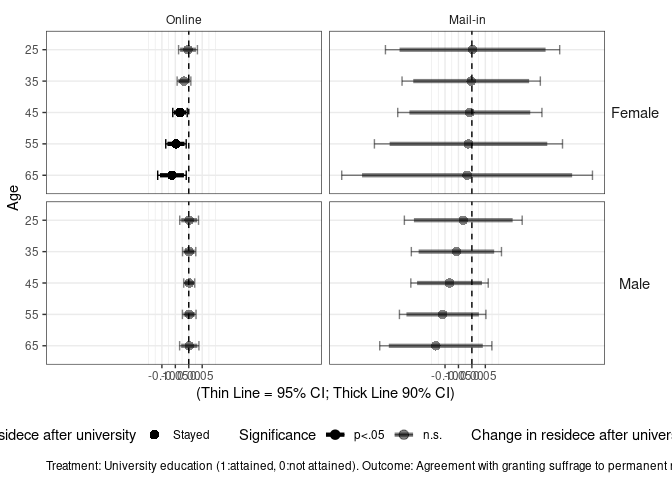
\includegraphics{analysis_1_original_mail_v5_files/figure-latex/unnamed-chunk-40-1.pdf}

\begin{Shaded}
\begin{Highlighting}[]
\KeywordTok{ggsave}\NormalTok{(}\KeywordTok{paste0}\NormalTok{(projdir,}\StringTok{"/out/mailineffectplot.png"}\NormalTok{),p,}\DataTypeTok{width=}\DecValTok{8}\NormalTok{,}\DataTypeTok{height=}\DecValTok{5}\NormalTok{)}
\end{Highlighting}
\end{Shaded}

\begin{verbatim}
## Warning: position_dodge requires non-overlapping x intervals

## Warning: position_dodge requires non-overlapping x intervals

## Warning: position_dodge requires non-overlapping x intervals

## Warning: position_dodge requires non-overlapping x intervals
\end{verbatim}

\begin{Shaded}
\begin{Highlighting}[]
\CommentTok{## Multinomial Logit ##}

\NormalTok{extout <-}\StringTok{ }\ControlFlowTok{function}\NormalTok{(gender,ageset,}\DataTypeTok{sub=}\DecValTok{1}\NormalTok{) \{}
  
  \ControlFlowTok{if}\NormalTok{ (gender}\OperatorTok{==}\StringTok{"Male"}\NormalTok{) sifcct}\OperatorTok{$}\NormalTok{gender <-}\StringTok{ }\NormalTok{sifcct}\OperatorTok{$}\NormalTok{female}
  \ControlFlowTok{if}\NormalTok{ (gender}\OperatorTok{==}\StringTok{"Female"}\NormalTok{) sifcct}\OperatorTok{$}\NormalTok{gender <-}\StringTok{ }\NormalTok{sifcct}\OperatorTok{$}\NormalTok{male}
\NormalTok{  sifcct}\OperatorTok{$}\NormalTok{ageset <-}\StringTok{ }\NormalTok{(sifcct}\OperatorTok{$}\NormalTok{age }\OperatorTok{-}\StringTok{ }\NormalTok{ageset)}\OperatorTok{/}\DecValTok{10}
  
  \ControlFlowTok{if}\NormalTok{ (sub}\OperatorTok{==}\DecValTok{1}\NormalTok{) \{}
    \CommentTok{# modset <- multinom(foreignsuff3x ~ edu2 * gender * ageset + lvpr + zip_did + sqrt(c10_sreg_fper) + }
    \CommentTok{#                      I(c10_sreg_edu_ugsP/10) + didper + sqrt(c10_mun_fper) + I(c10_mun_edu_ugsP/10) + }
    \CommentTok{#                      as.factor(wave), data=sifcct[which(sifcct$age - sifcct$lvlen<=15),],}
    \CommentTok{#                    Hess = TRUE)}
\NormalTok{    sifcct.mlogit.tmp <-}\StringTok{ }\KeywordTok{dfidx}\NormalTok{(sifcct[}\KeywordTok{which}\NormalTok{(sifcct}\OperatorTok{$}\NormalTok{age }\OperatorTok{-}\StringTok{ }\NormalTok{sifcct}\OperatorTok{$}\NormalTok{lvlen}\OperatorTok{<=}\DecValTok{15}\NormalTok{),],}
                           \DataTypeTok{shape =} \StringTok{"wide"}\NormalTok{, }\DataTypeTok{choice =} \StringTok{"foreignsuff3x"}\NormalTok{)}
    \CommentTok{# levels(sifcct.mlogit.tmp$idx$id2) <- c("Disagree","Neither","Agree")}
\NormalTok{    modset <-}\StringTok{ }\KeywordTok{mlogit}\NormalTok{(foreignsuff3x }\OperatorTok{~}\StringTok{ }\DecValTok{0} \OperatorTok{|}\StringTok{ }\NormalTok{edu2 }\OperatorTok{*}\StringTok{ }\NormalTok{gender }\OperatorTok{*}\StringTok{ }\NormalTok{ageset }\OperatorTok{+}\StringTok{ }\NormalTok{lvpr }\OperatorTok{+}\StringTok{ }\NormalTok{zip_did }\OperatorTok{+}\StringTok{ }\KeywordTok{sqrt}\NormalTok{(c10_sreg_fper) }\OperatorTok{+}\StringTok{ }
\StringTok{                         }\KeywordTok{I}\NormalTok{(c10_sreg_edu_ugsP}\OperatorTok{/}\DecValTok{10}\NormalTok{) }\OperatorTok{+}\StringTok{ }\NormalTok{didper }\OperatorTok{+}\StringTok{ }\KeywordTok{sqrt}\NormalTok{(c10_mun_fper) }\OperatorTok{+}\StringTok{ }\KeywordTok{I}\NormalTok{(c10_mun_edu_ugsP}\OperatorTok{/}\DecValTok{10}\NormalTok{) }\OperatorTok{+}\StringTok{ }
\StringTok{                         }\KeywordTok{as.factor}\NormalTok{(wave), }\DataTypeTok{data=}\NormalTok{sifcct.mlogit.tmp, }\DataTypeTok{reflevel=}\StringTok{"Disagree"}\NormalTok{)}
\NormalTok{    subname =}\StringTok{ "Stayed"}
\NormalTok{  \} }\ControlFlowTok{else}\NormalTok{ \{}
    \CommentTok{# modset <- multinom(foreignsuff3x ~ edu2 * gender * ageset + lvpr + as.factor(wave), }
    \CommentTok{#                    data=sifcct[which(sifcct$age - sifcct$lvlen>=23),],}
    \CommentTok{#                    Hess = TRUE)}
\NormalTok{    sifcct.mlogit.tmp <-}\StringTok{ }\KeywordTok{dfidx}\NormalTok{(sifcct[}\KeywordTok{which}\NormalTok{(sifcct}\OperatorTok{$}\NormalTok{age }\OperatorTok{-}\StringTok{ }\NormalTok{sifcct}\OperatorTok{$}\NormalTok{lvlen}\OperatorTok{>=}\DecValTok{23}\NormalTok{),],}
                           \DataTypeTok{shape =} \StringTok{"wide"}\NormalTok{, }\DataTypeTok{choice =} \StringTok{"foreignsuff3x"}\NormalTok{)}
    \CommentTok{# levels(sifcct.mlogit.tmp$idx$id2) <- c("Disagree","Neither","Agree")}
\NormalTok{    modset <-}\StringTok{ }\KeywordTok{mlogit}\NormalTok{(foreignsuff3x }\OperatorTok{~}\StringTok{ }\DecValTok{0} \OperatorTok{|}\StringTok{ }\NormalTok{edu2 }\OperatorTok{*}\StringTok{ }\NormalTok{gender }\OperatorTok{*}\StringTok{ }\NormalTok{ageset }\OperatorTok{+}\StringTok{ }\NormalTok{lvpr }\OperatorTok{+}\StringTok{ }\KeywordTok{as.factor}\NormalTok{(wave), }
                       \DataTypeTok{data=}\NormalTok{sifcct.mlogit.tmp, }\DataTypeTok{reflevel=}\StringTok{"Disagree"}\NormalTok{)}
\NormalTok{    subname =}\StringTok{ "Moved"}
\NormalTok{  \}}

  \CommentTok{# modres <- extract(modset)}
  
  \CommentTok{# res <- c(gender,ageset,modres@coef[grep("^Agree: edu2$",modres@coef.names)],}
  \CommentTok{#          modres@coef[grep("^Agree: edu2$",modres@coef.names)] - qnorm(0.975)*modres@se[grep("^Agree: edu2$",modres@coef.names)],}
  \CommentTok{#          modres@coef[grep("^Agree: edu2$",modres@coef.names)] + qnorm(0.975)*modres@se[grep("^Agree: edu2$",modres@coef.names)],}
  \CommentTok{#          modres@coef[grep("^Agree: edu2$",modres@coef.names)] - qnorm(0.95)*modres@se[grep("^Agree: edu2$",modres@coef.names)],}
  \CommentTok{#          modres@coef[grep("^Agree: edu2$",modres@coef.names)] + qnorm(0.95)*modres@se[grep("^Agree: edu2$",modres@coef.names)],}
  \CommentTok{#          modres@se[grep("^Agree: edu2$",modres@coef.names)],}
  \CommentTok{#          modres@pvalues[grep("^Agree: edu2$",modres@coef.names)],}
  \CommentTok{#          subname)}
\NormalTok{  res <-}\StringTok{ }\KeywordTok{c}\NormalTok{(gender,ageset,}\KeywordTok{coef}\NormalTok{(modset)[}\DecValTok{3}\NormalTok{],}
           \KeywordTok{coefci}\NormalTok{(modset, }\DataTypeTok{vcov=}\NormalTok{sandwich, }\DataTypeTok{level =} \FloatTok{0.95}\NormalTok{)[}\DecValTok{3}\NormalTok{,],}
           \KeywordTok{coefci}\NormalTok{(modset, }\DataTypeTok{vcov=}\NormalTok{sandwich, }\DataTypeTok{level =} \FloatTok{0.90}\NormalTok{)[}\DecValTok{3}\NormalTok{,],}
           \KeywordTok{coeftest}\NormalTok{(modset, }\DataTypeTok{vcov=}\NormalTok{sandwich)[}\DecValTok{3}\NormalTok{,}\KeywordTok{c}\NormalTok{(}\DecValTok{2}\NormalTok{,}\DecValTok{4}\NormalTok{)],}
\NormalTok{           subname)}
  
  \KeywordTok{names}\NormalTok{(res) <-}\StringTok{ }\KeywordTok{c}\NormalTok{(}\StringTok{"gender"}\NormalTok{,}\StringTok{"age"}\NormalTok{,}\StringTok{"est"}\NormalTok{,}\StringTok{"lci95"}\NormalTok{,}\StringTok{"uci95"}\NormalTok{,}\StringTok{"lci90"}\NormalTok{,}\StringTok{"uci90"}\NormalTok{,}\StringTok{"se"}\NormalTok{,}\StringTok{"p"}\NormalTok{,}\StringTok{"lv"}\NormalTok{)}
  
  \KeywordTok{return}\NormalTok{(res)}
  
\NormalTok{\}}

\NormalTok{outdt0 <-}\StringTok{ }\KeywordTok{rbind}\NormalTok{(}\KeywordTok{extout}\NormalTok{(}\StringTok{"Female"}\NormalTok{,}\DecValTok{25}\NormalTok{,}\DecValTok{1}\NormalTok{),}
                 \KeywordTok{extout}\NormalTok{(}\StringTok{"Female"}\NormalTok{,}\DecValTok{35}\NormalTok{,}\DecValTok{1}\NormalTok{),}
                 \KeywordTok{extout}\NormalTok{(}\StringTok{"Female"}\NormalTok{,}\DecValTok{45}\NormalTok{,}\DecValTok{1}\NormalTok{),}
                 \KeywordTok{extout}\NormalTok{(}\StringTok{"Female"}\NormalTok{,}\DecValTok{55}\NormalTok{,}\DecValTok{1}\NormalTok{),}
                 \KeywordTok{extout}\NormalTok{(}\StringTok{"Female"}\NormalTok{,}\DecValTok{65}\NormalTok{,}\DecValTok{1}\NormalTok{),}
                 \KeywordTok{extout}\NormalTok{(}\StringTok{"Male"}\NormalTok{,}\DecValTok{25}\NormalTok{,}\DecValTok{1}\NormalTok{),}
                 \KeywordTok{extout}\NormalTok{(}\StringTok{"Male"}\NormalTok{,}\DecValTok{35}\NormalTok{,}\DecValTok{1}\NormalTok{),}
                 \KeywordTok{extout}\NormalTok{(}\StringTok{"Male"}\NormalTok{,}\DecValTok{45}\NormalTok{,}\DecValTok{1}\NormalTok{),}
                 \KeywordTok{extout}\NormalTok{(}\StringTok{"Male"}\NormalTok{,}\DecValTok{55}\NormalTok{,}\DecValTok{1}\NormalTok{),}
                 \KeywordTok{extout}\NormalTok{(}\StringTok{"Male"}\NormalTok{,}\DecValTok{65}\NormalTok{,}\DecValTok{1}\NormalTok{))}
\NormalTok{outdt0 <-}\StringTok{ }\KeywordTok{as.data.frame}\NormalTok{(outdt0)}
\ControlFlowTok{for}\NormalTok{(i }\ControlFlowTok{in} \DecValTok{2}\OperatorTok{:}\DecValTok{9}\NormalTok{) outdt0[,i] <-}\StringTok{ }\KeywordTok{as.numeric}\NormalTok{(outdt0[,i])}
\NormalTok{outdt0}\OperatorTok{$}\NormalTok{gender <-}\StringTok{ }\KeywordTok{factor}\NormalTok{(outdt0}\OperatorTok{$}\NormalTok{gender, }\DataTypeTok{levels=}\KeywordTok{unique}\NormalTok{(outdt0}\OperatorTok{$}\NormalTok{gender))}
\KeywordTok{summary}\NormalTok{(outdt0)}
\end{Highlighting}
\end{Shaded}

\begin{verbatim}
##     gender       age          est               lci95              uci95               lci90         
##  Female:5   Min.   :25   Min.   :-0.44832   Min.   :-0.84560   Min.   :-0.052650   Min.   :-0.78171  
##  Male  :5   1st Qu.:35   1st Qu.:-0.19705   1st Qu.:-0.39904   1st Qu.: 0.004953   1st Qu.:-0.36656  
##             Median :45   Median : 0.01565   Median :-0.24651   Median : 0.241227   Median :-0.20435  
##             Mean   :45   Mean   :-0.06611   Mean   :-0.30558   Mean   : 0.173355   Mean   :-0.26707  
##             3rd Qu.:55   3rd Qu.: 0.08526   3rd Qu.:-0.11455   3rd Qu.: 0.280028   3rd Qu.:-0.07653  
##             Max.   :65   Max.   : 0.15257   Max.   :-0.05757   Max.   : 0.422067   Max.   :-0.03340  
##      uci90                se                p                lv           
##  Min.   :-0.11494   Min.   :0.07668   Min.   :0.02017   Length:10         
##  1st Qu.:-0.02753   1st Qu.:0.09837   1st Qu.:0.07434   Class :character  
##  Median : 0.21494   Median :0.11539   Median :0.24534   Mode  :character  
##  Mean   : 0.13485   Mean   :0.12216   Mean   :0.33148                     
##  3rd Qu.: 0.23890   3rd Qu.:0.13957   3rd Qu.:0.43096                     
##  Max.   : 0.37873   Max.   :0.20266   Max.   :0.99087
\end{verbatim}

\begin{Shaded}
\begin{Highlighting}[]
\NormalTok{extout <-}\StringTok{ }\ControlFlowTok{function}\NormalTok{(gender,ageset,}\DataTypeTok{sub=}\DecValTok{1}\NormalTok{) \{}
  
  \ControlFlowTok{if}\NormalTok{ (gender}\OperatorTok{==}\StringTok{"Male"}\NormalTok{) mail}\OperatorTok{$}\NormalTok{gender <-}\StringTok{ }\NormalTok{mail}\OperatorTok{$}\NormalTok{female}
  \ControlFlowTok{if}\NormalTok{ (gender}\OperatorTok{==}\StringTok{"Female"}\NormalTok{) mail}\OperatorTok{$}\NormalTok{gender <-}\StringTok{ }\NormalTok{mail}\OperatorTok{$}\NormalTok{male}
\NormalTok{  mail}\OperatorTok{$}\NormalTok{ageset <-}\StringTok{ }\NormalTok{(mail}\OperatorTok{$}\NormalTok{age }\OperatorTok{-}\StringTok{ }\NormalTok{ageset)}\OperatorTok{/}\DecValTok{10}
  
  \ControlFlowTok{if}\NormalTok{ (sub}\OperatorTok{==}\DecValTok{1}\NormalTok{) \{}
    \CommentTok{# modset <- multinom(foreignsuff3x ~ edu2 * gender * ageset + lvpr + zip_did + sqrt(c10_sreg_fper) +}
    \CommentTok{#                      I(c10_sreg_edu_ugsP/10) + didper + sqrt(c10_mun_fper) + I(c10_mun_edu_ugsP/10),}
    \CommentTok{#                    data=mail[which(mail$age - mail$lvlen<=15),],}
    \CommentTok{#                    Hess = TRUE)}
\NormalTok{    mail.mlogit.tmp <-}\StringTok{ }\KeywordTok{dfidx}\NormalTok{(mail[}\KeywordTok{which}\NormalTok{(mail}\OperatorTok{$}\NormalTok{age }\OperatorTok{-}\StringTok{ }\NormalTok{mail}\OperatorTok{$}\NormalTok{lvlen}\OperatorTok{<=}\DecValTok{15}\NormalTok{),],}
                               \DataTypeTok{shape =} \StringTok{"wide"}\NormalTok{, }\DataTypeTok{choice =} \StringTok{"foreignsuff3x"}\NormalTok{)}
    \CommentTok{# levels(mail.mlogit.tmp$idx$id2) <- c("Disagree","Neither","Agree")}
\NormalTok{    modset <-}\StringTok{ }\KeywordTok{mlogit}\NormalTok{(foreignsuff3x }\OperatorTok{~}\StringTok{ }\DecValTok{0} \OperatorTok{|}\StringTok{ }\NormalTok{edu2 }\OperatorTok{*}\StringTok{ }\NormalTok{gender }\OperatorTok{*}\StringTok{ }\NormalTok{ageset }\OperatorTok{+}\StringTok{ }\NormalTok{lvpr }\OperatorTok{+}\StringTok{ }\NormalTok{zip_did }\OperatorTok{+}\StringTok{ }\KeywordTok{sqrt}\NormalTok{(c10_sreg_fper) }\OperatorTok{+}\StringTok{ }
\StringTok{                       }\KeywordTok{I}\NormalTok{(c10_sreg_edu_ugsP}\OperatorTok{/}\DecValTok{10}\NormalTok{) }\OperatorTok{+}\StringTok{ }\NormalTok{didper }\OperatorTok{+}\StringTok{ }\KeywordTok{sqrt}\NormalTok{(c10_mun_fper) }\OperatorTok{+}\StringTok{ }\KeywordTok{I}\NormalTok{(c10_mun_edu_ugsP}\OperatorTok{/}\DecValTok{10}\NormalTok{), }
                     \DataTypeTok{data=}\NormalTok{mail.mlogit.tmp, }\DataTypeTok{reflevel=}\StringTok{"Disagree"}\NormalTok{)}
\NormalTok{    subname =}\StringTok{ "Stayed"}
\NormalTok{  \} }\ControlFlowTok{else}\NormalTok{ \{}
    \CommentTok{# modset <- multinom(foreignsuff3x ~ edu2 * gender * ageset + lvpr, }
    \CommentTok{#                    data=mail[which(mail$age - mail$lvlen>=23),],}
    \CommentTok{#                    Hess = TRUE)}
\NormalTok{    mail.mlogit.tmp <-}\StringTok{ }\KeywordTok{dfidx}\NormalTok{(mail[}\KeywordTok{which}\NormalTok{(mail}\OperatorTok{$}\NormalTok{age }\OperatorTok{-}\StringTok{ }\NormalTok{mail}\OperatorTok{$}\NormalTok{lvlen}\OperatorTok{>=}\DecValTok{23}\NormalTok{),],}
                               \DataTypeTok{shape =} \StringTok{"wide"}\NormalTok{, }\DataTypeTok{choice =} \StringTok{"foreignsuff3x"}\NormalTok{)}
    \CommentTok{# levels(mail.mlogit.tmp$idx$id2) <- c("Disagree","Neither","Agree")}
\NormalTok{    modset <-}\StringTok{ }\KeywordTok{mlogit}\NormalTok{(foreignsuff3x }\OperatorTok{~}\StringTok{ }\DecValTok{0} \OperatorTok{|}\StringTok{ }\NormalTok{edu2 }\OperatorTok{*}\StringTok{ }\NormalTok{gender }\OperatorTok{*}\StringTok{ }\NormalTok{ageset }\OperatorTok{+}\StringTok{ }\NormalTok{lvpr, }
                     \DataTypeTok{data=}\NormalTok{mail.mlogit.tmp, }\DataTypeTok{reflevel=}\StringTok{"Disagree"}\NormalTok{)}
\NormalTok{    subname =}\StringTok{ "Moved"}
\NormalTok{  \}}
  
  \CommentTok{# modres <- extract(modset)}
  
  \CommentTok{# res <- c(gender,ageset,modres@coef[grep("^Agree: edu2$",modres@coef.names)],}
  \CommentTok{#          modres@coef[grep("^Agree: edu2$",modres@coef.names)] - qnorm(0.975)*modres@se[grep("^Agree: edu2$",modres@coef.names)],}
  \CommentTok{#          modres@coef[grep("^Agree: edu2$",modres@coef.names)] + qnorm(0.975)*modres@se[grep("^Agree: edu2$",modres@coef.names)],}
  \CommentTok{#          modres@coef[grep("^Agree: edu2$",modres@coef.names)] - qnorm(0.95)*modres@se[grep("^Agree: edu2$",modres@coef.names)],}
  \CommentTok{#          modres@coef[grep("^Agree: edu2$",modres@coef.names)] + qnorm(0.95)*modres@se[grep("^Agree: edu2$",modres@coef.names)],}
  \CommentTok{#          modres@se[grep("^Agree: edu2$",modres@coef.names)],}
  \CommentTok{#          modres@pvalues[grep("^Agree: edu2$",modres@coef.names)],}
  \CommentTok{#          subname)}
\NormalTok{  res <-}\StringTok{ }\KeywordTok{c}\NormalTok{(gender,ageset,}\KeywordTok{coef}\NormalTok{(modset)[}\DecValTok{3}\NormalTok{],}
           \KeywordTok{coefci}\NormalTok{(modset, }\DataTypeTok{vcov=}\NormalTok{sandwich, }\DataTypeTok{level =} \FloatTok{0.95}\NormalTok{)[}\DecValTok{3}\NormalTok{,],}
           \KeywordTok{coefci}\NormalTok{(modset, }\DataTypeTok{vcov=}\NormalTok{sandwich, }\DataTypeTok{level =} \FloatTok{0.90}\NormalTok{)[}\DecValTok{3}\NormalTok{,],}
           \KeywordTok{coeftest}\NormalTok{(modset, }\DataTypeTok{vcov=}\NormalTok{sandwich)[}\DecValTok{3}\NormalTok{,}\KeywordTok{c}\NormalTok{(}\DecValTok{2}\NormalTok{,}\DecValTok{4}\NormalTok{)],}
\NormalTok{           subname)}
  
  \KeywordTok{names}\NormalTok{(res) <-}\StringTok{ }\KeywordTok{c}\NormalTok{(}\StringTok{"gender"}\NormalTok{,}\StringTok{"age"}\NormalTok{,}\StringTok{"est"}\NormalTok{,}\StringTok{"lci95"}\NormalTok{,}\StringTok{"uci95"}\NormalTok{,}\StringTok{"lci90"}\NormalTok{,}\StringTok{"uci90"}\NormalTok{,}\StringTok{"se"}\NormalTok{,}\StringTok{"p"}\NormalTok{,}\StringTok{"lv"}\NormalTok{)}
  
  \KeywordTok{return}\NormalTok{(res)}
  
\NormalTok{\}}

\NormalTok{outdtm <-}\StringTok{ }\KeywordTok{rbind}\NormalTok{(}\KeywordTok{extout}\NormalTok{(}\StringTok{"Female"}\NormalTok{,}\DecValTok{25}\NormalTok{,}\DecValTok{1}\NormalTok{),}
                 \KeywordTok{extout}\NormalTok{(}\StringTok{"Female"}\NormalTok{,}\DecValTok{35}\NormalTok{,}\DecValTok{1}\NormalTok{),}
                 \KeywordTok{extout}\NormalTok{(}\StringTok{"Female"}\NormalTok{,}\DecValTok{45}\NormalTok{,}\DecValTok{1}\NormalTok{),}
                 \KeywordTok{extout}\NormalTok{(}\StringTok{"Female"}\NormalTok{,}\DecValTok{55}\NormalTok{,}\DecValTok{1}\NormalTok{),}
                 \KeywordTok{extout}\NormalTok{(}\StringTok{"Female"}\NormalTok{,}\DecValTok{65}\NormalTok{,}\DecValTok{1}\NormalTok{),}
                 \KeywordTok{extout}\NormalTok{(}\StringTok{"Male"}\NormalTok{,}\DecValTok{25}\NormalTok{,}\DecValTok{1}\NormalTok{),}
                 \KeywordTok{extout}\NormalTok{(}\StringTok{"Male"}\NormalTok{,}\DecValTok{35}\NormalTok{,}\DecValTok{1}\NormalTok{),}
                 \KeywordTok{extout}\NormalTok{(}\StringTok{"Male"}\NormalTok{,}\DecValTok{45}\NormalTok{,}\DecValTok{1}\NormalTok{),}
                 \KeywordTok{extout}\NormalTok{(}\StringTok{"Male"}\NormalTok{,}\DecValTok{55}\NormalTok{,}\DecValTok{1}\NormalTok{),}
                 \KeywordTok{extout}\NormalTok{(}\StringTok{"Male"}\NormalTok{,}\DecValTok{65}\NormalTok{,}\DecValTok{1}\NormalTok{))}
\NormalTok{outdtm <-}\StringTok{ }\KeywordTok{as.data.frame}\NormalTok{(outdtm)}
\ControlFlowTok{for}\NormalTok{(i }\ControlFlowTok{in} \DecValTok{2}\OperatorTok{:}\DecValTok{9}\NormalTok{) outdtm[,i] <-}\StringTok{ }\KeywordTok{as.numeric}\NormalTok{(outdtm[,i])}
\NormalTok{outdtm}\OperatorTok{$}\NormalTok{gender <-}\StringTok{ }\KeywordTok{factor}\NormalTok{(outdtm}\OperatorTok{$}\NormalTok{gender, }\DataTypeTok{levels=}\KeywordTok{unique}\NormalTok{(outdtm}\OperatorTok{$}\NormalTok{gender))}
\KeywordTok{summary}\NormalTok{(outdtm)}
\end{Highlighting}
\end{Shaded}

\begin{verbatim}
##     gender       age          est              lci95            uci95            lci90            uci90       
##  Female:5   Min.   :25   Min.   :-0.5684   Min.   :-2.987   Min.   :0.6797   Min.   :-2.595   Min.   :0.5222  
##  Male  :5   1st Qu.:35   1st Qu.:-0.3373   1st Qu.:-1.762   1st Qu.:0.9037   1st Qu.:-1.469   1st Qu.:0.7071  
##             Median :45   Median :-0.2075   Median :-1.590   Median :1.3569   Median :-1.367   Median :1.1130  
##             Mean   :45   Mean   :-0.2044   Mean   :-1.719   Mean   :1.3103   Mean   :-1.473   Mean   :1.0647  
##             3rd Qu.:55   3rd Qu.:-0.1338   3rd Qu.:-1.357   3rd Qu.:1.5994   3rd Qu.:-1.163   3rd Qu.:1.3281  
##             Max.   :65   Max.   : 0.2235   Max.   :-1.152   Max.   :2.2209   Max.   :-1.004   Max.   :1.8970  
##        se               p               lv           
##  Min.   :0.4640   Min.   :0.5521   Length:10         
##  1st Qu.:0.5785   1st Qu.:0.6192   Class :character  
##  Median :0.7616   Median :0.7236   Mode  :character  
##  Mean   :0.7673   Mean   :0.7329                     
##  3rd Qu.:0.9151   3rd Qu.:0.8266                     
##  Max.   :1.2253   Max.   :0.9750
\end{verbatim}

\begin{Shaded}
\begin{Highlighting}[]
\NormalTok{outdt0}\OperatorTok{$}\NormalTok{data <-}\StringTok{ "Online"}
\NormalTok{outdtm}\OperatorTok{$}\NormalTok{data <-}\StringTok{ "Mail-in"}

\NormalTok{visdt <-}\StringTok{ }\KeywordTok{rbind}\NormalTok{(outdt0,outdtm)}
\NormalTok{visdt}\OperatorTok{$}\NormalTok{data <-}\StringTok{ }\KeywordTok{factor}\NormalTok{(visdt}\OperatorTok{$}\NormalTok{data, }\DataTypeTok{levels=}\KeywordTok{c}\NormalTok{(}\StringTok{"Online"}\NormalTok{,}\StringTok{"Mail-in"}\NormalTok{))}

\NormalTok{visdt}\OperatorTok{$}\NormalTok{pstar <-}\StringTok{ }\KeywordTok{factor}\NormalTok{(}\KeywordTok{ifelse}\NormalTok{(visdt}\OperatorTok{$}\NormalTok{p}\OperatorTok{>=}\NormalTok{.}\DecValTok{1}\NormalTok{,}\StringTok{"n.s."}\NormalTok{,}\KeywordTok{ifelse}\NormalTok{(visdt}\OperatorTok{$}\NormalTok{p}\OperatorTok{>=}\NormalTok{.}\DecValTok{05}\NormalTok{,}\StringTok{"p<.1"}\NormalTok{,}\StringTok{"p<.05"}\NormalTok{)),}
                       \DataTypeTok{levels =} \KeywordTok{c}\NormalTok{(}\StringTok{"p<.05"}\NormalTok{,}\StringTok{"p<.1"}\NormalTok{,}\StringTok{"n.s."}\NormalTok{))}

\KeywordTok{saveRDS}\NormalTok{(}\KeywordTok{subset}\NormalTok{(visdt, data}\OperatorTok{==}\StringTok{"Mail-in"}\NormalTok{), }\KeywordTok{paste0}\NormalTok{(projdir, }\StringTok{"/out/visdt_mail_multinom.rds"}\NormalTok{))}

\KeywordTok{require}\NormalTok{(ggplot2)}
\NormalTok{p <-}\StringTok{ }\KeywordTok{ggplot}\NormalTok{(visdt, }\KeywordTok{aes}\NormalTok{(}\DataTypeTok{x=}\KeywordTok{factor}\NormalTok{(age, }\DataTypeTok{levels=}\KeywordTok{rev}\NormalTok{(}\KeywordTok{names}\NormalTok{(}\KeywordTok{table}\NormalTok{(age)))), }\DataTypeTok{y=}\NormalTok{est)) }\OperatorTok{+}
\StringTok{  }\KeywordTok{geom_hline}\NormalTok{(}\KeywordTok{aes}\NormalTok{(}\DataTypeTok{yintercept=}\DecValTok{0}\NormalTok{), }\DataTypeTok{linetype=}\DecValTok{2}\NormalTok{) }\OperatorTok{+}
\StringTok{  }\KeywordTok{geom_errorbar}\NormalTok{(}\KeywordTok{aes}\NormalTok{(}\DataTypeTok{ymin=}\NormalTok{lci95,}\DataTypeTok{ymax=}\NormalTok{uci95,}\DataTypeTok{colour=}\StringTok{"1"}\NormalTok{,}\DataTypeTok{alpha=}\NormalTok{pstar), }
                \DataTypeTok{position=}\KeywordTok{position_dodge}\NormalTok{(}\DataTypeTok{width=}\OperatorTok{-}\FloatTok{0.7}\NormalTok{), }\DataTypeTok{size=}\FloatTok{0.5}\NormalTok{, }\DataTypeTok{width=}\FloatTok{0.3}\NormalTok{) }\OperatorTok{+}
\StringTok{  }\KeywordTok{geom_errorbar}\NormalTok{(}\KeywordTok{aes}\NormalTok{(}\DataTypeTok{ymin=}\NormalTok{lci90,}\DataTypeTok{ymax=}\NormalTok{uci90,}\DataTypeTok{colour=}\StringTok{"1"}\NormalTok{,}\DataTypeTok{alpha=}\NormalTok{pstar),}
                \DataTypeTok{position=}\KeywordTok{position_dodge}\NormalTok{(}\DataTypeTok{width=}\OperatorTok{-}\FloatTok{0.7}\NormalTok{), }\DataTypeTok{size=}\FloatTok{1.5}\NormalTok{, }\DataTypeTok{width=}\FloatTok{0.0}\NormalTok{) }\OperatorTok{+}
\StringTok{  }\KeywordTok{geom_point}\NormalTok{(}\KeywordTok{aes}\NormalTok{(}\DataTypeTok{shape=}\NormalTok{lv, }\DataTypeTok{colour=}\StringTok{"1"}\NormalTok{,}\DataTypeTok{alpha=}\NormalTok{pstar),}
             \DataTypeTok{position=}\KeywordTok{position_dodge}\NormalTok{(}\DataTypeTok{width=}\OperatorTok{-}\FloatTok{0.7}\NormalTok{), }\DataTypeTok{size=}\DecValTok{3}\NormalTok{) }\OperatorTok{+}
\StringTok{  }\KeywordTok{facet_grid}\NormalTok{(gender }\OperatorTok{~}\StringTok{ }\NormalTok{data) }\OperatorTok{+}
\StringTok{  }\CommentTok{#scale_y_continuous(breaks = c(-0.1,-0.05,0.00,0.05)) + }
\StringTok{  }\KeywordTok{scale_shape_discrete}\NormalTok{(}\DataTypeTok{name=}\StringTok{"Change in residece after university"}\NormalTok{) }\OperatorTok{+}
\StringTok{  }\KeywordTok{scale_color_manual}\NormalTok{(}\DataTypeTok{name=}\StringTok{"Change in residece after university"}\NormalTok{,}\DataTypeTok{values=}\KeywordTok{rep}\NormalTok{(}\StringTok{"black"}\NormalTok{, }\DecValTok{1}\NormalTok{)) }\OperatorTok{+}
\StringTok{  }\KeywordTok{scale_alpha_manual}\NormalTok{(}\DataTypeTok{name=}\StringTok{"Significance"}\NormalTok{,}\DataTypeTok{values=}\KeywordTok{c}\NormalTok{(}\DecValTok{1}\NormalTok{,}\FloatTok{0.5}\NormalTok{,}\FloatTok{0.2}\NormalTok{)) }\OperatorTok{+}
\StringTok{  }\KeywordTok{ylab}\NormalTok{(}\StringTok{"(Thin Line = 95% CI; Thick Line 90% CI)"}\NormalTok{) }\OperatorTok{+}
\StringTok{  }\KeywordTok{xlab}\NormalTok{(}\StringTok{"Age"}\NormalTok{) }\OperatorTok{+}
\StringTok{  }\KeywordTok{labs}\NormalTok{(}\DataTypeTok{caption=}\StringTok{"Treatment: University education (1:attained, 0:not attained). Outcome: Agreement with granting suffrage to permanent residents (rescaled to 0-1)."}\NormalTok{) }\OperatorTok{+}
\StringTok{  }\KeywordTok{coord_flip}\NormalTok{() }\OperatorTok{+}\StringTok{ }\KeywordTok{theme_bw}\NormalTok{() }\OperatorTok{+}
\StringTok{  }\KeywordTok{theme}\NormalTok{(}\DataTypeTok{legend.position =} \StringTok{"bottom"}\NormalTok{,}
        \DataTypeTok{strip.text.x =} \KeywordTok{element_text}\NormalTok{(}\DataTypeTok{size=}\DecValTok{9}\NormalTok{),}
        \DataTypeTok{strip.text.y =} \KeywordTok{element_text}\NormalTok{(}\DataTypeTok{angle=}\DecValTok{0}\NormalTok{,}\DataTypeTok{size=}\DecValTok{11}\NormalTok{),}
        \DataTypeTok{strip.background =} \KeywordTok{element_rect}\NormalTok{(}\DataTypeTok{fill=}\OtherTok{NA}\NormalTok{,}\DataTypeTok{color=}\OtherTok{NA}\NormalTok{),}
        \DataTypeTok{plot.caption =} \KeywordTok{element_text}\NormalTok{(}\DataTypeTok{hjust=}\DecValTok{0}\NormalTok{),}
        \DataTypeTok{plot.subtitle =} \KeywordTok{element_text}\NormalTok{(}\DataTypeTok{hjust=}\FloatTok{0.5}\NormalTok{))}
\NormalTok{p}
\end{Highlighting}
\end{Shaded}

\begin{verbatim}
## Warning: position_dodge requires non-overlapping x intervals

## Warning: position_dodge requires non-overlapping x intervals

## Warning: position_dodge requires non-overlapping x intervals

## Warning: position_dodge requires non-overlapping x intervals
\end{verbatim}

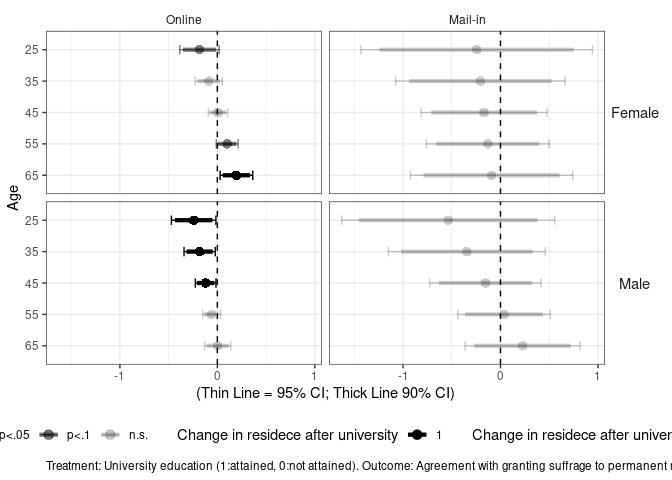
\includegraphics{analysis_1_original_mail_v5_files/figure-latex/unnamed-chunk-40-2.pdf}

\begin{Shaded}
\begin{Highlighting}[]
\KeywordTok{ggsave}\NormalTok{(}\KeywordTok{paste0}\NormalTok{(projdir,}\StringTok{"/out/mailineffectplot_multinom.png"}\NormalTok{),p,}\DataTypeTok{width=}\DecValTok{8}\NormalTok{,}\DataTypeTok{height=}\DecValTok{5}\NormalTok{)}
\end{Highlighting}
\end{Shaded}

\begin{verbatim}
## Warning: position_dodge requires non-overlapping x intervals

## Warning: position_dodge requires non-overlapping x intervals

## Warning: position_dodge requires non-overlapping x intervals

## Warning: position_dodge requires non-overlapping x intervals
\end{verbatim}

\hypertarget{save-image}{%
\section{Save Image}\label{save-image}}

\begin{Shaded}
\begin{Highlighting}[]
\KeywordTok{save.image}\NormalTok{(}\DataTypeTok{file=}\KeywordTok{paste0}\NormalTok{(projdir,}\StringTok{"/out/heavy/analysis_1_original_mail_v5.RData"}\NormalTok{))}
\end{Highlighting}
\end{Shaded}

\end{document}
